\PassOptionsToPackage{table}{xcolor}
\documentclass{article}
\usepackage{preprint}
\usepackage{newtxtext,newtxmath}
\usepackage{microtype}
\usepackage{graphicx}
\usepackage{booktabs}
\usepackage{multirow}   % header labels that span both rows of a two-row header, so they centre vertically
\usepackage{float}
\usepackage{placeins}
\usepackage{longtable}
\usepackage{enumitem}
\usepackage{amsmath}
\let\Bbbk\relax
\usepackage{amssymb}
\usepackage{xcolor}
\usepackage{url}
\usepackage{hyperref}
\hypersetup{hidelinks}
\newcommand{\R}{\mathbb{R}}
\newcommand{\E}{\mathbb{E}}
\newcommand{\hvec}{\mathbf{h}}
\newcommand{\wvec}{\mathbf{w}}
\newcommand{\vvec}{\mathbf{v}}
\newcommand{\DeltaEff}{\Delta_{\mathrm{Eff}}}
\DeclareMathOperator*{\argmaxop}{arg\,max}
\providecommand{\fitwidth}[1]{\resizebox{\ifdim\width>\linewidth\linewidth\else\width\fi}{!}{#1}}

% terracotta = positive / high, blue = negative / low, sage = magnitude of Read and Ans; darker = larger magnitude
\definecolor{cfSage1}{HTML}{ECF3EF}
\definecolor{cfSage2}{HTML}{D5E5DB}
\definecolor{cfSage3}{HTML}{B9D4C3}
\definecolor{cfSage4}{HTML}{9EC3AC}
\definecolor{cfSlate1}{HTML}{EAF0F6}
\definecolor{cfSlate2}{HTML}{D0DDEA}
\definecolor{cfSlate3}{HTML}{B1C7DD}
\definecolor{cfSlate4}{HTML}{94B2D0}
\definecolor{cfTerra1}{HTML}{F7ECEA}
\definecolor{cfTerra2}{HTML}{EED5D1}
\definecolor{cfTerra3}{HTML}{E2B8B2}
\definecolor{cfTerra4}{HTML}{D79E95}
\definecolor{cfOat1}{HTML}{F4EFE6}
\definecolor{cfOat2}{HTML}{E8DDC8}
\definecolor{cfGrey}{HTML}{E4E1DC}

% Generated by scripts/build_numbers.py from runs/manifest.csv; do not edit.
% Rule: a block enters the write-matrix counts iff run.json completed_modules contains CORE and CALIBRATION;
% readability counts run over probe-graded cells (CALIBRATION completed). See scripts/cf_inclusion.py.
% 75 blocks, 75 included, 450 write-matrix cells, 450 probe-graded cells.
\providecommand{\cfCheckpoints}{}\renewcommand{\cfCheckpoints}{25}
\providecommand{\cfBlocks}{}\renewcommand{\cfBlocks}{75}
\providecommand{\cfWriteBlocks}{}\renewcommand{\cfWriteBlocks}{75}
\providecommand{\cfProbeBlocks}{}\renewcommand{\cfProbeBlocks}{75}
\providecommand{\cfCells}{}\renewcommand{\cfCells}{450}
\providecommand{\cfProbeCells}{}\renewcommand{\cfProbeCells}{450}
\providecommand{\cfChestBlocks}{}\renewcommand{\cfChestBlocks}{50}
\providecommand{\cfChestProbeBlocks}{}\renewcommand{\cfChestProbeBlocks}{50}
\providecommand{\cfNihBlocks}{}\renewcommand{\cfNihBlocks}{25}
\providecommand{\cfChexBlocks}{}\renewcommand{\cfChexBlocks}{25}
\providecommand{\cfCocoBlocks}{}\renewcommand{\cfCocoBlocks}{25}
\providecommand{\cfCheckpointsComplete}{}\renewcommand{\cfCheckpointsComplete}{25}
\providecommand{\cfCheckpointsCompleteWord}{}\renewcommand{\cfCheckpointsCompleteWord}{Twenty-five}
\providecommand{\cfChestReadable}{}\renewcommand{\cfChestReadable}{256}
\providecommand{\cfChestReadableN}{}\renewcommand{\cfChestReadableN}{300}
\providecommand{\cfChestReadablePct}{}\renewcommand{\cfChestReadablePct}{85}
\providecommand{\cfChestAnswerable}{}\renewcommand{\cfChestAnswerable}{257}
\providecommand{\cfChestAnswerableN}{}\renewcommand{\cfChestAnswerableN}{300}
\providecommand{\cfChestCellsN}{}\renewcommand{\cfChestCellsN}{300}
\providecommand{\cfChestAnswerablePct}{}\renewcommand{\cfChestAnswerablePct}{86}
\providecommand{\cfChestOwned}{}\renewcommand{\cfChestOwned}{44}
\providecommand{\cfChestOwnedPct}{}\renewcommand{\cfChestOwnedPct}{15}
\providecommand{\cfChestCompetitor}{}\renewcommand{\cfChestCompetitor}{219}
\providecommand{\cfChestCompetitorPct}{}\renewcommand{\cfChestCompetitorPct}{73}
\providecommand{\cfChestRefMet}{}\renewcommand{\cfChestRefMet}{56}
\providecommand{\cfChestRefBelow}{}\renewcommand{\cfChestRefBelow}{244}
\providecommand{\cfChestRefNotOwned}{}\renewcommand{\cfChestRefNotOwned}{12}
\providecommand{\cfChestRefStrong}{}\renewcommand{\cfChestRefStrong}{12}
\providecommand{\cfChestRefUnres}{}\renewcommand{\cfChestRefUnres}{0}
\providecommand{\cfChestBelowAdv}{}\renewcommand{\cfChestBelowAdv}{37}
\providecommand{\cfChestBelowStrong}{}\renewcommand{\cfChestBelowStrong}{207}
\providecommand{\cfChestBelowUnres}{}\renewcommand{\cfChestBelowUnres}{0}
\providecommand{\cfReadAnsRefMet}{}\renewcommand{\cfReadAnsRefMet}{50}
\providecommand{\cfReadAnsRefBelow}{}\renewcommand{\cfReadAnsRefBelow}{188}
\providecommand{\cfReadAnsCompetitor}{}\renewcommand{\cfReadAnsCompetitor}{170}
\providecommand{\cfReadAnsRefStrong}{}\renewcommand{\cfReadAnsRefStrong}{10}
\providecommand{\cfReadAnsRefUnres}{}\renewcommand{\cfReadAnsRefUnres}{0}
\providecommand{\cfReadAnsBelowAdv}{}\renewcommand{\cfReadAnsBelowAdv}{28}
\providecommand{\cfReadAnsBelowStrong}{}\renewcommand{\cfReadAnsBelowStrong}{160}
\providecommand{\cfReadAnsBelowUnres}{}\renewcommand{\cfReadAnsBelowUnres}{0}
\providecommand{\cfCocoRefStrong}{}\renewcommand{\cfCocoRefStrong}{0}
\providecommand{\cfCocoRefUnres}{}\renewcommand{\cfCocoRefUnres}{0}
\providecommand{\cfCocoBelowAdv}{}\renewcommand{\cfCocoBelowAdv}{12}
\providecommand{\cfCocoBelowStrong}{}\renewcommand{\cfCocoBelowStrong}{21}
\providecommand{\cfCocoBelowUnres}{}\renewcommand{\cfCocoBelowUnres}{0}
\providecommand{\cfChestBelowStrongPct}{}\renewcommand{\cfChestBelowStrongPct}{95}
\providecommand{\cfReadAns}{}\renewcommand{\cfReadAns}{238}
\providecommand{\cfReadAnsOwned}{}\renewcommand{\cfReadAnsOwned}{40}
\providecommand{\cfReadAnsOwnedPct}{}\renewcommand{\cfReadAnsOwnedPct}{17}
\providecommand{\cfRestN}{}\renewcommand{\cfRestN}{62}
\providecommand{\cfRestOwned}{}\renewcommand{\cfRestOwned}{4}
\providecommand{\cfRestOwnedPct}{}\renewcommand{\cfRestOwnedPct}{6}
\providecommand{\cfChestFloored}{}\renewcommand{\cfChestFloored}{18}
\providecommand{\cfChestFlooredPct}{}\renewcommand{\cfChestFlooredPct}{6}
\providecommand{\cfEffusionOwnedBlocks}{}\renewcommand{\cfEffusionOwnedBlocks}{8}
\providecommand{\cfEffusionOwnedSmall}{}\renewcommand{\cfEffusionOwnedSmall}{7}
\providecommand{\cfSelEffusion}{}\renewcommand{\cfSelEffusion}{0.18}
\providecommand{\cfSelCardiomegaly}{}\renewcommand{\cfSelCardiomegaly}{0.19}
\providecommand{\cfSelChestMed}{}\renewcommand{\cfSelChestMed}{0.14}
\providecommand{\cfSelChestQOne}{}\renewcommand{\cfSelChestQOne}{0.08}
\providecommand{\cfSelChestQThree}{}\renewcommand{\cfSelChestQThree}{0.22}
\providecommand{\cfSelChestN}{}\renewcommand{\cfSelChestN}{300}
\providecommand{\cfNihReadable}{}\renewcommand{\cfNihReadable}{135}
\providecommand{\cfNihReadableN}{}\renewcommand{\cfNihReadableN}{150}
\providecommand{\cfNihCells}{}\renewcommand{\cfNihCells}{150}
\providecommand{\cfNihAnswerable}{}\renewcommand{\cfNihAnswerable}{143}
\providecommand{\cfNihOwned}{}\renewcommand{\cfNihOwned}{16}
\providecommand{\cfNihCompetitor}{}\renewcommand{\cfNihCompetitor}{112}
\providecommand{\cfNihRefMet}{}\renewcommand{\cfNihRefMet}{20}
\providecommand{\cfMedianWqqNih}{}\renewcommand{\cfMedianWqqNih}{0.010}
\providecommand{\cfOwnShareNih}{}\renewcommand{\cfOwnShareNih}{24}
\providecommand{\cfChexReadable}{}\renewcommand{\cfChexReadable}{121}
\providecommand{\cfChexReadableN}{}\renewcommand{\cfChexReadableN}{150}
\providecommand{\cfChexCells}{}\renewcommand{\cfChexCells}{150}
\providecommand{\cfChexAnswerable}{}\renewcommand{\cfChexAnswerable}{114}
\providecommand{\cfChexOwned}{}\renewcommand{\cfChexOwned}{28}
\providecommand{\cfChexCompetitor}{}\renewcommand{\cfChexCompetitor}{107}
\providecommand{\cfChexRefMet}{}\renewcommand{\cfChexRefMet}{36}
\providecommand{\cfMedianWqqChex}{}\renewcommand{\cfMedianWqqChex}{0.020}
\providecommand{\cfOwnShareChex}{}\renewcommand{\cfOwnShareChex}{22}
\providecommand{\cfCocoReadable}{}\renewcommand{\cfCocoReadable}{118}
\providecommand{\cfCocoReadableN}{}\renewcommand{\cfCocoReadableN}{150}
\providecommand{\cfCocoCells}{}\renewcommand{\cfCocoCells}{150}
\providecommand{\cfCocoAnswerable}{}\renewcommand{\cfCocoAnswerable}{121}
\providecommand{\cfCocoOwned}{}\renewcommand{\cfCocoOwned}{117}
\providecommand{\cfCocoCompetitor}{}\renewcommand{\cfCocoCompetitor}{21}
\providecommand{\cfCocoRefMet}{}\renewcommand{\cfCocoRefMet}{117}
\providecommand{\cfMedianWqqCoco}{}\renewcommand{\cfMedianWqqCoco}{0.127}
\providecommand{\cfOwnShareCoco}{}\renewcommand{\cfOwnShareCoco}{79}
\providecommand{\cfCocoOwnedN}{}\renewcommand{\cfCocoOwnedN}{150}
\providecommand{\cfCocoOwnedPct}{}\renewcommand{\cfCocoOwnedPct}{78}
\providecommand{\cfCocoAnswerablePct}{}\renewcommand{\cfCocoAnswerablePct}{81}
\providecommand{\cfCocoFloored}{}\renewcommand{\cfCocoFloored}{86}
\providecommand{\cfCocoFlooredPct}{}\renewcommand{\cfCocoFlooredPct}{57}
\providecommand{\cfCocoBlocksFourPlus}{}\renewcommand{\cfCocoBlocksFourPlus}{19}
\providecommand{\cfAltdirBlocks}{}\renewcommand{\cfAltdirBlocks}{60}
\providecommand{\cfAltdirBlocksPerDs}{}\renewcommand{\cfAltdirBlocksPerDs}{20}
\providecommand{\cfAltdirBlocksNih}{}\renewcommand{\cfAltdirBlocksNih}{20}
\providecommand{\cfAltdirNihN}{}\renewcommand{\cfAltdirNihN}{120}
\providecommand{\cfAltdirNihLogistic}{}\renewcommand{\cfAltdirNihLogistic}{10}
\providecommand{\cfAltdirNihDom}{}\renewcommand{\cfAltdirNihDom}{22}
\providecommand{\cfAltdirNihPattern}{}\renewcommand{\cfAltdirNihPattern}{19}
\providecommand{\cfAltdirNihOrth}{}\renewcommand{\cfAltdirNihOrth}{11}
\providecommand{\cfAltdirNihResid}{}\renewcommand{\cfAltdirNihResid}{12}
\providecommand{\cfAltdirNihAny}{}\renewcommand{\cfAltdirNihAny}{33}
\providecommand{\cfAltdirBlocksChex}{}\renewcommand{\cfAltdirBlocksChex}{20}
\providecommand{\cfAltdirChexN}{}\renewcommand{\cfAltdirChexN}{120}
\providecommand{\cfAltdirChexLogistic}{}\renewcommand{\cfAltdirChexLogistic}{22}
\providecommand{\cfAltdirChexDom}{}\renewcommand{\cfAltdirChexDom}{23}
\providecommand{\cfAltdirChexPattern}{}\renewcommand{\cfAltdirChexPattern}{20}
\providecommand{\cfAltdirChexOrth}{}\renewcommand{\cfAltdirChexOrth}{16}
\providecommand{\cfAltdirChexResid}{}\renewcommand{\cfAltdirChexResid}{16}
\providecommand{\cfAltdirChexAny}{}\renewcommand{\cfAltdirChexAny}{48}
\providecommand{\cfAltdirBlocksCoco}{}\renewcommand{\cfAltdirBlocksCoco}{20}
\providecommand{\cfAltdirCocoN}{}\renewcommand{\cfAltdirCocoN}{120}
\providecommand{\cfAltdirCocoLogistic}{}\renewcommand{\cfAltdirCocoLogistic}{103}
\providecommand{\cfAltdirCocoDom}{}\renewcommand{\cfAltdirCocoDom}{69}
\providecommand{\cfAltdirCocoPattern}{}\renewcommand{\cfAltdirCocoPattern}{58}
\providecommand{\cfAltdirCocoOrth}{}\renewcommand{\cfAltdirCocoOrth}{99}
\providecommand{\cfAltdirCocoResid}{}\renewcommand{\cfAltdirCocoResid}{102}
\providecommand{\cfAltdirCocoAny}{}\renewcommand{\cfAltdirCocoAny}{110}
\providecommand{\cfAltdirChestPctMin}{}\renewcommand{\cfAltdirChestPctMin}{8}
\providecommand{\cfAltdirChestPctMax}{}\renewcommand{\cfAltdirChestPctMax}{19}
\providecommand{\cfAltdirCocoPctMin}{}\renewcommand{\cfAltdirCocoPctMin}{48}
\providecommand{\cfAltdirCocoPctMax}{}\renewcommand{\cfAltdirCocoPctMax}{86}
\providecommand{\cfFamilies}{}\renewcommand{\cfFamilies}{12}
\providecommand{\cfFamiliesWord}{}\renewcommand{\cfFamiliesWord}{twelve}
\providecommand{\cfMedicalFamilies}{}\renewcommand{\cfMedicalFamilies}{6}
\providecommand{\cfMedicalFamiliesWord}{}\renewcommand{\cfMedicalFamiliesWord}{six}
\providecommand{\cfTowerDesigns}{}\renewcommand{\cfTowerDesigns}{6}
\providecommand{\cfTowerDesignsWord}{}\renewcommand{\cfTowerDesignsWord}{six}
\providecommand{\cfTokensMin}{}\renewcommand{\cfTokensMin}{128}
\providecommand{\cfTokensMax}{}\renewcommand{\cfTokensMax}{4{,}096}
\providecommand{\cfSpecTowerN}{}\renewcommand{\cfSpecTowerN}{36}
\providecommand{\cfSpecTowerOwned}{}\renewcommand{\cfSpecTowerOwned}{7}
\providecommand{\cfSpecTowerAnswerable}{}\renewcommand{\cfSpecTowerAnswerable}{33}
\providecommand{\cfSpecTowerReadableN}{}\renewcommand{\cfSpecTowerReadableN}{36}
\providecommand{\cfSpecTowerReadable}{}\renewcommand{\cfSpecTowerReadable}{32}
\providecommand{\cfSpecTowerBlocks}{}\renewcommand{\cfSpecTowerBlocks}{6}
\providecommand{\cfSpecTowerAnsAuroc}{}\renewcommand{\cfSpecTowerAnsAuroc}{0.837}
\providecommand{\cfSpecNihTowerN}{}\renewcommand{\cfSpecNihTowerN}{18}
\providecommand{\cfSpecNihTowerOwned}{}\renewcommand{\cfSpecNihTowerOwned}{2}
\providecommand{\cfSpecMedN}{}\renewcommand{\cfSpecMedN}{72}
\providecommand{\cfSpecMedOwned}{}\renewcommand{\cfSpecMedOwned}{16}
\providecommand{\cfSpecMedAnswerable}{}\renewcommand{\cfSpecMedAnswerable}{65}
\providecommand{\cfSpecMedReadableN}{}\renewcommand{\cfSpecMedReadableN}{72}
\providecommand{\cfSpecMedReadable}{}\renewcommand{\cfSpecMedReadable}{63}
\providecommand{\cfSpecMedBlocks}{}\renewcommand{\cfSpecMedBlocks}{12}
\providecommand{\cfSpecMedAnsAuroc}{}\renewcommand{\cfSpecMedAnsAuroc}{0.797}
\providecommand{\cfSpecNihMedN}{}\renewcommand{\cfSpecNihMedN}{36}
\providecommand{\cfSpecNihMedOwned}{}\renewcommand{\cfSpecNihMedOwned}{4}
\providecommand{\cfSpecGenN}{}\renewcommand{\cfSpecGenN}{192}
\providecommand{\cfSpecGenOwned}{}\renewcommand{\cfSpecGenOwned}{21}
\providecommand{\cfSpecGenAnswerable}{}\renewcommand{\cfSpecGenAnswerable}{159}
\providecommand{\cfSpecGenReadableN}{}\renewcommand{\cfSpecGenReadableN}{192}
\providecommand{\cfSpecGenReadable}{}\renewcommand{\cfSpecGenReadable}{161}
\providecommand{\cfSpecGenBlocks}{}\renewcommand{\cfSpecGenBlocks}{32}
\providecommand{\cfSpecGenAnsAuroc}{}\renewcommand{\cfSpecGenAnsAuroc}{0.652}
\providecommand{\cfSpecNihGenN}{}\renewcommand{\cfSpecNihGenN}{96}
\providecommand{\cfSpecNihGenOwned}{}\renewcommand{\cfSpecNihGenOwned}{10}
\providecommand{\cfSpecTowerCocoN}{}\renewcommand{\cfSpecTowerCocoN}{18}
\providecommand{\cfSpecTowerCocoOwned}{}\renewcommand{\cfSpecTowerCocoOwned}{2}
\providecommand{\cfSpecTowerCocoAnswerable}{}\renewcommand{\cfSpecTowerCocoAnswerable}{11}
\providecommand{\cfSpecTowerCocoAnsAuroc}{}\renewcommand{\cfSpecTowerCocoAnsAuroc}{0.538}
\providecommand{\cfSpecMedCocoN}{}\renewcommand{\cfSpecMedCocoN}{36}
\providecommand{\cfSpecMedCocoOwned}{}\renewcommand{\cfSpecMedCocoOwned}{29}
\providecommand{\cfSpecMedCocoAnswerable}{}\renewcommand{\cfSpecMedCocoAnswerable}{30}
\providecommand{\cfSpecMedCocoAnsAuroc}{}\renewcommand{\cfSpecMedCocoAnsAuroc}{0.962}
\providecommand{\cfSpecGenCocoN}{}\renewcommand{\cfSpecGenCocoN}{96}
\providecommand{\cfSpecGenCocoOwned}{}\renewcommand{\cfSpecGenCocoOwned}{86}
\providecommand{\cfSpecGenCocoAnswerable}{}\renewcommand{\cfSpecGenCocoAnswerable}{80}
\providecommand{\cfSpecGenCocoAnsAuroc}{}\renewcommand{\cfSpecGenCocoAnsAuroc}{0.987}
\providecommand{\cfSpecTowerProbeAuroc}{}\renewcommand{\cfSpecTowerProbeAuroc}{0.855}
\providecommand{\cfSpecTowerProbeN}{}\renewcommand{\cfSpecTowerProbeN}{18}
\providecommand{\cfSpecStockProbeAuroc}{}\renewcommand{\cfSpecStockProbeAuroc}{0.773}
\providecommand{\cfSpecStockProbeN}{}\renewcommand{\cfSpecStockProbeN}{6}
\providecommand{\cfSpecRestProbeAuroc}{}\renewcommand{\cfSpecRestProbeAuroc}{0.774}
\providecommand{\cfSpecRestProbeN}{}\renewcommand{\cfSpecRestProbeN}{132}
\providecommand{\cfSpecUngradedTemplates}{}\renewcommand{\cfSpecUngradedTemplates}{6}
\providecommand{\cfSpecUngradedTemplatesWord}{}\renewcommand{\cfSpecUngradedTemplatesWord}{six}
\providecommand{\cfSpecUngradedRows}{}\renewcommand{\cfSpecUngradedRows}{16}
\providecommand{\cfGeoCosNih}{}\renewcommand{\cfGeoCosNih}{0.019}
\providecommand{\cfGeoCosRandom}{}\renewcommand{\cfGeoCosRandom}{0.024}
\providecommand{\cfGeoCosChex}{}\renewcommand{\cfGeoCosChex}{0.21}
\providecommand{\cfGeoAbsCosNih}{}\renewcommand{\cfGeoAbsCosNih}{0.093}
\providecommand{\cfGeoAbsCosChex}{}\renewcommand{\cfGeoAbsCosChex}{0.22}
\providecommand{\cfGeoAbsCosCoco}{}\renewcommand{\cfGeoAbsCosCoco}{0.058}
\providecommand{\cfGeoCosEffCons}{}\renewcommand{\cfGeoCosEffCons}{0.46}
\providecommand{\cfGeoPhiEffCons}{}\renewcommand{\cfGeoPhiEffCons}{0.74}
\providecommand{\cfGeoPhiNih}{}\renewcommand{\cfGeoPhiNih}{0.026}
\providecommand{\cfGeoOwnWinsNihPct}{}\renewcommand{\cfGeoOwnWinsNihPct}{25}
\providecommand{\cfGeoOwnWinsChexPct}{}\renewcommand{\cfGeoOwnWinsChexPct}{29}
\providecommand{\cfGeoChanceCosMin}{}\renewcommand{\cfGeoChanceCosMin}{21}
\providecommand{\cfGeoChanceCosMax}{}\renewcommand{\cfGeoChanceCosMax}{22}
\providecommand{\cfGeoChanceLabelMin}{}\renewcommand{\cfGeoChanceLabelMin}{16}
\providecommand{\cfGeoChanceLabelMax}{}\renewcommand{\cfGeoChanceLabelMax}{24}
\providecommand{\cfGeoOffdiagCells}{}\renewcommand{\cfGeoOffdiagCells}{1{,}500}
\providecommand{\cfGeoRhoAdvCos}{}\renewcommand{\cfGeoRhoAdvCos}{0.037}
\providecommand{\cfGeoRhoAdvCosP}{}\renewcommand{\cfGeoRhoAdvCosP}{0.15}
\providecommand{\cfGeoRhoAdvPhi}{}\renewcommand{\cfGeoRhoAdvPhi}{-0.001}
\providecommand{\cfGeoTwoAbove}{}\renewcommand{\cfGeoTwoAbove}{163}
\providecommand{\cfGeoTwoAboveN}{}\renewcommand{\cfGeoTwoAboveN}{300}
\providecommand{\cfGeoTwoAbovePct}{}\renewcommand{\cfGeoTwoAbovePct}{54}
\providecommand{\cfGeoCocoFamMinPct}{}\renewcommand{\cfGeoCocoFamMinPct}{91}
\providecommand{\cfGeoCocoFamMaxPct}{}\renewcommand{\cfGeoCocoFamMaxPct}{96}
\providecommand{\cfGeoCocoFamFullMinPct}{}\renewcommand{\cfGeoCocoFamFullMinPct}{82}
\providecommand{\cfGeoCocoFamFullMaxPct}{}\renewcommand{\cfGeoCocoFamFullMaxPct}{90}
\providecommand{\cfGeoFamPhiPersonBicycle}{}\renewcommand{\cfGeoFamPhiPersonBicycle}{0.14}
\providecommand{\cfGeoFamPhiPersonDog}{}\renewcommand{\cfGeoFamPhiPersonDog}{-0.06}
\providecommand{\cfGeoFamPhiChairBottle}{}\renewcommand{\cfGeoFamPhiChairBottle}{0.12}
\providecommand{\cfGeoFamPhiCarBicycle}{}\renewcommand{\cfGeoFamPhiCarBicycle}{0.13}
\providecommand{\cfGeoFamPhiPersonChairBottle}{}\renewcommand{\cfGeoFamPhiPersonChairBottle}{0.08}
\providecommand{\cfSeedCosNodule}{}\renewcommand{\cfSeedCosNodule}{-0.06}
\providecommand{\cfSeedWNodule}{}\renewcommand{\cfSeedWNodule}{0.262}
\providecommand{\cfSeedWEff}{}\renewcommand{\cfSeedWEff}{0.190}
\providecommand{\cfSeedCosAtel}{}\renewcommand{\cfSeedCosAtel}{0.49}
\providecommand{\cfSeedWAtel}{}\renewcommand{\cfSeedWAtel}{0.083}
\providecommand{\cfScaleAgree}{}\renewcommand{\cfScaleAgree}{440}
\providecommand{\cfScaleAgreeN}{}\renewcommand{\cfScaleAgreeN}{450}
\providecommand{\cfScaleOwned}{}\renewcommand{\cfScaleOwned}{161}
\providecommand{\cfScaleOwnedKeepFull}{}\renewcommand{\cfScaleOwnedKeepFull}{153}
\providecommand{\cfScaleOwnedMpos}{}\renewcommand{\cfScaleOwnedMpos}{157}
\providecommand{\cfScaleSatNih}{}\renewcommand{\cfScaleSatNih}{0.16}
\providecommand{\cfScaleSatChex}{}\renewcommand{\cfScaleSatChex}{0.10}
\providecommand{\cfScaleSatCoco}{}\renewcommand{\cfScaleSatCoco}{0.71}
\providecommand{\cfScaleUnsatGradeN}{}\renewcommand{\cfScaleUnsatGradeN}{43}
\providecommand{\cfScaleUnsatGradeKept}{}\renewcommand{\cfScaleUnsatGradeKept}{42}
\providecommand{\cfScaleUnsatGradeRef}{}\renewcommand{\cfScaleUnsatGradeRef}{42}
\providecommand{\cfScaleUnsatGradeAdv}{}\renewcommand{\cfScaleUnsatGradeAdv}{43}
\providecommand{\cfScaleUnsatGradeGained}{}\renewcommand{\cfScaleUnsatGradeGained}{1}
\providecommand{\cfScaleUnsatGradeOtherN}{}\renewcommand{\cfScaleUnsatGradeOtherN}{247}
\providecommand{\cfScaleUnsatOwned}{}\renewcommand{\cfScaleUnsatOwned}{43}
\providecommand{\cfScaleUnsatOwnedKept}{}\renewcommand{\cfScaleUnsatOwnedKept}{43}
\providecommand{\cfScaleUnsatOtherPos}{}\renewcommand{\cfScaleUnsatOtherPos}{36}
\providecommand{\cfScaleUnsatOther}{}\renewcommand{\cfScaleUnsatOther}{247}
\providecommand{\cfScaleRefitMedian}{}\renewcommand{\cfScaleRefitMedian}{0.02}
\providecommand{\cfRefitStableNih}{}\renewcommand{\cfRefitStableNih}{10}
\providecommand{\cfRefitOwnedNih}{}\renewcommand{\cfRefitOwnedNih}{16}
\providecommand{\cfRefitStableCoco}{}\renewcommand{\cfRefitStableCoco}{109}
\providecommand{\cfRefitOwnedCoco}{}\renewcommand{\cfRefitOwnedCoco}{117}
\providecommand{\cfScaleBatchMin}{}\renewcommand{\cfScaleBatchMin}{0.00}
\providecommand{\cfScaleBatchMax}{}\renewcommand{\cfScaleBatchMax}{1.84}
\providecommand{\cfScaleBatchAgree}{}\renewcommand{\cfScaleBatchAgree}{71}
\providecommand{\cfScaleBatchN}{}\renewcommand{\cfScaleBatchN}{77}
\providecommand{\cfScaleBatchDisagree}{}\renewcommand{\cfScaleBatchDisagree}{6}
\providecommand{\cfScaleBatchDisagreeOwned}{}\renewcommand{\cfScaleBatchDisagreeOwned}{1}
\providecommand{\cfScaleBaselineN}{}\renewcommand{\cfScaleBaselineN}{74}
\providecommand{\cfScaleBaselineIdentical}{}\renewcommand{\cfScaleBaselineIdentical}{44}
\providecommand{\cfScaleBaselineRestPct}{}\renewcommand{\cfScaleBaselineRestPct}{0}
\providecommand{\cfScaleBaselineDpPct}{}\renewcommand{\cfScaleBaselineDpPct}{7.7}
\providecommand{\cfConnWqqNih}{}\renewcommand{\cfConnWqqNih}{0.008}
\providecommand{\cfPrimWqqNih}{}\renewcommand{\cfPrimWqqNih}{0.032}
\providecommand{\cfConnWqqCoco}{}\renewcommand{\cfConnWqqCoco}{0.008}
\providecommand{\cfPrimWqqCoco}{}\renewcommand{\cfPrimWqqCoco}{0.127}
\providecommand{\cfPairDeltaEffFourTwelve}{}\renewcommand{\cfPairDeltaEffFourTwelve}{-0.83}
\providecommand{\cfPairDeltaEffFourTwelveLo}{}\renewcommand{\cfPairDeltaEffFourTwelveLo}{-0.85}
\providecommand{\cfPairDeltaEffFourTwelveHi}{}\renewcommand{\cfPairDeltaEffFourTwelveHi}{-0.81}
\providecommand{\cfPairDeltaEffTwelveTwentySeven}{}\renewcommand{\cfPairDeltaEffTwelveTwentySeven}{+0.79}
\providecommand{\cfPairDeltaEffTwelveTwentySevenLo}{}\renewcommand{\cfPairDeltaEffTwelveTwentySevenLo}{+0.76}
\providecommand{\cfPairDeltaEffTwelveTwentySevenHi}{}\renewcommand{\cfPairDeltaEffTwelveTwentySevenHi}{+0.82}
\providecommand{\cfPairsFiveOrSix}{}\renewcommand{\cfPairsFiveOrSix}{11}
\providecommand{\cfPairsN}{}\renewcommand{\cfPairsN}{12}
\providecommand{\cfPairsRatioMin}{}\renewcommand{\cfPairsRatioMin}{0.6}
\providecommand{\cfPairsRatioMax}{}\renewcommand{\cfPairsRatioMax}{4.6}
\providecommand{\cfPairsRatioN}{}\renewcommand{\cfPairsRatioN}{12}
\providecommand{\cfPairsRatioAboveOne}{}\renewcommand{\cfPairsRatioAboveOne}{11}
\providecommand{\cfPairsRatioSingleMax}{}\renewcommand{\cfPairsRatioSingleMax}{17.3}
\providecommand{\cfOGemmaTwelveEff}{}\renewcommand{\cfOGemmaTwelveEff}{-0.83}
\providecommand{\cfOGemmaTwelveMass}{}\renewcommand{\cfOGemmaTwelveMass}{-0.65}
\providecommand{\cfOGemmaTwelvePneu}{}\renewcommand{\cfOGemmaTwelvePneu}{-0.71}
\providecommand{\cfOGemmaTwentySevenEff}{}\renewcommand{\cfOGemmaTwentySevenEff}{-0.04}
\providecommand{\cfOGemmaTwentySevenMass}{}\renewcommand{\cfOGemmaTwentySevenMass}{-0.08}
\providecommand{\cfOGemmaTwentySevenPneu}{}\renewcommand{\cfOGemmaTwentySevenPneu}{-0.01}
\providecommand{\cfOMedFourPneu}{}\renewcommand{\cfOMedFourPneu}{-0.60}
\providecommand{\cfOMedTwentySevenPneu}{}\renewcommand{\cfOMedTwentySevenPneu}{-0.06}
\providecommand{\cfOMedFourEdema}{}\renewcommand{\cfOMedFourEdema}{+0.10}
\providecommand{\cfOMedTwentySevenEdema}{}\renewcommand{\cfOMedTwentySevenEdema}{-0.28}
\providecommand{\cfPairsGemmaFourOmNear}{}\renewcommand{\cfPairsGemmaFourOmNear}{-1.1}
\providecommand{\cfPairsGemmaFourOmFar}{}\renewcommand{\cfPairsGemmaFourOmFar}{-19.8}
\providecommand{\cfLlavaSevenCoco}{}\renewcommand{\cfLlavaSevenCoco}{5}
\providecommand{\cfLlavaThirteenCoco}{}\renewcommand{\cfLlavaThirteenCoco}{3}
\providecommand{\cfValAurocAnsNih}{}\renewcommand{\cfValAurocAnsNih}{0.64}
\providecommand{\cfValAurocProbeNih}{}\renewcommand{\cfValAurocProbeNih}{0.73}
\providecommand{\cfValAurocAnsChex}{}\renewcommand{\cfValAurocAnsChex}{0.67}
\providecommand{\cfValAurocProbeChex}{}\renewcommand{\cfValAurocProbeChex}{0.85}
\providecommand{\cfValAurocAnsClean}{}\renewcommand{\cfValAurocAnsClean}{0.89}
\providecommand{\cfValAurocProbeClean}{}\renewcommand{\cfValAurocProbeClean}{0.75}
\providecommand{\cfValCosSigmaChestMin}{}\renewcommand{\cfValCosSigmaChestMin}{0.36}
\providecommand{\cfValCosSigmaChestMax}{}\renewcommand{\cfValCosSigmaChestMax}{0.43}
\providecommand{\cfValCosSigmaCoco}{}\renewcommand{\cfValCosSigmaCoco}{0.81}
\providecommand{\cfValColSelNih}{}\renewcommand{\cfValColSelNih}{0.12}
\providecommand{\cfValColSelGeHalfNih}{}\renewcommand{\cfValColSelGeHalfNih}{2}
\providecommand{\cfValColSelNNih}{}\renewcommand{\cfValColSelNNih}{150}
\providecommand{\cfValColSelChex}{}\renewcommand{\cfValColSelChex}{0.12}
\providecommand{\cfValColSelGeHalfChex}{}\renewcommand{\cfValColSelGeHalfChex}{2}
\providecommand{\cfValColSelNChex}{}\renewcommand{\cfValColSelNChex}{150}
\providecommand{\cfValColSelCoco}{}\renewcommand{\cfValColSelCoco}{0.57}
\providecommand{\cfValColSelGeHalfCoco}{}\renewcommand{\cfValColSelGeHalfCoco}{92}
\providecommand{\cfValColSelNCoco}{}\renewcommand{\cfValColSelNCoco}{150}
\providecommand{\cfValColSelGeHalfChest}{}\renewcommand{\cfValColSelGeHalfChest}{4}
\providecommand{\cfValColSelNChest}{}\renewcommand{\cfValColSelNChest}{300}
\providecommand{\cfValKnownSignAgree}{}\renewcommand{\cfValKnownSignAgree}{143}
\providecommand{\cfValKnownN}{}\renewcommand{\cfValKnownN}{150}
\providecommand{\cfValKnownOwnedSummary}{}\renewcommand{\cfValKnownOwnedSummary}{25}
\providecommand{\cfValKnownOwnedKnown}{}\renewcommand{\cfValKnownOwnedKnown}{24}
\providecommand{\cfValKnownOwnedFull}{}\renewcommand{\cfValKnownOwnedFull}{25}
\providecommand{\cfValKnownOwnedFullAll}{}\renewcommand{\cfValKnownOwnedFullAll}{29}
\providecommand{\cfColSelNih}{}\renewcommand{\cfColSelNih}{0.12}
\providecommand{\cfColSelChex}{}\renewcommand{\cfColSelChex}{0.12}
\providecommand{\cfColSelCoco}{}\renewcommand{\cfColSelCoco}{0.57}
\providecommand{\cfColSelChestGe}{}\renewcommand{\cfColSelChestGe}{4}
\providecommand{\cfColSelChestN}{}\renewcommand{\cfColSelChestN}{300}
\providecommand{\cfColSelCocoGe}{}\renewcommand{\cfColSelCocoGe}{92}
\providecommand{\cfColSelCocoN}{}\renewcommand{\cfColSelCocoN}{150}
\providecommand{\cfKnownSignAgree}{}\renewcommand{\cfKnownSignAgree}{143}
\providecommand{\cfKnownN}{}\renewcommand{\cfKnownN}{150}
\providecommand{\cfKnownOwned}{}\renewcommand{\cfKnownOwned}{25}
\providecommand{\cfKnownOwnedKept}{}\renewcommand{\cfKnownOwnedKept}{24}
\providecommand{\cfPrecisionBlocks}{}\renewcommand{\cfPrecisionBlocks}{9}
\providecommand{\cfPrecisionPointMaxDW}{}\renewcommand{\cfPrecisionPointMaxDW}{0.044}
\providecommand{\cfPrecisionPointVerdictChanges}{}\renewcommand{\cfPrecisionPointVerdictChanges}{0}
\providecommand{\cfLabelGapCocoBlocks}{}\renewcommand{\cfLabelGapCocoBlocks}{13}
\providecommand{\cfLabelGapCocoHi}{}\renewcommand{\cfLabelGapCocoHi}{-3}
\providecommand{\cfLabelGapCocoLo}{}\renewcommand{\cfLabelGapCocoLo}{-23}
\providecommand{\cfLabelGapNihBlocks}{}\renewcommand{\cfLabelGapNihBlocks}{16}
\providecommand{\cfCoverageBlocksAllSeven}{}\renewcommand{\cfCoverageBlocksAllSeven}{74}
\providecommand{\cfCoverageChexFull}{}\renewcommand{\cfCoverageChexFull}{24}
\providecommand{\cfRefitBlocksNih}{}\renewcommand{\cfRefitBlocksNih}{25}
\providecommand{\cfRefitGradeOwnedNih}{}\renewcommand{\cfRefitGradeOwnedNih}{16}
\providecommand{\cfRefitGradeStableNih}{}\renewcommand{\cfRefitGradeStableNih}{4}
\providecommand{\cfRefitGradeStableAnyNih}{}\renewcommand{\cfRefitGradeStableAnyNih}{11}
\providecommand{\cfRefitGradeLostNih}{}\renewcommand{\cfRefitGradeLostNih}{5}
\providecommand{\cfRefitGradeCompNih}{}\renewcommand{\cfRefitGradeCompNih}{112}
\providecommand{\cfRefitGradeCompStableNih}{}\renewcommand{\cfRefitGradeCompStableNih}{78}
\providecommand{\cfRefitGradeUnresNih}{}\renewcommand{\cfRefitGradeUnresNih}{0}
\providecommand{\cfRefitGradeUnresStableNih}{}\renewcommand{\cfRefitGradeUnresStableNih}{0}
\providecommand{\cfRefitBlocksChex}{}\renewcommand{\cfRefitBlocksChex}{25}
\providecommand{\cfRefitGradeOwnedChex}{}\renewcommand{\cfRefitGradeOwnedChex}{28}
\providecommand{\cfRefitGradeStableChex}{}\renewcommand{\cfRefitGradeStableChex}{8}
\providecommand{\cfRefitGradeStableAnyChex}{}\renewcommand{\cfRefitGradeStableAnyChex}{21}
\providecommand{\cfRefitGradeLostChex}{}\renewcommand{\cfRefitGradeLostChex}{7}
\providecommand{\cfRefitGradeCompChex}{}\renewcommand{\cfRefitGradeCompChex}{107}
\providecommand{\cfRefitGradeCompStableChex}{}\renewcommand{\cfRefitGradeCompStableChex}{82}
\providecommand{\cfRefitGradeUnresChex}{}\renewcommand{\cfRefitGradeUnresChex}{0}
\providecommand{\cfRefitGradeUnresStableChex}{}\renewcommand{\cfRefitGradeUnresStableChex}{0}
\providecommand{\cfRefitBlocksCoco}{}\renewcommand{\cfRefitBlocksCoco}{25}
\providecommand{\cfRefitGradeOwnedCoco}{}\renewcommand{\cfRefitGradeOwnedCoco}{117}
\providecommand{\cfRefitGradeStableCoco}{}\renewcommand{\cfRefitGradeStableCoco}{105}
\providecommand{\cfRefitGradeStableAnyCoco}{}\renewcommand{\cfRefitGradeStableAnyCoco}{114}
\providecommand{\cfRefitGradeLostCoco}{}\renewcommand{\cfRefitGradeLostCoco}{3}
\providecommand{\cfRefitGradeCompCoco}{}\renewcommand{\cfRefitGradeCompCoco}{21}
\providecommand{\cfRefitGradeCompStableCoco}{}\renewcommand{\cfRefitGradeCompStableCoco}{17}
\providecommand{\cfRefitGradeUnresCoco}{}\renewcommand{\cfRefitGradeUnresCoco}{0}
\providecommand{\cfRefitGradeUnresStableCoco}{}\renewcommand{\cfRefitGradeUnresStableCoco}{0}
\providecommand{\cfValAlignN}{}\renewcommand{\cfValAlignN}{54}
\providecommand{\cfValAlignSpearman}{}\renewcommand{\cfValAlignSpearman}{0.75}
\providecommand{\cfValAlignP}{}\renewcommand{\cfValAlignP}{8\times10^{-11}}
\providecommand{\cfValAlignOwnedSpearman}{}\renewcommand{\cfValAlignOwnedSpearman}{0.74}
\providecommand{\cfValAlignOwnedP}{}\renewcommand{\cfValAlignOwnedP}{1\times10^{-10}}
\providecommand{\cfAnsQwenOwnedNih}{}\renewcommand{\cfAnsQwenOwnedNih}{3}
\providecommand{\cfAnsQwenOwnedChex}{}\renewcommand{\cfAnsQwenOwnedChex}{6}
\providecommand{\cfAnsLingOwnedNih}{}\renewcommand{\cfAnsLingOwnedNih}{3}
\providecommand{\cfAnsLingOwnedChex}{}\renewcommand{\cfAnsLingOwnedChex}{5}
\providecommand{\cfAnsQwenEffO}{}\renewcommand{\cfAnsQwenEffO}{+0.29}
\providecommand{\cfAnsQwenEffW}{}\renewcommand{\cfAnsQwenEffW}{0.81}
\providecommand{\cfAnsCosQwenMin}{}\renewcommand{\cfAnsCosQwenMin}{0.06}
\providecommand{\cfAnsCosQwenMax}{}\renewcommand{\cfAnsCosQwenMax}{0.07}
\providecommand{\cfAnsCosLingMin}{}\renewcommand{\cfAnsCosLingMin}{0.30}
\providecommand{\cfAnsCosLingMax}{}\renewcommand{\cfAnsCosLingMax}{0.33}
\providecommand{\cfAnsCosCocoMin}{}\renewcommand{\cfAnsCosCocoMin}{0.54}
\providecommand{\cfAnsCosCocoMax}{}\renewcommand{\cfAnsCosCocoMax}{0.64}
\providecommand{\cfAnsCosChestMin}{}\renewcommand{\cfAnsCosChestMin}{0.06}
\providecommand{\cfAnsCosChestMax}{}\renewcommand{\cfAnsCosChestMax}{0.33}
\providecommand{\cfAnsCosChestMed}{}\renewcommand{\cfAnsCosChestMed}{0.18}
\providecommand{\cfAnsCosCocoMed}{}\renewcommand{\cfAnsCosCocoMed}{0.59}
\providecommand{\cfAnsGemOwnedNih}{}\renewcommand{\cfAnsGemOwnedNih}{3}
\providecommand{\cfAnsGemOwnedChex}{}\renewcommand{\cfAnsGemOwnedChex}{0}
\providecommand{\cfAnsChestN}{}\renewcommand{\cfAnsChestN}{36}
\providecommand{\cfAnsChestBlocks}{}\renewcommand{\cfAnsChestBlocks}{6}
\providecommand{\cfAnsChestOwnedA}{}\renewcommand{\cfAnsChestOwnedA}{20}
\providecommand{\cfAnsChestOwnedLabel}{}\renewcommand{\cfAnsChestOwnedLabel}{9}
\providecommand{\cfAnsChestBeats}{}\renewcommand{\cfAnsChestBeats}{30}
\providecommand{\cfAnsCocoN}{}\renewcommand{\cfAnsCocoN}{18}
\providecommand{\cfAnsCocoBlocks}{}\renewcommand{\cfAnsCocoBlocks}{3}
\providecommand{\cfAnsCocoOwnedA}{}\renewcommand{\cfAnsCocoOwnedA}{18}
\providecommand{\cfAnsCocoOwnedLabel}{}\renewcommand{\cfAnsCocoOwnedLabel}{18}
\providecommand{\cfAnsCocoBeats}{}\renewcommand{\cfAnsCocoBeats}{18}
\providecommand{\cfAnsBlocks}{}\renewcommand{\cfAnsBlocks}{9}
\providecommand{\cfValidBlocks}{}\renewcommand{\cfValidBlocks}{19}
\providecommand{\cfValidCells}{}\renewcommand{\cfValidCells}{114}
\providecommand{\cfValidRows}{}\renewcommand{\cfValidRows}{200}
\providecommand{\cfValidOwnedAgree}{}\renewcommand{\cfValidOwnedAgree}{112}
\providecommand{\cfValidOwnedAgreePct}{}\renewcommand{\cfValidOwnedAgreePct}{98}
\providecommand{\cfValidVerdictAgree}{}\renewcommand{\cfValidVerdictAgree}{112}
\providecommand{\cfValidVerdictAgreePct}{}\renewcommand{\cfValidVerdictAgreePct}{98}
\providecommand{\cfValidOwnedTest}{}\renewcommand{\cfValidOwnedTest}{22}
\providecommand{\cfValidOwnedValid}{}\renewcommand{\cfValidOwnedValid}{22}
\providecommand{\cfValidMedianDO}{}\renewcommand{\cfValidMedianDO}{0.003}
\providecommand{\cfValidNinetyDO}{}\renewcommand{\cfValidNinetyDO}{0.021}
\providecommand{\cfValidSupported}{}\renewcommand{\cfValidSupported}{76}
\providecommand{\cfValidReadableAgree}{}\renewcommand{\cfValidReadableAgree}{73}
\providecommand{\cfValidReadableN}{}\renewcommand{\cfValidReadableN}{76}
\providecommand{\cfValidAnswerAgree}{}\renewcommand{\cfValidAnswerAgree}{60}
\providecommand{\cfValidAnswerN}{}\renewcommand{\cfValidAnswerN}{76}
\providecommand{\cfAltdirdBlocks}{}\renewcommand{\cfAltdirdBlocks}{57}
\providecommand{\cfAltdirdNihBlocks}{}\renewcommand{\cfAltdirdNihBlocks}{19}
\providecommand{\cfAltdirdNihN}{}\renewcommand{\cfAltdirdNihN}{114}
\providecommand{\cfAltdirdNihDom}{}\renewcommand{\cfAltdirdNihDom}{24}
\providecommand{\cfAltdirdNihDomPct}{}\renewcommand{\cfAltdirdNihDomPct}{21}
\providecommand{\cfAltdirdNihPattern}{}\renewcommand{\cfAltdirdNihPattern}{21}
\providecommand{\cfAltdirdNihPatternPct}{}\renewcommand{\cfAltdirdNihPatternPct}{18}
\providecommand{\cfAltdirdNihLogistic}{}\renewcommand{\cfAltdirdNihLogistic}{10}
\providecommand{\cfAltdirdNihLogisticPct}{}\renewcommand{\cfAltdirdNihLogisticPct}{9}
\providecommand{\cfAltdirdNihCosDom}{}\renewcommand{\cfAltdirdNihCosDom}{0.08}
\providecommand{\cfAltdirdNihCosPattern}{}\renewcommand{\cfAltdirdNihCosPattern}{0.09}
\providecommand{\cfAltdirdChexBlocks}{}\renewcommand{\cfAltdirdChexBlocks}{19}
\providecommand{\cfAltdirdChexN}{}\renewcommand{\cfAltdirdChexN}{114}
\providecommand{\cfAltdirdChexDom}{}\renewcommand{\cfAltdirdChexDom}{22}
\providecommand{\cfAltdirdChexDomPct}{}\renewcommand{\cfAltdirdChexDomPct}{19}
\providecommand{\cfAltdirdChexPattern}{}\renewcommand{\cfAltdirdChexPattern}{18}
\providecommand{\cfAltdirdChexPatternPct}{}\renewcommand{\cfAltdirdChexPatternPct}{16}
\providecommand{\cfAltdirdChexLogistic}{}\renewcommand{\cfAltdirdChexLogistic}{22}
\providecommand{\cfAltdirdChexLogisticPct}{}\renewcommand{\cfAltdirdChexLogisticPct}{19}
\providecommand{\cfAltdirdChexCosDom}{}\renewcommand{\cfAltdirdChexCosDom}{0.03}
\providecommand{\cfAltdirdChexCosPattern}{}\renewcommand{\cfAltdirdChexCosPattern}{0.03}
\providecommand{\cfAltdirdCocoBlocks}{}\renewcommand{\cfAltdirdCocoBlocks}{19}
\providecommand{\cfAltdirdCocoN}{}\renewcommand{\cfAltdirdCocoN}{114}
\providecommand{\cfAltdirdCocoDom}{}\renewcommand{\cfAltdirdCocoDom}{61}
\providecommand{\cfAltdirdCocoDomPct}{}\renewcommand{\cfAltdirdCocoDomPct}{54}
\providecommand{\cfAltdirdCocoPattern}{}\renewcommand{\cfAltdirdCocoPattern}{51}
\providecommand{\cfAltdirdCocoPatternPct}{}\renewcommand{\cfAltdirdCocoPatternPct}{45}
\providecommand{\cfAltdirdCocoLogistic}{}\renewcommand{\cfAltdirdCocoLogistic}{102}
\providecommand{\cfAltdirdCocoLogisticPct}{}\renewcommand{\cfAltdirdCocoLogisticPct}{89}
\providecommand{\cfAltdirdCocoCosDom}{}\renewcommand{\cfAltdirdCocoCosDom}{0.19}
\providecommand{\cfAltdirdCocoCosPattern}{}\renewcommand{\cfAltdirdCocoCosPattern}{0.19}
\providecommand{\cfAltdirdChestBlocks}{}\renewcommand{\cfAltdirdChestBlocks}{38}
\providecommand{\cfAltdirdChestN}{}\renewcommand{\cfAltdirdChestN}{228}
\providecommand{\cfAltdirdChestDom}{}\renewcommand{\cfAltdirdChestDom}{46}
\providecommand{\cfAltdirdChestDomPct}{}\renewcommand{\cfAltdirdChestDomPct}{20}
\providecommand{\cfAltdirdChestPattern}{}\renewcommand{\cfAltdirdChestPattern}{39}
\providecommand{\cfAltdirdChestPatternPct}{}\renewcommand{\cfAltdirdChestPatternPct}{17}
\providecommand{\cfAltdirdChestLogistic}{}\renewcommand{\cfAltdirdChestLogistic}{32}
\providecommand{\cfAltdirdChestLogisticPct}{}\renewcommand{\cfAltdirdChestLogisticPct}{14}
\providecommand{\cfAltdirdChestCosDom}{}\renewcommand{\cfAltdirdChestCosDom}{0.07}
\providecommand{\cfAltdirdChestCosPattern}{}\renewcommand{\cfAltdirdChestCosPattern}{0.07}
\providecommand{\cfAltdirdCondMin}{}\renewcommand{\cfAltdirdCondMin}{5.3}
\providecommand{\cfAltdirdCondMax}{}\renewcommand{\cfAltdirdCondMax}{33.2}
\providecommand{\cfAltdirdCondMedian}{}\renewcommand{\cfAltdirdCondMedian}{24.5}
\providecommand{\cfAltdirdEigMin}{}\renewcommand{\cfAltdirdEigMin}{1.7\times10^{-4}}
\providecommand{\cfAltdirdEigMax}{}\renewcommand{\cfAltdirdEigMax}{5.7\times10^{-3}}
\providecommand{\cfAltdirdGramDim}{}\renewcommand{\cfAltdirdGramDim}{512}
\providecommand{\cfAnsdirtBlocks}{}\renewcommand{\cfAnsdirtBlocks}{9}
\providecommand{\cfAnsdirtChestBlocks}{}\renewcommand{\cfAnsdirtChestBlocks}{6}
\providecommand{\cfAnsdirtChestIYOwned}{}\renewcommand{\cfAnsdirtChestIYOwned}{20}
\providecommand{\cfAnsdirtChestKept}{}\renewcommand{\cfAnsdirtChestKept}{85}
\providecommand{\cfAnsdirtChestKeptN}{}\renewcommand{\cfAnsdirtChestKeptN}{100}
\providecommand{\cfAnsdirtChestKeptPct}{}\renewcommand{\cfAnsdirtChestKeptPct}{85}
\providecommand{\cfAnsdirtChestOwnedPairs}{}\renewcommand{\cfAnsdirtChestOwnedPairs}{97}
\providecommand{\cfAnsdirtChestPairsAll}{}\renewcommand{\cfAnsdirtChestPairsAll}{180}
\providecommand{\cfAnsdirtChestOwnedPairsPct}{}\renewcommand{\cfAnsdirtChestOwnedPairsPct}{54}
\providecommand{\cfAnsdirtCocoBlocks}{}\renewcommand{\cfAnsdirtCocoBlocks}{3}
\providecommand{\cfAnsdirtCocoIYOwned}{}\renewcommand{\cfAnsdirtCocoIYOwned}{18}
\providecommand{\cfAnsdirtCocoKept}{}\renewcommand{\cfAnsdirtCocoKept}{90}
\providecommand{\cfAnsdirtCocoKeptN}{}\renewcommand{\cfAnsdirtCocoKeptN}{90}
\providecommand{\cfAnsdirtCocoKeptPct}{}\renewcommand{\cfAnsdirtCocoKeptPct}{100}
\providecommand{\cfAnsdirtCocoOwnedPairs}{}\renewcommand{\cfAnsdirtCocoOwnedPairs}{90}
\providecommand{\cfAnsdirtCocoPairsAll}{}\renewcommand{\cfAnsdirtCocoPairsAll}{90}
\providecommand{\cfAnsdirtCocoOwnedPairsPct}{}\renewcommand{\cfAnsdirtCocoOwnedPairsPct}{100}
\providecommand{\cfAttrBlocks}{}\renewcommand{\cfAttrBlocks}{38}
\providecommand{\cfAttrNihBlocks}{}\renewcommand{\cfAttrNihBlocks}{19}
\providecommand{\cfAttrNihAttrOwned}{}\renewcommand{\cfAttrNihAttrOwned}{8}
\providecommand{\cfAttrNihAttrN}{}\renewcommand{\cfAttrNihAttrN}{57}
\providecommand{\cfAttrNihClinOwned}{}\renewcommand{\cfAttrNihClinOwned}{9}
\providecommand{\cfAttrNihClinN}{}\renewcommand{\cfAttrNihClinN}{114}
\providecommand{\cfAttrNihAttrPct}{}\renewcommand{\cfAttrNihAttrPct}{14}
\providecommand{\cfAttrNihClinPct}{}\renewcommand{\cfAttrNihClinPct}{8}
\providecommand{\cfAttrChexBlocks}{}\renewcommand{\cfAttrChexBlocks}{19}
\providecommand{\cfAttrChexAttrOwned}{}\renewcommand{\cfAttrChexAttrOwned}{6}
\providecommand{\cfAttrChexAttrN}{}\renewcommand{\cfAttrChexAttrN}{57}
\providecommand{\cfAttrChexClinOwned}{}\renewcommand{\cfAttrChexClinOwned}{20}
\providecommand{\cfAttrChexClinN}{}\renewcommand{\cfAttrChexClinN}{114}
\providecommand{\cfAttrChexAttrPct}{}\renewcommand{\cfAttrChexAttrPct}{11}
\providecommand{\cfAttrChexClinPct}{}\renewcommand{\cfAttrChexClinPct}{18}
\providecommand{\cfAttrChestBlocks}{}\renewcommand{\cfAttrChestBlocks}{38}
\providecommand{\cfAttrChestAttrOwned}{}\renewcommand{\cfAttrChestAttrOwned}{14}
\providecommand{\cfAttrChestAttrN}{}\renewcommand{\cfAttrChestAttrN}{114}
\providecommand{\cfAttrChestClinOwned}{}\renewcommand{\cfAttrChestClinOwned}{29}
\providecommand{\cfAttrChestClinN}{}\renewcommand{\cfAttrChestClinN}{228}
\providecommand{\cfAttrChestAttrPct}{}\renewcommand{\cfAttrChestAttrPct}{12}
\providecommand{\cfAttrChestClinPct}{}\renewcommand{\cfAttrChestClinPct}{13}
\providecommand{\cfAttrAurocMin}{}\renewcommand{\cfAttrAurocMin}{0.896}
\providecommand{\cfAttrAurocMax}{}\renewcommand{\cfAttrAurocMax}{0.999}
\providecommand{\cfAttrAnswerAurocMin}{}\renewcommand{\cfAttrAnswerAurocMin}{0.63}
\providecommand{\cfAttrAnswerAurocMax}{}\renewcommand{\cfAttrAnswerAurocMax}{0.74}
\providecommand{\cfAttrCosMax}{}\renewcommand{\cfAttrCosMax}{0.11}
\providecommand{\cfAttrCosPairs}{}\renewcommand{\cfAttrCosPairs}{24}
\providecommand{\cfAttrCosPairLabel}{}\renewcommand{\cfAttrCosPairLabel}{AP (portable) projection with Edema}
\providecommand{\cfAttrReadable}{}\renewcommand{\cfAttrReadable}{114}
\providecommand{\cfAttrClinAuroc}{}\renewcommand{\cfAttrClinAuroc}{0.808}
\providecommand{\cfPrecisionGradeBlocks}{}\renewcommand{\cfPrecisionGradeBlocks}{9}
\providecommand{\cfPrecisionGradeCells}{}\renewcommand{\cfPrecisionGradeCells}{108}
\providecommand{\cfPrecisionVerdictChanges}{}\renewcommand{\cfPrecisionVerdictChanges}{1}
\providecommand{\cfPrecisionRefChanges}{}\renewcommand{\cfPrecisionRefChanges}{0}
\providecommand{\cfPrecisionGradeChanges}{}\renewcommand{\cfPrecisionGradeChanges}{1}
\providecommand{\cfPrecisionMaxDW}{}\renewcommand{\cfPrecisionMaxDW}{0.056}
\providecommand{\cfPrecisionMaxDC}{}\renewcommand{\cfPrecisionMaxDC}{0.049}
\providecommand{\cfSwapTensors}{}\renewcommand{\cfSwapTensors}{437}
\providecommand{\cfSwapTowerTensors}{}\renewcommand{\cfSwapTowerTensors}{438}
\providecommand{\cfSwapOutside}{}\renewcommand{\cfSwapOutside}{451}
\providecommand{\cfSwapOutsideChanged}{}\renewcommand{\cfSwapOutsideChanged}{0}
\providecommand{\cfSwapParamsM}{}\renewcommand{\cfSwapParamsM}{417}
\providecommand{\cfSwapBlocks}{}\renewcommand{\cfSwapBlocks}{6}
\providecommand{\cfSwapCrossovers}{}\renewcommand{\cfSwapCrossovers}{4}
\providecommand{\cfSwapRows}{}\renewcommand{\cfSwapRows}{200}
\providecommand{\cfSwapCombos}{}\renewcommand{\cfSwapCombos}{4}
\providecommand{\cfSwapConcepts}{}\renewcommand{\cfSwapConcepts}{6}
\providecommand{\cfSwapArmsTwice}{}\renewcommand{\cfSwapArmsTwice}{10}
\providecommand{\cfSwapChestOwned}{}\renewcommand{\cfSwapChestOwned}{0}
\providecommand{\cfSwapChestCells}{}\renewcommand{\cfSwapChestCells}{48}
\providecommand{\cfSwapChestCombos}{}\renewcommand{\cfSwapChestCombos}{8}
\providecommand{\cfSwapChestNativeMin}{}\renewcommand{\cfSwapChestNativeMin}{0}
\providecommand{\cfSwapChestNativeMax}{}\renewcommand{\cfSwapChestNativeMax}{0}
\providecommand{\cfSwapChestCrossMin}{}\renewcommand{\cfSwapChestCrossMin}{0}
\providecommand{\cfSwapChestCrossMax}{}\renewcommand{\cfSwapChestCrossMax}{0}
\providecommand{\cfSwapCocoOwned}{}\renewcommand{\cfSwapCocoOwned}{14}
\providecommand{\cfSwapCocoCells}{}\renewcommand{\cfSwapCocoCells}{24}
\providecommand{\cfSwapCocoCombos}{}\renewcommand{\cfSwapCocoCombos}{4}
\providecommand{\cfSwapCocoNativeMin}{}\renewcommand{\cfSwapCocoNativeMin}{5}
\providecommand{\cfSwapCocoNativeMax}{}\renewcommand{\cfSwapCocoNativeMax}{5}
\providecommand{\cfSwapCocoCrossMin}{}\renewcommand{\cfSwapCocoCrossMin}{0}
\providecommand{\cfSwapCocoCrossMax}{}\renewcommand{\cfSwapCocoCrossMax}{4}
\providecommand{\cfSwapCocoGemmaTowerCross}{}\renewcommand{\cfSwapCocoGemmaTowerCross}{4}
\providecommand{\cfSwapCocoMedTowerCross}{}\renewcommand{\cfSwapCocoMedTowerCross}{0}
\providecommand{\cfSwapReaderNihMin}{}\renewcommand{\cfSwapReaderNihMin}{0.186}
\providecommand{\cfSwapReaderNihMax}{}\renewcommand{\cfSwapReaderNihMax}{0.186}
\providecommand{\cfSwapReaderNihLo}{}\renewcommand{\cfSwapReaderNihLo}{0.170}
\providecommand{\cfSwapReaderNihHi}{}\renewcommand{\cfSwapReaderNihHi}{0.207}
\providecommand{\cfSwapTowerNihMin}{}\renewcommand{\cfSwapTowerNihMin}{0.162}
\providecommand{\cfSwapTowerNihMax}{}\renewcommand{\cfSwapTowerNihMax}{0.162}
\providecommand{\cfSwapTowerNihLo}{}\renewcommand{\cfSwapTowerNihLo}{0.140}
\providecommand{\cfSwapTowerNihHi}{}\renewcommand{\cfSwapTowerNihHi}{0.182}
\providecommand{\cfSwapReaderNihOMin}{}\renewcommand{\cfSwapReaderNihOMin}{0.184}
\providecommand{\cfSwapReaderNihOMax}{}\renewcommand{\cfSwapReaderNihOMax}{0.184}
\providecommand{\cfSwapReaderNihOLo}{}\renewcommand{\cfSwapReaderNihOLo}{0.169}
\providecommand{\cfSwapReaderNihOHi}{}\renewcommand{\cfSwapReaderNihOHi}{0.203}
\providecommand{\cfSwapTowerNihOMin}{}\renewcommand{\cfSwapTowerNihOMin}{0.163}
\providecommand{\cfSwapTowerNihOMax}{}\renewcommand{\cfSwapTowerNihOMax}{0.163}
\providecommand{\cfSwapTowerNihOLo}{}\renewcommand{\cfSwapTowerNihOLo}{0.149}
\providecommand{\cfSwapTowerNihOHi}{}\renewcommand{\cfSwapTowerNihOHi}{0.185}
\providecommand{\cfSwapReaderNihMMin}{}\renewcommand{\cfSwapReaderNihMMin}{0.356}
\providecommand{\cfSwapReaderNihMMax}{}\renewcommand{\cfSwapReaderNihMMax}{0.356}
\providecommand{\cfSwapReaderNihMLo}{}\renewcommand{\cfSwapReaderNihMLo}{0.339}
\providecommand{\cfSwapReaderNihMHi}{}\renewcommand{\cfSwapReaderNihMHi}{0.376}
\providecommand{\cfSwapTowerNihMMin}{}\renewcommand{\cfSwapTowerNihMMin}{0.316}
\providecommand{\cfSwapTowerNihMMax}{}\renewcommand{\cfSwapTowerNihMMax}{0.316}
\providecommand{\cfSwapTowerNihMLo}{}\renewcommand{\cfSwapTowerNihMLo}{0.299}
\providecommand{\cfSwapTowerNihMHi}{}\renewcommand{\cfSwapTowerNihMHi}{0.338}
\providecommand{\cfSwapReaderChexMin}{}\renewcommand{\cfSwapReaderChexMin}{0.254}
\providecommand{\cfSwapReaderChexMax}{}\renewcommand{\cfSwapReaderChexMax}{0.254}
\providecommand{\cfSwapReaderChexLo}{}\renewcommand{\cfSwapReaderChexLo}{0.235}
\providecommand{\cfSwapReaderChexHi}{}\renewcommand{\cfSwapReaderChexHi}{0.274}
\providecommand{\cfSwapTowerChexMin}{}\renewcommand{\cfSwapTowerChexMin}{0.226}
\providecommand{\cfSwapTowerChexMax}{}\renewcommand{\cfSwapTowerChexMax}{0.226}
\providecommand{\cfSwapTowerChexLo}{}\renewcommand{\cfSwapTowerChexLo}{0.208}
\providecommand{\cfSwapTowerChexHi}{}\renewcommand{\cfSwapTowerChexHi}{0.246}
\providecommand{\cfSwapReaderChexOMin}{}\renewcommand{\cfSwapReaderChexOMin}{0.259}
\providecommand{\cfSwapReaderChexOMax}{}\renewcommand{\cfSwapReaderChexOMax}{0.259}
\providecommand{\cfSwapReaderChexOLo}{}\renewcommand{\cfSwapReaderChexOLo}{0.240}
\providecommand{\cfSwapReaderChexOHi}{}\renewcommand{\cfSwapReaderChexOHi}{0.280}
\providecommand{\cfSwapTowerChexOMin}{}\renewcommand{\cfSwapTowerChexOMin}{0.260}
\providecommand{\cfSwapTowerChexOMax}{}\renewcommand{\cfSwapTowerChexOMax}{0.260}
\providecommand{\cfSwapTowerChexOLo}{}\renewcommand{\cfSwapTowerChexOLo}{0.243}
\providecommand{\cfSwapTowerChexOHi}{}\renewcommand{\cfSwapTowerChexOHi}{0.279}
\providecommand{\cfSwapReaderChexMMin}{}\renewcommand{\cfSwapReaderChexMMin}{0.365}
\providecommand{\cfSwapReaderChexMMax}{}\renewcommand{\cfSwapReaderChexMMax}{0.365}
\providecommand{\cfSwapReaderChexMLo}{}\renewcommand{\cfSwapReaderChexMLo}{0.347}
\providecommand{\cfSwapReaderChexMHi}{}\renewcommand{\cfSwapReaderChexMHi}{0.383}
\providecommand{\cfSwapTowerChexMMin}{}\renewcommand{\cfSwapTowerChexMMin}{0.444}
\providecommand{\cfSwapTowerChexMMax}{}\renewcommand{\cfSwapTowerChexMMax}{0.444}
\providecommand{\cfSwapTowerChexMLo}{}\renewcommand{\cfSwapTowerChexMLo}{0.425}
\providecommand{\cfSwapTowerChexMHi}{}\renewcommand{\cfSwapTowerChexMHi}{0.466}
\providecommand{\cfSwapReaderCocoMin}{}\renewcommand{\cfSwapReaderCocoMin}{0.137}
\providecommand{\cfSwapReaderCocoMax}{}\renewcommand{\cfSwapReaderCocoMax}{0.137}
\providecommand{\cfSwapReaderCocoLo}{}\renewcommand{\cfSwapReaderCocoLo}{0.119}
\providecommand{\cfSwapReaderCocoHi}{}\renewcommand{\cfSwapReaderCocoHi}{0.161}
\providecommand{\cfSwapTowerCocoMin}{}\renewcommand{\cfSwapTowerCocoMin}{0.248}
\providecommand{\cfSwapTowerCocoMax}{}\renewcommand{\cfSwapTowerCocoMax}{0.248}
\providecommand{\cfSwapTowerCocoLo}{}\renewcommand{\cfSwapTowerCocoLo}{0.228}
\providecommand{\cfSwapTowerCocoHi}{}\renewcommand{\cfSwapTowerCocoHi}{0.271}
\providecommand{\cfSwapReaderCocoOMin}{}\renewcommand{\cfSwapReaderCocoOMin}{0.327}
\providecommand{\cfSwapReaderCocoOMax}{}\renewcommand{\cfSwapReaderCocoOMax}{0.327}
\providecommand{\cfSwapReaderCocoOLo}{}\renewcommand{\cfSwapReaderCocoOLo}{0.298}
\providecommand{\cfSwapReaderCocoOHi}{}\renewcommand{\cfSwapReaderCocoOHi}{0.354}
\providecommand{\cfSwapTowerCocoOMin}{}\renewcommand{\cfSwapTowerCocoOMin}{0.416}
\providecommand{\cfSwapTowerCocoOMax}{}\renewcommand{\cfSwapTowerCocoOMax}{0.416}
\providecommand{\cfSwapTowerCocoOLo}{}\renewcommand{\cfSwapTowerCocoOLo}{0.392}
\providecommand{\cfSwapTowerCocoOHi}{}\renewcommand{\cfSwapTowerCocoOHi}{0.441}
\providecommand{\cfSwapReaderCocoMMin}{}\renewcommand{\cfSwapReaderCocoMMin}{0.288}
\providecommand{\cfSwapReaderCocoMMax}{}\renewcommand{\cfSwapReaderCocoMMax}{0.288}
\providecommand{\cfSwapReaderCocoMLo}{}\renewcommand{\cfSwapReaderCocoMLo}{0.265}
\providecommand{\cfSwapReaderCocoMHi}{}\renewcommand{\cfSwapReaderCocoMHi}{0.315}
\providecommand{\cfSwapTowerCocoMMin}{}\renewcommand{\cfSwapTowerCocoMMin}{0.353}
\providecommand{\cfSwapTowerCocoMMax}{}\renewcommand{\cfSwapTowerCocoMMax}{0.353}
\providecommand{\cfSwapTowerCocoMLo}{}\renewcommand{\cfSwapTowerCocoMLo}{0.331}
\providecommand{\cfSwapTowerCocoMHi}{}\renewcommand{\cfSwapTowerCocoMHi}{0.379}
\providecommand{\cfSwapNativeCells}{}\renewcommand{\cfSwapNativeCells}{36}
\providecommand{\cfSwapNativeOwnedFull}{}\renewcommand{\cfSwapNativeOwnedFull}{13}
\providecommand{\cfSwapNativeOwned}{}\renewcommand{\cfSwapNativeOwned}{10}
\providecommand{\cfSwapNativeMaxDO}{}\renewcommand{\cfSwapNativeMaxDO}{0.060}
\providecommand{\cfSwapNativeLostReference}{}\renewcommand{\cfSwapNativeLostReference}{1}
\providecommand{\cfSwapAnsNativeGemNih}{}\renewcommand{\cfSwapAnsNativeGemNih}{0.506}
\providecommand{\cfSwapAnsHybridGemNih}{}\renewcommand{\cfSwapAnsHybridGemNih}{0.425}
\providecommand{\cfSwapAnsNativeGemChex}{}\renewcommand{\cfSwapAnsNativeGemChex}{0.560}
\providecommand{\cfSwapAnsHybridGemChex}{}\renewcommand{\cfSwapAnsHybridGemChex}{0.440}
\providecommand{\cfSwapAnsNativeGemCoco}{}\renewcommand{\cfSwapAnsNativeGemCoco}{0.930}
\providecommand{\cfSwapAnsHybridGemCoco}{}\renewcommand{\cfSwapAnsHybridGemCoco}{0.488}
\providecommand{\cfSwapAnsNativeMedNih}{}\renewcommand{\cfSwapAnsNativeMedNih}{0.840}
\providecommand{\cfSwapAnsHybridMedNih}{}\renewcommand{\cfSwapAnsHybridMedNih}{0.549}
\providecommand{\cfSwapAnsNativeMedChex}{}\renewcommand{\cfSwapAnsNativeMedChex}{0.889}
\providecommand{\cfSwapAnsHybridMedChex}{}\renewcommand{\cfSwapAnsHybridMedChex}{0.636}
\providecommand{\cfSwapAnsNativeMedCoco}{}\renewcommand{\cfSwapAnsNativeMedCoco}{0.951}
\providecommand{\cfSwapAnsHybridMedCoco}{}\renewcommand{\cfSwapAnsHybridMedCoco}{0.865}
\providecommand{\cfSwapAnsArms}{}\renewcommand{\cfSwapAnsArms}{6}
\providecommand{\cfSwapAnsWorse}{}\renewcommand{\cfSwapAnsWorse}{6}
\providecommand{\cfSwapAnsRows}{}\renewcommand{\cfSwapAnsRows}{184}
\providecommand{\cfSwapAnsDropMin}{}\renewcommand{\cfSwapAnsDropMin}{0.081}
\providecommand{\cfSwapAnsDropMax}{}\renewcommand{\cfSwapAnsDropMax}{0.442}
\providecommand{\cfReplayBlocks}{}\renewcommand{\cfReplayBlocks}{8}
\providecommand{\cfReplaySelf}{}\renewcommand{\cfReplaySelf}{3}
\providecommand{\cfReplayCross}{}\renewcommand{\cfReplayCross}{5}
\providecommand{\cfReplaySelfExact}{}\renewcommand{\cfReplaySelfExact}{2}
\providecommand{\cfReplayCells}{}\renewcommand{\cfReplayCells}{48}
\providecommand{\cfReplayMoved}{}\renewcommand{\cfReplayMoved}{5}
\providecommand{\cfReplayVerdictChanges}{}\renewcommand{\cfReplayVerdictChanges}{0}
\providecommand{\cfReplayOwnedChanges}{}\renewcommand{\cfReplayOwnedChanges}{0}
\providecommand{\cfReplayMaxDW}{}\renewcommand{\cfReplayMaxDW}{1.5\times10^{-2}}
\providecommand{\cfReplayMaxDO}{}\renewcommand{\cfReplayMaxDO}{2.0\times10^{-2}}
\providecommand{\cfReplayMaxDWSelf}{}\renewcommand{\cfReplayMaxDWSelf}{6.2\times10^{-3}}
\providecommand{\cfReplayDriftZero}{}\renewcommand{\cfReplayDriftZero}{7}
\providecommand{\cfReplayDriftMax}{}\renewcommand{\cfReplayDriftMax}{112.16}
\providecommand{\cfReplayTensorMin}{}\renewcommand{\cfReplayTensorMin}{0.62}
\providecommand{\cfReplayTensorMax}{}\renewcommand{\cfReplayTensorMax}{29.12}
\providecommand{\cfReplayPairs}{}\renewcommand{\cfReplayPairs}{7}
\providecommand{\cfReplayPairMoved}{}\renewcommand{\cfReplayPairMoved}{38}
\providecommand{\cfReplayPairCells}{}\renewcommand{\cfReplayPairCells}{42}
\providecommand{\cfReplayPairOwnMin}{}\renewcommand{\cfReplayPairOwnMin}{0.016}
\providecommand{\cfReplayPairOwnMax}{}\renewcommand{\cfReplayPairOwnMax}{0.348}
\providecommand{\cfReplayChangeMax}{}\renewcommand{\cfReplayChangeMax}{0.0052}
\providecommand{\cfReplayRelMax}{}\renewcommand{\cfReplayRelMax}{1.9}
\providecommand{\cfSemBlocks}{}\renewcommand{\cfSemBlocks}{3}
\providecommand{\cfSemEndpoints}{}\renewcommand{\cfSemEndpoints}{4}
\providecommand{\cfSemCells}{}\renewcommand{\cfSemCells}{72}
\providecommand{\cfSemRows}{}\renewcommand{\cfSemRows}{600}
\providecommand{\cfSemRandom}{}\renewcommand{\cfSemRandom}{18}
\providecommand{\cfSemLabelOwned}{}\renewcommand{\cfSemLabelOwned}{10}
\providecommand{\cfSemAnswerOwned}{}\renewcommand{\cfSemAnswerOwned}{30}
\providecommand{\cfSemLabelRef}{}\renewcommand{\cfSemLabelRef}{11}
\providecommand{\cfSemAnswerRef}{}\renewcommand{\cfSemAnswerRef}{37}
\providecommand{\cfSemNegOpposite}{}\renewcommand{\cfSemNegOpposite}{16}
\providecommand{\cfSemNegN}{}\renewcommand{\cfSemNegN}{18}
\providecommand{\cfSemForcedOwned}{}\renewcommand{\cfSemForcedOwned}{3}
\providecommand{\cfSemForcedN}{}\renewcommand{\cfSemForcedN}{18}
\providecommand{\cfSemGapMin}{}\renewcommand{\cfSemGapMin}{0.026}
\providecommand{\cfSemGapMax}{}\renewcommand{\cfSemGapMax}{0.111}
\providecommand{\cfSemReportOwned}{}\renewcommand{\cfSemReportOwned}{0}
\providecommand{\cfSemReportCells}{}\renewcommand{\cfSemReportCells}{18}
\providecommand{\cfSemIVN}{}\renewcommand{\cfSemIVN}{6}
\providecommand{\cfSemIVExcl}{}\renewcommand{\cfSemIVExcl}{6}
\providecommand{\cfSemIVMin}{}\renewcommand{\cfSemIVMin}{0.004}
\providecommand{\cfSemIVMax}{}\renewcommand{\cfSemIVMax}{0.125}
\providecommand{\cfSemIVLabelMin}{}\renewcommand{\cfSemIVLabelMin}{0.004}
\providecommand{\cfSemIVLabelMax}{}\renewcommand{\cfSemIVLabelMax}{0.074}
\providecommand{\cfSemIVLabelBaseMin}{}\renewcommand{\cfSemIVLabelBaseMin}{0.175}
\providecommand{\cfSemIVLabelBaseMax}{}\renewcommand{\cfSemIVLabelBaseMax}{0.769}
\providecommand{\cfSemIVAnswerMin}{}\renewcommand{\cfSemIVAnswerMin}{0.036}
\providecommand{\cfSemIVAnswerMax}{}\renewcommand{\cfSemIVAnswerMax}{0.125}
\providecommand{\cfSemIVAnswerBaseMin}{}\renewcommand{\cfSemIVAnswerBaseMin}{0.267}
\providecommand{\cfSemIVAnswerBaseMax}{}\renewcommand{\cfSemIVAnswerBaseMax}{0.473}
\providecommand{\cfSemIVBaseMin}{}\renewcommand{\cfSemIVBaseMin}{0.175}
\providecommand{\cfSemIVBaseMax}{}\renewcommand{\cfSemIVBaseMax}{0.769}
\providecommand{\cfSemCvPerms}{}\renewcommand{\cfSemCvPerms}{2{,}000}
\providecommand{\cfSemCvTests}{}\renewcommand{\cfSemCvTests}{6}
\providecommand{\cfSemCvBlocks}{}\renewcommand{\cfSemCvBlocks}{3}
\providecommand{\cfSemCvLocoDelta}{}\renewcommand{\cfSemCvLocoDelta}{+0.687}
\providecommand{\cfSemCvLocoDeltaMin}{}\renewcommand{\cfSemCvLocoDeltaMin}{-0.291}
\providecommand{\cfSemCvLocoDeltaMax}{}\renewcommand{\cfSemCvLocoDeltaMax}{+3.057}
\providecommand{\cfSemCvLocoP}{}\renewcommand{\cfSemCvLocoP}{0.26}
\providecommand{\cfSemCvLocoPositive}{}\renewcommand{\cfSemCvLocoPositive}{4}
\providecommand{\cfSemCvLocoTests}{}\renewcommand{\cfSemCvLocoTests}{6}
\providecommand{\cfSemCvLocoMinP}{}\renewcommand{\cfSemCvLocoMinP}{0.18}
\providecommand{\cfSemCvLoboDelta}{}\renewcommand{\cfSemCvLoboDelta}{+0.070}
\providecommand{\cfSemCvLoboDeltaMin}{}\renewcommand{\cfSemCvLoboDeltaMin}{+0.063}
\providecommand{\cfSemCvLoboDeltaMax}{}\renewcommand{\cfSemCvLoboDeltaMax}{+0.078}
\providecommand{\cfSemCvLoboP}{}\renewcommand{\cfSemCvLoboP}{0.26}
\providecommand{\cfSemCvLoboPositive}{}\renewcommand{\cfSemCvLoboPositive}{2}
\providecommand{\cfSemCvLoboTests}{}\renewcommand{\cfSemCvLoboTests}{2}
\providecommand{\cfSemCvLoboMinP}{}\renewcommand{\cfSemCvLoboMinP}{0.26}
\providecommand{\cfSemCvLocoFolds}{}\renewcommand{\cfSemCvLocoFolds}{6}
\providecommand{\cfSemCvLoboFolds}{}\renewcommand{\cfSemCvLoboFolds}{3}
\providecommand{\cfFgBlocks}{}\renewcommand{\cfFgBlocks}{6}
\providecommand{\cfFgConcepts}{}\renewcommand{\cfFgConcepts}{6}
\providecommand{\cfFgWindow}{}\renewcommand{\cfFgWindow}{0.05}
\providecommand{\cfFgChestOwned}{}\renewcommand{\cfFgChestOwned}{44}
\providecommand{\cfFgChestCells}{}\renewcommand{\cfFgChestCells}{300}
\providecommand{\cfFgChestRate}{}\renewcommand{\cfFgChestRate}{0.147}
\providecommand{\cfFgChestAuroc}{}\renewcommand{\cfFgChestAuroc}{0.695}
\providecommand{\cfFgChestSel}{}\renewcommand{\cfFgChestSel}{0.137}
\providecommand{\cfFgChestBlocks}{}\renewcommand{\cfFgChestBlocks}{50}
\providecommand{\cfFgEasyOwned}{}\renewcommand{\cfFgEasyOwned}{117}
\providecommand{\cfFgEasyCells}{}\renewcommand{\cfFgEasyCells}{150}
\providecommand{\cfFgEasyRate}{}\renewcommand{\cfFgEasyRate}{0.780}
\providecommand{\cfFgEasyAuroc}{}\renewcommand{\cfFgEasyAuroc}{0.977}
\providecommand{\cfFgEasySel}{}\renewcommand{\cfFgEasySel}{0.064}
\providecommand{\cfFgEasyBlocks}{}\renewcommand{\cfFgEasyBlocks}{25}
\providecommand{\cfFgFineOwned}{}\renewcommand{\cfFgFineOwned}{30}
\providecommand{\cfFgFineCells}{}\renewcommand{\cfFgFineCells}{36}
\providecommand{\cfFgFineRate}{}\renewcommand{\cfFgFineRate}{0.833}
\providecommand{\cfFgFineAuroc}{}\renewcommand{\cfFgFineAuroc}{0.963}
\providecommand{\cfFgFineSel}{}\renewcommand{\cfFgFineSel}{0.058}
\providecommand{\cfFgFineBlocks}{}\renewcommand{\cfFgFineBlocks}{6}
\providecommand{\cfFgEasySameOwned}{}\renewcommand{\cfFgEasySameOwned}{34}
\providecommand{\cfFgEasySameCells}{}\renewcommand{\cfFgEasySameCells}{36}
\providecommand{\cfFgEasySameRate}{}\renewcommand{\cfFgEasySameRate}{0.944}
\providecommand{\cfFgEasySameAuroc}{}\renewcommand{\cfFgEasySameAuroc}{0.980}
\providecommand{\cfFgEasySameSel}{}\renewcommand{\cfFgEasySameSel}{0.065}
\providecommand{\cfFgEasySameBlocks}{}\renewcommand{\cfFgEasySameBlocks}{6}
\providecommand{\cfFgSameBlocks}{}\renewcommand{\cfFgSameBlocks}{6}
\providecommand{\cfFgSameDiffMin}{}\renewcommand{\cfFgSameDiffMin}{-2}
\providecommand{\cfFgSameDiffMax}{}\renewcommand{\cfFgSameDiffMax}{0}
\providecommand{\cfFgSameSignP}{}\renewcommand{\cfFgSameSignP}{0.25}
\providecommand{\cfFgSameFineHigher}{}\renewcommand{\cfFgSameFineHigher}{0}
\providecommand{\cfFgSameEasyHigher}{}\renewcommand{\cfFgSameEasyHigher}{3}
\providecommand{\cfFgSameTied}{}\renewcommand{\cfFgSameTied}{3}
\providecommand{\cfFgMatchSelN}{}\renewcommand{\cfFgMatchSelN}{300}
\providecommand{\cfFgMatchSelCells}{}\renewcommand{\cfFgMatchSelCells}{300}
\providecommand{\cfFgMatchSelPartners}{}\renewcommand{\cfFgMatchSelPartners}{186}
\providecommand{\cfFgMatchSelPartnersN}{}\renewcommand{\cfFgMatchSelPartnersN}{186}
\providecommand{\cfFgMatchSelChest}{}\renewcommand{\cfFgMatchSelChest}{0.147}
\providecommand{\cfFgMatchSelNat}{}\renewcommand{\cfFgMatchSelNat}{0.790}
\providecommand{\cfFgMatchSelDiff}{}\renewcommand{\cfFgMatchSelDiff}{-0.552}
\providecommand{\cfFgMatchSelLo}{}\renewcommand{\cfFgMatchSelLo}{-0.693}
\providecommand{\cfFgMatchSelHi}{}\renewcommand{\cfFgMatchSelHi}{-0.386}
\providecommand{\cfFgMatchSelPooled}{}\renewcommand{\cfFgMatchSelPooled}{-0.644}
\providecommand{\cfFgMatchSelPooledLo}{}\renewcommand{\cfFgMatchSelPooledLo}{-0.759}
\providecommand{\cfFgMatchSelPooledHi}{}\renewcommand{\cfFgMatchSelPooledHi}{-0.517}
\providecommand{\cfFgMatchAnsN}{}\renewcommand{\cfFgMatchAnsN}{300}
\providecommand{\cfFgMatchAnsCells}{}\renewcommand{\cfFgMatchAnsCells}{300}
\providecommand{\cfFgMatchAnsPartners}{}\renewcommand{\cfFgMatchAnsPartners}{186}
\providecommand{\cfFgMatchAnsPartnersN}{}\renewcommand{\cfFgMatchAnsPartnersN}{186}
\providecommand{\cfFgMatchAnsChest}{}\renewcommand{\cfFgMatchAnsChest}{0.147}
\providecommand{\cfFgMatchAnsNat}{}\renewcommand{\cfFgMatchAnsNat}{0.790}
\providecommand{\cfFgMatchAnsDiff}{}\renewcommand{\cfFgMatchAnsDiff}{-0.049}
\providecommand{\cfFgMatchAnsLo}{}\renewcommand{\cfFgMatchAnsLo}{-0.275}
\providecommand{\cfFgMatchAnsHi}{}\renewcommand{\cfFgMatchAnsHi}{+0.013}
\providecommand{\cfFgMatchAnsPooled}{}\renewcommand{\cfFgMatchAnsPooled}{-0.644}
\providecommand{\cfFgMatchAnsPooledLo}{}\renewcommand{\cfFgMatchAnsPooledLo}{-0.747}
\providecommand{\cfFgMatchAnsPooledHi}{}\renewcommand{\cfFgMatchAnsPooledHi}{-0.512}
\providecommand{\cfFgMatchBothN}{}\renewcommand{\cfFgMatchBothN}{212}
\providecommand{\cfFgMatchBothCells}{}\renewcommand{\cfFgMatchBothCells}{300}
\providecommand{\cfFgMatchBothPartners}{}\renewcommand{\cfFgMatchBothPartners}{101}
\providecommand{\cfFgMatchBothPartnersN}{}\renewcommand{\cfFgMatchBothPartnersN}{186}
\providecommand{\cfFgMatchBothChest}{}\renewcommand{\cfFgMatchBothChest}{0.160}
\providecommand{\cfFgMatchBothNat}{}\renewcommand{\cfFgMatchBothNat}{0.644}
\providecommand{\cfFgMatchBothDiff}{}\renewcommand{\cfFgMatchBothDiff}{-0.007}
\providecommand{\cfFgMatchBothLo}{}\renewcommand{\cfFgMatchBothLo}{-0.171}
\providecommand{\cfFgMatchBothHi}{}\renewcommand{\cfFgMatchBothHi}{+0.098}
\providecommand{\cfFgMatchBothPooled}{}\renewcommand{\cfFgMatchBothPooled}{-0.483}
\providecommand{\cfFgMatchBothPooledLo}{}\renewcommand{\cfFgMatchBothPooledLo}{-0.633}
\providecommand{\cfFgMatchBothPooledHi}{}\renewcommand{\cfFgMatchBothPooledHi}{-0.206}
\providecommand{\cfStratTopEdge}{}\renewcommand{\cfStratTopEdge}{0.90}
\providecommand{\cfStratBins}{}\renewcommand{\cfStratBins}{5}
\providecommand{\cfStratEdges}{}\renewcommand{\cfStratEdges}{0.50, 0.70, 0.80 and 0.90}
\providecommand{\cfStratChestTopOwned}{}\renewcommand{\cfStratChestTopOwned}{12}
\providecommand{\cfStratChestTopN}{}\renewcommand{\cfStratChestTopN}{37}
\providecommand{\cfStratChestTopPct}{}\renewcommand{\cfStratChestTopPct}{32}
\providecommand{\cfStratChestOwned}{}\renewcommand{\cfStratChestOwned}{44}
\providecommand{\cfStratChestCells}{}\renewcommand{\cfStratChestCells}{300}
\providecommand{\cfStratChestBinAOwned}{}\renewcommand{\cfStratChestBinAOwned}{0}
\providecommand{\cfStratChestBinAN}{}\renewcommand{\cfStratChestBinAN}{20}
\providecommand{\cfStratChestBinBOwned}{}\renewcommand{\cfStratChestBinBOwned}{15}
\providecommand{\cfStratChestBinBN}{}\renewcommand{\cfStratChestBinBN}{132}
\providecommand{\cfStratChestBinCOwned}{}\renewcommand{\cfStratChestBinCOwned}{6}
\providecommand{\cfStratChestBinCN}{}\renewcommand{\cfStratChestBinCN}{63}
\providecommand{\cfStratChestBinDOwned}{}\renewcommand{\cfStratChestBinDOwned}{11}
\providecommand{\cfStratChestBinDN}{}\renewcommand{\cfStratChestBinDN}{48}
\providecommand{\cfStratChestBinEOwned}{}\renewcommand{\cfStratChestBinEOwned}{12}
\providecommand{\cfStratChestBinEN}{}\renewcommand{\cfStratChestBinEN}{37}
\providecommand{\cfStratNatTopOwned}{}\renewcommand{\cfStratNatTopOwned}{145}
\providecommand{\cfStratNatTopN}{}\renewcommand{\cfStratNatTopN}{162}
\providecommand{\cfStratNatTopPct}{}\renewcommand{\cfStratNatTopPct}{90}
\providecommand{\cfStratNatOwned}{}\renewcommand{\cfStratNatOwned}{147}
\providecommand{\cfStratNatCells}{}\renewcommand{\cfStratNatCells}{186}
\providecommand{\cfStratNatBinAOwned}{}\renewcommand{\cfStratNatBinAOwned}{0}
\providecommand{\cfStratNatBinAN}{}\renewcommand{\cfStratNatBinAN}{6}
\providecommand{\cfStratNatBinBOwned}{}\renewcommand{\cfStratNatBinBOwned}{0}
\providecommand{\cfStratNatBinBN}{}\renewcommand{\cfStratNatBinBN}{6}
\providecommand{\cfStratNatBinCOwned}{}\renewcommand{\cfStratNatBinCOwned}{0}
\providecommand{\cfStratNatBinCN}{}\renewcommand{\cfStratNatBinCN}{7}
\providecommand{\cfStratNatBinDOwned}{}\renewcommand{\cfStratNatBinDOwned}{2}
\providecommand{\cfStratNatBinDN}{}\renewcommand{\cfStratNatBinDN}{5}
\providecommand{\cfStratNatBinEOwned}{}\renewcommand{\cfStratNatBinEOwned}{145}
\providecommand{\cfStratNatBinEN}{}\renewcommand{\cfStratNatBinEN}{162}
\providecommand{\cfStratNihTopOwned}{}\renewcommand{\cfStratNihTopOwned}{0}
\providecommand{\cfStratNihTopN}{}\renewcommand{\cfStratNihTopN}{1}
\providecommand{\cfStratNihTopPct}{}\renewcommand{\cfStratNihTopPct}{0}
\providecommand{\cfStratNihOwned}{}\renewcommand{\cfStratNihOwned}{16}
\providecommand{\cfStratNihCells}{}\renewcommand{\cfStratNihCells}{150}
\providecommand{\cfStratNihBinAOwned}{}\renewcommand{\cfStratNihBinAOwned}{0}
\providecommand{\cfStratNihBinAN}{}\renewcommand{\cfStratNihBinAN}{7}
\providecommand{\cfStratNihBinBOwned}{}\renewcommand{\cfStratNihBinBOwned}{8}
\providecommand{\cfStratNihBinBN}{}\renewcommand{\cfStratNihBinBN}{80}
\providecommand{\cfStratNihBinCOwned}{}\renewcommand{\cfStratNihBinCOwned}{4}
\providecommand{\cfStratNihBinCN}{}\renewcommand{\cfStratNihBinCN}{43}
\providecommand{\cfStratNihBinDOwned}{}\renewcommand{\cfStratNihBinDOwned}{4}
\providecommand{\cfStratNihBinDN}{}\renewcommand{\cfStratNihBinDN}{19}
\providecommand{\cfStratNihBinEOwned}{}\renewcommand{\cfStratNihBinEOwned}{0}
\providecommand{\cfStratNihBinEN}{}\renewcommand{\cfStratNihBinEN}{1}
\providecommand{\cfStratChexTopOwned}{}\renewcommand{\cfStratChexTopOwned}{12}
\providecommand{\cfStratChexTopN}{}\renewcommand{\cfStratChexTopN}{36}
\providecommand{\cfStratChexTopPct}{}\renewcommand{\cfStratChexTopPct}{33}
\providecommand{\cfStratChexOwned}{}\renewcommand{\cfStratChexOwned}{28}
\providecommand{\cfStratChexCells}{}\renewcommand{\cfStratChexCells}{150}
\providecommand{\cfStratChexBinAOwned}{}\renewcommand{\cfStratChexBinAOwned}{0}
\providecommand{\cfStratChexBinAN}{}\renewcommand{\cfStratChexBinAN}{13}
\providecommand{\cfStratChexBinBOwned}{}\renewcommand{\cfStratChexBinBOwned}{7}
\providecommand{\cfStratChexBinBN}{}\renewcommand{\cfStratChexBinBN}{52}
\providecommand{\cfStratChexBinCOwned}{}\renewcommand{\cfStratChexBinCOwned}{2}
\providecommand{\cfStratChexBinCN}{}\renewcommand{\cfStratChexBinCN}{20}
\providecommand{\cfStratChexBinDOwned}{}\renewcommand{\cfStratChexBinDOwned}{7}
\providecommand{\cfStratChexBinDN}{}\renewcommand{\cfStratChexBinDN}{29}
\providecommand{\cfStratChexBinEOwned}{}\renewcommand{\cfStratChexBinEOwned}{12}
\providecommand{\cfStratChexBinEN}{}\renewcommand{\cfStratChexBinEN}{36}
\providecommand{\cfStratEasyTopOwned}{}\renewcommand{\cfStratEasyTopOwned}{116}
\providecommand{\cfStratEasyTopN}{}\renewcommand{\cfStratEasyTopN}{127}
\providecommand{\cfStratEasyTopPct}{}\renewcommand{\cfStratEasyTopPct}{91}
\providecommand{\cfStratEasyOwned}{}\renewcommand{\cfStratEasyOwned}{117}
\providecommand{\cfStratEasyCells}{}\renewcommand{\cfStratEasyCells}{150}
\providecommand{\cfStratEasyBinAOwned}{}\renewcommand{\cfStratEasyBinAOwned}{0}
\providecommand{\cfStratEasyBinAN}{}\renewcommand{\cfStratEasyBinAN}{6}
\providecommand{\cfStratEasyBinBOwned}{}\renewcommand{\cfStratEasyBinBOwned}{0}
\providecommand{\cfStratEasyBinBN}{}\renewcommand{\cfStratEasyBinBN}{6}
\providecommand{\cfStratEasyBinCOwned}{}\renewcommand{\cfStratEasyBinCOwned}{0}
\providecommand{\cfStratEasyBinCN}{}\renewcommand{\cfStratEasyBinCN}{7}
\providecommand{\cfStratEasyBinDOwned}{}\renewcommand{\cfStratEasyBinDOwned}{1}
\providecommand{\cfStratEasyBinDN}{}\renewcommand{\cfStratEasyBinDN}{4}
\providecommand{\cfStratEasyBinEOwned}{}\renewcommand{\cfStratEasyBinEOwned}{116}
\providecommand{\cfStratEasyBinEN}{}\renewcommand{\cfStratEasyBinEN}{127}
\providecommand{\cfStratFineTopOwned}{}\renewcommand{\cfStratFineTopOwned}{29}
\providecommand{\cfStratFineTopN}{}\renewcommand{\cfStratFineTopN}{35}
\providecommand{\cfStratFineTopPct}{}\renewcommand{\cfStratFineTopPct}{83}
\providecommand{\cfStratFineOwned}{}\renewcommand{\cfStratFineOwned}{30}
\providecommand{\cfStratFineCells}{}\renewcommand{\cfStratFineCells}{36}
\providecommand{\cfStratFineBinAOwned}{}\renewcommand{\cfStratFineBinAOwned}{0}
\providecommand{\cfStratFineBinAN}{}\renewcommand{\cfStratFineBinAN}{0}
\providecommand{\cfStratFineBinBOwned}{}\renewcommand{\cfStratFineBinBOwned}{0}
\providecommand{\cfStratFineBinBN}{}\renewcommand{\cfStratFineBinBN}{0}
\providecommand{\cfStratFineBinCOwned}{}\renewcommand{\cfStratFineBinCOwned}{0}
\providecommand{\cfStratFineBinCN}{}\renewcommand{\cfStratFineBinCN}{0}
\providecommand{\cfStratFineBinDOwned}{}\renewcommand{\cfStratFineBinDOwned}{1}
\providecommand{\cfStratFineBinDN}{}\renewcommand{\cfStratFineBinDN}{1}
\providecommand{\cfStratFineBinEOwned}{}\renewcommand{\cfStratFineBinEOwned}{29}
\providecommand{\cfStratFineBinEN}{}\renewcommand{\cfStratFineBinEN}{35}
\providecommand{\cfStratAttrTopOwned}{}\renewcommand{\cfStratAttrTopOwned}{0}
\providecommand{\cfStratAttrTopN}{}\renewcommand{\cfStratAttrTopN}{13}
\providecommand{\cfStratAttrTopPct}{}\renewcommand{\cfStratAttrTopPct}{0}
\providecommand{\cfStratAttrOwned}{}\renewcommand{\cfStratAttrOwned}{14}
\providecommand{\cfStratAttrCells}{}\renewcommand{\cfStratAttrCells}{114}
\providecommand{\cfStratAttrBinAOwned}{}\renewcommand{\cfStratAttrBinAOwned}{1}
\providecommand{\cfStratAttrBinAN}{}\renewcommand{\cfStratAttrBinAN}{9}
\providecommand{\cfStratAttrBinBOwned}{}\renewcommand{\cfStratAttrBinBOwned}{4}
\providecommand{\cfStratAttrBinBN}{}\renewcommand{\cfStratAttrBinBN}{55}
\providecommand{\cfStratAttrBinCOwned}{}\renewcommand{\cfStratAttrBinCOwned}{5}
\providecommand{\cfStratAttrBinCN}{}\renewcommand{\cfStratAttrBinCN}{26}
\providecommand{\cfStratAttrBinDOwned}{}\renewcommand{\cfStratAttrBinDOwned}{4}
\providecommand{\cfStratAttrBinDN}{}\renewcommand{\cfStratAttrBinDN}{11}
\providecommand{\cfStratAttrBinEOwned}{}\renewcommand{\cfStratAttrBinEOwned}{0}
\providecommand{\cfStratAttrBinEN}{}\renewcommand{\cfStratAttrBinEN}{13}
\providecommand{\cfStratFindTopOwned}{}\renewcommand{\cfStratFindTopOwned}{7}
\providecommand{\cfStratFindTopN}{}\renewcommand{\cfStratFindTopN}{24}
\providecommand{\cfStratFindTopPct}{}\renewcommand{\cfStratFindTopPct}{29}
\providecommand{\cfStratFindOwned}{}\renewcommand{\cfStratFindOwned}{29}
\providecommand{\cfStratFindCells}{}\renewcommand{\cfStratFindCells}{228}
\providecommand{\cfStratFindBinAOwned}{}\renewcommand{\cfStratFindBinAOwned}{0}
\providecommand{\cfStratFindBinAN}{}\renewcommand{\cfStratFindBinAN}{19}
\providecommand{\cfStratFindBinBOwned}{}\renewcommand{\cfStratFindBinBOwned}{10}
\providecommand{\cfStratFindBinBN}{}\renewcommand{\cfStratFindBinBN}{110}
\providecommand{\cfStratFindBinCOwned}{}\renewcommand{\cfStratFindBinCOwned}{5}
\providecommand{\cfStratFindBinCN}{}\renewcommand{\cfStratFindBinCN}{41}
\providecommand{\cfStratFindBinDOwned}{}\renewcommand{\cfStratFindBinDOwned}{7}
\providecommand{\cfStratFindBinDN}{}\renewcommand{\cfStratFindBinDN}{34}
\providecommand{\cfStratFindBinEOwned}{}\renewcommand{\cfStratFindBinEOwned}{7}
\providecommand{\cfStratFindBinEN}{}\renewcommand{\cfStratFindBinEN}{24}
\providecommand{\cfStratAttrNihTopOwned}{}\renewcommand{\cfStratAttrNihTopOwned}{0}
\providecommand{\cfStratAttrNihTopN}{}\renewcommand{\cfStratAttrNihTopN}{7}
\providecommand{\cfStratAttrNihTopPct}{}\renewcommand{\cfStratAttrNihTopPct}{0}
\providecommand{\cfStratAttrNihOwned}{}\renewcommand{\cfStratAttrNihOwned}{8}
\providecommand{\cfStratAttrNihCells}{}\renewcommand{\cfStratAttrNihCells}{57}
\providecommand{\cfStratAttrNihBinAOwned}{}\renewcommand{\cfStratAttrNihBinAOwned}{1}
\providecommand{\cfStratAttrNihBinAN}{}\renewcommand{\cfStratAttrNihBinAN}{4}
\providecommand{\cfStratAttrNihBinBOwned}{}\renewcommand{\cfStratAttrNihBinBOwned}{1}
\providecommand{\cfStratAttrNihBinBN}{}\renewcommand{\cfStratAttrNihBinBN}{26}
\providecommand{\cfStratAttrNihBinCOwned}{}\renewcommand{\cfStratAttrNihBinCOwned}{4}
\providecommand{\cfStratAttrNihBinCN}{}\renewcommand{\cfStratAttrNihBinCN}{14}
\providecommand{\cfStratAttrNihBinDOwned}{}\renewcommand{\cfStratAttrNihBinDOwned}{2}
\providecommand{\cfStratAttrNihBinDN}{}\renewcommand{\cfStratAttrNihBinDN}{6}
\providecommand{\cfStratAttrNihBinEOwned}{}\renewcommand{\cfStratAttrNihBinEOwned}{0}
\providecommand{\cfStratAttrNihBinEN}{}\renewcommand{\cfStratAttrNihBinEN}{7}
\providecommand{\cfStratAttrChexTopOwned}{}\renewcommand{\cfStratAttrChexTopOwned}{0}
\providecommand{\cfStratAttrChexTopN}{}\renewcommand{\cfStratAttrChexTopN}{6}
\providecommand{\cfStratAttrChexTopPct}{}\renewcommand{\cfStratAttrChexTopPct}{0}
\providecommand{\cfStratAttrChexOwned}{}\renewcommand{\cfStratAttrChexOwned}{6}
\providecommand{\cfStratAttrChexCells}{}\renewcommand{\cfStratAttrChexCells}{57}
\providecommand{\cfStratAttrChexBinAOwned}{}\renewcommand{\cfStratAttrChexBinAOwned}{0}
\providecommand{\cfStratAttrChexBinAN}{}\renewcommand{\cfStratAttrChexBinAN}{5}
\providecommand{\cfStratAttrChexBinBOwned}{}\renewcommand{\cfStratAttrChexBinBOwned}{3}
\providecommand{\cfStratAttrChexBinBN}{}\renewcommand{\cfStratAttrChexBinBN}{29}
\providecommand{\cfStratAttrChexBinCOwned}{}\renewcommand{\cfStratAttrChexBinCOwned}{1}
\providecommand{\cfStratAttrChexBinCN}{}\renewcommand{\cfStratAttrChexBinCN}{12}
\providecommand{\cfStratAttrChexBinDOwned}{}\renewcommand{\cfStratAttrChexBinDOwned}{2}
\providecommand{\cfStratAttrChexBinDN}{}\renewcommand{\cfStratAttrChexBinDN}{5}
\providecommand{\cfStratAttrChexBinEOwned}{}\renewcommand{\cfStratAttrChexBinEOwned}{0}
\providecommand{\cfStratAttrChexBinEN}{}\renewcommand{\cfStratAttrChexBinEN}{6}
\providecommand{\cfStratFindNihTopOwned}{}\renewcommand{\cfStratFindNihTopOwned}{0}
\providecommand{\cfStratFindNihTopN}{}\renewcommand{\cfStratFindNihTopN}{0}
\providecommand{\cfStratFindNihTopPct}{}\renewcommand{\cfStratFindNihTopPct}{0}
\providecommand{\cfStratFindNihOwned}{}\renewcommand{\cfStratFindNihOwned}{9}
\providecommand{\cfStratFindNihCells}{}\renewcommand{\cfStratFindNihCells}{114}
\providecommand{\cfStratFindNihBinAOwned}{}\renewcommand{\cfStratFindNihBinAOwned}{0}
\providecommand{\cfStratFindNihBinAN}{}\renewcommand{\cfStratFindNihBinAN}{6}
\providecommand{\cfStratFindNihBinBOwned}{}\renewcommand{\cfStratFindNihBinBOwned}{4}
\providecommand{\cfStratFindNihBinBN}{}\renewcommand{\cfStratFindNihBinBN}{63}
\providecommand{\cfStratFindNihBinCOwned}{}\renewcommand{\cfStratFindNihBinCOwned}{3}
\providecommand{\cfStratFindNihBinCN}{}\renewcommand{\cfStratFindNihBinCN}{32}
\providecommand{\cfStratFindNihBinDOwned}{}\renewcommand{\cfStratFindNihBinDOwned}{2}
\providecommand{\cfStratFindNihBinDN}{}\renewcommand{\cfStratFindNihBinDN}{13}
\providecommand{\cfStratFindNihBinEOwned}{}\renewcommand{\cfStratFindNihBinEOwned}{0}
\providecommand{\cfStratFindNihBinEN}{}\renewcommand{\cfStratFindNihBinEN}{0}
\providecommand{\cfStratFindChexTopOwned}{}\renewcommand{\cfStratFindChexTopOwned}{7}
\providecommand{\cfStratFindChexTopN}{}\renewcommand{\cfStratFindChexTopN}{24}
\providecommand{\cfStratFindChexTopPct}{}\renewcommand{\cfStratFindChexTopPct}{29}
\providecommand{\cfStratFindChexOwned}{}\renewcommand{\cfStratFindChexOwned}{20}
\providecommand{\cfStratFindChexCells}{}\renewcommand{\cfStratFindChexCells}{114}
\providecommand{\cfStratFindChexBinAOwned}{}\renewcommand{\cfStratFindChexBinAOwned}{0}
\providecommand{\cfStratFindChexBinAN}{}\renewcommand{\cfStratFindChexBinAN}{13}
\providecommand{\cfStratFindChexBinBOwned}{}\renewcommand{\cfStratFindChexBinBOwned}{6}
\providecommand{\cfStratFindChexBinBN}{}\renewcommand{\cfStratFindChexBinBN}{47}
\providecommand{\cfStratFindChexBinCOwned}{}\renewcommand{\cfStratFindChexBinCOwned}{2}
\providecommand{\cfStratFindChexBinCN}{}\renewcommand{\cfStratFindChexBinCN}{9}
\providecommand{\cfStratFindChexBinDOwned}{}\renewcommand{\cfStratFindChexBinDOwned}{5}
\providecommand{\cfStratFindChexBinDN}{}\renewcommand{\cfStratFindChexBinDN}{21}
\providecommand{\cfStratFindChexBinEOwned}{}\renewcommand{\cfStratFindChexBinEOwned}{7}
\providecommand{\cfStratFindChexBinEN}{}\renewcommand{\cfStratFindChexBinEN}{24}
\providecommand{\cfStratCvnDiff}{}\renewcommand{\cfStratCvnDiff}{-0.571}
\providecommand{\cfStratCvnLo}{}\renewcommand{\cfStratCvnLo}{-0.763}
\providecommand{\cfStratCvnHi}{}\renewcommand{\cfStratCvnHi}{-0.395}
\providecommand{\cfStratCvnEasyDiff}{}\renewcommand{\cfStratCvnEasyDiff}{-0.589}
\providecommand{\cfStratCvnEasyLo}{}\renewcommand{\cfStratCvnEasyLo}{-0.780}
\providecommand{\cfStratCvnEasyHi}{}\renewcommand{\cfStratCvnEasyHi}{-0.416}
\providecommand{\cfStratAvfDiff}{}\renewcommand{\cfStratAvfDiff}{-0.292}
\providecommand{\cfStratAvfLo}{}\renewcommand{\cfStratAvfLo}{-0.500}
\providecommand{\cfStratAvfHi}{}\renewcommand{\cfStratAvfHi}{-0.083}
\providecommand{\cfAttrModeBlocks}{}\renewcommand{\cfAttrModeBlocks}{38}
\providecommand{\cfAttrPairWindow}{}\renewcommand{\cfAttrPairWindow}{0.05}
\providecommand{\cfAttrRefBlocks}{}\renewcommand{\cfAttrRefBlocks}{38}
\providecommand{\cfAttrAllAttrOwned}{}\renewcommand{\cfAttrAllAttrOwned}{14}
\providecommand{\cfAttrAllAttrN}{}\renewcommand{\cfAttrAllAttrN}{114}
\providecommand{\cfAttrAllClinOwned}{}\renewcommand{\cfAttrAllClinOwned}{29}
\providecommand{\cfAttrAllClinN}{}\renewcommand{\cfAttrAllClinN}{228}
\providecommand{\cfAttrAllDiff}{}\renewcommand{\cfAttrAllDiff}{-0.004}
\providecommand{\cfAttrCapAttrOwned}{}\renewcommand{\cfAttrCapAttrOwned}{13}
\providecommand{\cfAttrCapAttrN}{}\renewcommand{\cfAttrCapAttrN}{100}
\providecommand{\cfAttrCapClinOwned}{}\renewcommand{\cfAttrCapClinOwned}{26}
\providecommand{\cfAttrCapClinN}{}\renewcommand{\cfAttrCapClinN}{141}
\providecommand{\cfAttrCapDiff}{}\renewcommand{\cfAttrCapDiff}{-0.054}
\providecommand{\cfAttrPairAttrOwned}{}\renewcommand{\cfAttrPairAttrOwned}{17}
\providecommand{\cfAttrPairAttrN}{}\renewcommand{\cfAttrPairAttrN}{188}
\providecommand{\cfAttrPairClinOwned}{}\renewcommand{\cfAttrPairClinOwned}{23}
\providecommand{\cfAttrPairClinN}{}\renewcommand{\cfAttrPairClinN}{188}
\providecommand{\cfAttrPairDiff}{}\renewcommand{\cfAttrPairDiff}{-0.032}
\providecommand{\cfAttrPairMatched}{}\renewcommand{\cfAttrPairMatched}{79}
\providecommand{\cfAttrPairUnmatched}{}\renewcommand{\cfAttrPairUnmatched}{35}
\providecommand{\cfAttrPairCellsN}{}\renewcommand{\cfAttrPairCellsN}{114}
\providecommand{\cfAttrqBlocks}{}\renewcommand{\cfAttrqBlocks}{38}
\providecommand{\cfAttrqCells}{}\renewcommand{\cfAttrqCells}{114}
\providecommand{\cfAttrqPhrasings}{}\renewcommand{\cfAttrqPhrasings}{3}
\providecommand{\cfAttrqChanged}{}\renewcommand{\cfAttrqChanged}{65}
\providecommand{\cfAttrqSelected}{}\renewcommand{\cfAttrqSelected}{107}
\providecommand{\cfAttrqCapable}{}\renewcommand{\cfAttrqCapable}{100}
\providecommand{\cfAttrqWrittenAuroc}{}\renewcommand{\cfAttrqWrittenAuroc}{0.679}
\providecommand{\cfAttrqSelectedAuroc}{}\renewcommand{\cfAttrqSelectedAuroc}{0.716}
\providecommand{\cfAttrqGain}{}\renewcommand{\cfAttrqGain}{0.009}
\providecommand{\cfAttrqGainMax}{}\renewcommand{\cfAttrqGainMax}{0.275}
\providecommand{\cfExtcompBlocks}{}\renewcommand{\cfExtcompBlocks}{9}
\providecommand{\cfExtcompOwned}{}\renewcommand{\cfExtcompOwned}{11}
\providecommand{\cfExtcompRetained}{}\renewcommand{\cfExtcompRetained}{10}
\providecommand{\cfExtcompExtOwned}{}\renewcommand{\cfExtcompExtOwned}{10}
\providecommand{\cfSeedDecQwenEffAuroc}{}\renewcommand{\cfSeedDecQwenEffAuroc}{0.7742}
\providecommand{\cfSeedDecQwenEffAurocLo}{}\renewcommand{\cfSeedDecQwenEffAurocLo}{0.7488}
\providecommand{\cfSeedDecQwenEffAurocHi}{}\renewcommand{\cfSeedDecQwenEffAurocHi}{0.7993}
\providecommand{\cfSeedDecQwenEffCtrl}{}\renewcommand{\cfSeedDecQwenEffCtrl}{0.6576}
\providecommand{\cfSeedDecQwenEffCtrlLo}{}\renewcommand{\cfSeedDecQwenEffCtrlLo}{0.5738}
\providecommand{\cfSeedDecQwenEffCtrlHi}{}\renewcommand{\cfSeedDecQwenEffCtrlHi}{0.7476}
\providecommand{\cfSeedDecQwenEffSel}{}\renewcommand{\cfSeedDecQwenEffSel}{0.1166}
\providecommand{\cfSeedDecQwenEffSelLo}{}\renewcommand{\cfSeedDecQwenEffSelLo}{0.0897}
\providecommand{\cfSeedDecQwenEffSelHi}{}\renewcommand{\cfSeedDecQwenEffSelHi}{0.1428}
\providecommand{\cfSeedDecLlavaEffAuroc}{}\renewcommand{\cfSeedDecLlavaEffAuroc}{0.7788}
\providecommand{\cfSeedDecLlavaEffAurocLo}{}\renewcommand{\cfSeedDecLlavaEffAurocLo}{0.7538}
\providecommand{\cfSeedDecLlavaEffAurocHi}{}\renewcommand{\cfSeedDecLlavaEffAurocHi}{0.8031}
\providecommand{\cfSeedDecLlavaEffCtrl}{}\renewcommand{\cfSeedDecLlavaEffCtrl}{0.6649}
\providecommand{\cfSeedDecLlavaEffCtrlLo}{}\renewcommand{\cfSeedDecLlavaEffCtrlLo}{0.5750}
\providecommand{\cfSeedDecLlavaEffCtrlHi}{}\renewcommand{\cfSeedDecLlavaEffCtrlHi}{0.7450}
\providecommand{\cfSeedDecLlavaEffSel}{}\renewcommand{\cfSeedDecLlavaEffSel}{0.1139}
\providecommand{\cfSeedDecLlavaEffSelLo}{}\renewcommand{\cfSeedDecLlavaEffSelLo}{0.0875}
\providecommand{\cfSeedDecLlavaEffSelHi}{}\renewcommand{\cfSeedDecLlavaEffSelHi}{0.1404}
\providecommand{\cfSeedDecLlavaEdemaAuroc}{}\renewcommand{\cfSeedDecLlavaEdemaAuroc}{0.8009}
\providecommand{\cfSeedDecLlavaEdemaAurocLo}{}\renewcommand{\cfSeedDecLlavaEdemaAurocLo}{0.7648}
\providecommand{\cfSeedDecLlavaEdemaAurocHi}{}\renewcommand{\cfSeedDecLlavaEdemaAurocHi}{0.8329}
\providecommand{\cfSeedDecLlavaEdemaCtrl}{}\renewcommand{\cfSeedDecLlavaEdemaCtrl}{0.6649}
\providecommand{\cfSeedDecLlavaEdemaCtrlLo}{}\renewcommand{\cfSeedDecLlavaEdemaCtrlLo}{0.5750}
\providecommand{\cfSeedDecLlavaEdemaCtrlHi}{}\renewcommand{\cfSeedDecLlavaEdemaCtrlHi}{0.7450}
\providecommand{\cfSeedDecLlavaEdemaSel}{}\renewcommand{\cfSeedDecLlavaEdemaSel}{0.1360}
\providecommand{\cfSeedDecLlavaEdemaSelLo}{}\renewcommand{\cfSeedDecLlavaEdemaSelLo}{0.0994}
\providecommand{\cfSeedDecLlavaEdemaSelHi}{}\renewcommand{\cfSeedDecLlavaEdemaSelHi}{0.1693}
\providecommand{\cfSeedPriorO}{}\renewcommand{\cfSeedPriorO}{-0.057}
\providecommand{\cfSeedPriorOLo}{}\renewcommand{\cfSeedPriorOLo}{-0.069}
\providecommand{\cfSeedPriorOHi}{}\renewcommand{\cfSeedPriorOHi}{-0.045}
\providecommand{\cfSeedPriorOFull}{}\renewcommand{\cfSeedPriorOFull}{-0.0573}
\providecommand{\cfSeedPriorOLoFull}{}\renewcommand{\cfSeedPriorOLoFull}{-0.0694}
\providecommand{\cfSeedPriorOHiFull}{}\renewcommand{\cfSeedPriorOHiFull}{-0.0450}
\providecommand{\cfSeedEffRandP}{}\renewcommand{\cfSeedEffRandP}{0.137}
\providecommand{\cfSeedEffSham}{}\renewcommand{\cfSeedEffSham}{0.017}
\providecommand{\cfSeedEffO}{}\renewcommand{\cfSeedEffO}{-0.071}
\providecommand{\cfSeedEffOLo}{}\renewcommand{\cfSeedEffOLo}{-0.080}
\providecommand{\cfSeedEffOHi}{}\renewcommand{\cfSeedEffOHi}{-0.062}
\providecommand{\cfSeedWPneu}{}\renewcommand{\cfSeedWPneu}{0.018}
\providecommand{\cfSeedWCard}{}\renewcommand{\cfSeedWCard}{0.010}
\providecommand{\cfSeedWMass}{}\renewcommand{\cfSeedWMass}{0.080}
\providecommand{\cfExChestClean}{}\renewcommand{\cfExChestClean}{0.02}
\providecommand{\cfExChestOwn}{}\renewcommand{\cfExChestOwn}{0.56}
\providecommand{\cfExChestComp}{}\renewcommand{\cfExChestComp}{0.75}
\providecommand{\cfExChestMaxOther}{}\renewcommand{\cfExChestMaxOther}{0.82}
\providecommand{\cfExChestQuestion}{}\renewcommand{\cfExChestQuestion}{Effusion}
\providecommand{\cfExChestCompetitor}{}\renewcommand{\cfExChestCompetitor}{Nodule}
\providecommand{\cfExCocoClean}{}\renewcommand{\cfExCocoClean}{0.00}
\providecommand{\cfExCocoOwn}{}\renewcommand{\cfExCocoOwn}{1.00}
\providecommand{\cfExCocoComp}{}\renewcommand{\cfExCocoComp}{0.01}
\providecommand{\cfExCocoMaxOther}{}\renewcommand{\cfExCocoMaxOther}{0.00}
\providecommand{\cfExCocoQuestion}{}\renewcommand{\cfExCocoQuestion}{dog}
\providecommand{\cfExCocoCompetitor}{}\renewcommand{\cfExCocoCompetitor}{bottle}
\providecommand{\cfDoseCocoLow}{}\renewcommand{\cfDoseCocoLow}{-0.03}
\providecommand{\cfDoseCocoPeak}{}\renewcommand{\cfDoseCocoPeak}{+0.13}
\providecommand{\cfDoseCocoHalf}{}\renewcommand{\cfDoseCocoHalf}{+0.09}
\providecommand{\cfDoseNihMin}{}\renewcommand{\cfDoseNihMin}{-0.097}
\providecommand{\cfDoseNihMax}{}\renewcommand{\cfDoseNihMax}{-0.016}
\providecommand{\cfOQwenSeventyTwoAtel}{}\renewcommand{\cfOQwenSeventyTwoAtel}{0.54}
\providecommand{\cfTokenwChestBlocks}{}\renewcommand{\cfTokenwChestBlocks}{6}
\providecommand{\cfTokenwChestCells}{}\renewcommand{\cfTokenwChestCells}{36}
\providecommand{\cfTokenwUniformChestOwned}{}\renewcommand{\cfTokenwUniformChestOwned}{8}
\providecommand{\cfTokenwSoftChestOwned}{}\renewcommand{\cfTokenwSoftChestOwned}{0}
\providecommand{\cfTokenwTopqChestOwned}{}\renewcommand{\cfTokenwTopqChestOwned}{5}
\providecommand{\cfTokenwCocoBlocks}{}\renewcommand{\cfTokenwCocoBlocks}{2}
\providecommand{\cfTokenwCocoCells}{}\renewcommand{\cfTokenwCocoCells}{12}
\providecommand{\cfTokenwUniformCocoOwned}{}\renewcommand{\cfTokenwUniformCocoOwned}{12}
\providecommand{\cfTokenwSoftCocoOwned}{}\renewcommand{\cfTokenwSoftCocoOwned}{12}
\providecommand{\cfTokenwTopqCocoOwned}{}\renewcommand{\cfTokenwTopqCocoOwned}{12}
\providecommand{\cfGemmaFourYesMin}{}\renewcommand{\cfGemmaFourYesMin}{94}
\providecommand{\cfGemmaFourYesMax}{}\renewcommand{\cfGemmaFourYesMax}{97}
\providecommand{\cfPairsTowerCosMin}{}\renewcommand{\cfPairsTowerCosMin}{0.9987}
\providecommand{\cfGateFpMax}{}\renewcommand{\cfGateFpMax}{0.13}
\providecommand{\cfCocoMarginMin}{}\renewcommand{\cfCocoMarginMin}{0.06}
\providecommand{\cfCocoMarginMax}{}\renewcommand{\cfCocoMarginMax}{0.96}
\providecommand{\cfInternvlWqqMax}{}\renewcommand{\cfInternvlWqqMax}{0.042}
\providecommand{\cfAltdirCosMin}{}\renewcommand{\cfAltdirCosMin}{0.04}
\providecommand{\cfAltdirCosMax}{}\renewcommand{\cfAltdirCosMax}{0.28}
\providecommand{\cfAltdirCosBlocks}{}\renewcommand{\cfAltdirCosBlocks}{60}
\providecommand{\cfGateBatchMax}{}\renewcommand{\cfGateBatchMax}{1.84}
\providecommand{\cfSupportInelNih}{}\renewcommand{\cfSupportInelNih}{0}
\providecommand{\cfSupportReadableNih}{}\renewcommand{\cfSupportReadableNih}{135}
\providecommand{\cfSupportReadableNNih}{}\renewcommand{\cfSupportReadableNNih}{150}
\providecommand{\cfSupportReadablePctNih}{}\renewcommand{\cfSupportReadablePctNih}{90}
\providecommand{\cfSupportAnswerableNih}{}\renewcommand{\cfSupportAnswerableNih}{143}
\providecommand{\cfSupportAnswerableNNih}{}\renewcommand{\cfSupportAnswerableNNih}{150}
\providecommand{\cfSupportAnswerablePctNih}{}\renewcommand{\cfSupportAnswerablePctNih}{95}
\providecommand{\cfSupportInelChex}{}\renewcommand{\cfSupportInelChex}{25}
\providecommand{\cfSupportReadableChex}{}\renewcommand{\cfSupportReadableChex}{121}
\providecommand{\cfSupportReadableNChex}{}\renewcommand{\cfSupportReadableNChex}{125}
\providecommand{\cfSupportReadablePctChex}{}\renewcommand{\cfSupportReadablePctChex}{97}
\providecommand{\cfSupportAnswerableChex}{}\renewcommand{\cfSupportAnswerableChex}{114}
\providecommand{\cfSupportAnswerableNChex}{}\renewcommand{\cfSupportAnswerableNChex}{125}
\providecommand{\cfSupportAnswerablePctChex}{}\renewcommand{\cfSupportAnswerablePctChex}{91}
\providecommand{\cfSupportInelCoco}{}\renewcommand{\cfSupportInelCoco}{25}
\providecommand{\cfSupportReadableCoco}{}\renewcommand{\cfSupportReadableCoco}{118}
\providecommand{\cfSupportReadableNCoco}{}\renewcommand{\cfSupportReadableNCoco}{125}
\providecommand{\cfSupportReadablePctCoco}{}\renewcommand{\cfSupportReadablePctCoco}{94}
\providecommand{\cfSupportAnswerableCoco}{}\renewcommand{\cfSupportAnswerableCoco}{121}
\providecommand{\cfSupportAnswerableNCoco}{}\renewcommand{\cfSupportAnswerableNCoco}{125}
\providecommand{\cfSupportAnswerablePctCoco}{}\renewcommand{\cfSupportAnswerablePctCoco}{97}
\providecommand{\cfSupportInelChest}{}\renewcommand{\cfSupportInelChest}{25}
\providecommand{\cfSupportReadableChest}{}\renewcommand{\cfSupportReadableChest}{256}
\providecommand{\cfSupportReadableNChest}{}\renewcommand{\cfSupportReadableNChest}{275}
\providecommand{\cfSupportReadablePctChest}{}\renewcommand{\cfSupportReadablePctChest}{93}
\providecommand{\cfSupportAnswerableChest}{}\renewcommand{\cfSupportAnswerableChest}{257}
\providecommand{\cfSupportAnswerableNChest}{}\renewcommand{\cfSupportAnswerableNChest}{275}
\providecommand{\cfSupportAnswerablePctChest}{}\renewcommand{\cfSupportAnswerablePctChest}{93}
\providecommand{\cfSupportInelChexBlocks}{}\renewcommand{\cfSupportInelChexBlocks}{25}
\providecommand{\cfCalChexInelPos}{}\renewcommand{\cfCalChexInelPos}{67}
\providecommand{\cfCalChexInelNeg}{}\renewcommand{\cfCalChexInelNeg}{4}
\providecommand{\cfTestChexInelPos}{}\renewcommand{\cfTestChexInelPos}{84}
\providecommand{\cfTestChexInelNeg}{}\renewcommand{\cfTestChexInelNeg}{2}
\providecommand{\cfSupportInelCocoBlocks}{}\renewcommand{\cfSupportInelCocoBlocks}{25}
\providecommand{\cfCalCocoInelPos}{}\renewcommand{\cfCalCocoInelPos}{9}
\providecommand{\cfCalCocoInelNeg}{}\renewcommand{\cfCalCocoInelNeg}{391}
\providecommand{\cfTestCocoInelPos}{}\renewcommand{\cfTestCocoInelPos}{14}
\providecommand{\cfTestCocoInelNeg}{}\renewcommand{\cfTestCocoInelNeg}{586}
\providecommand{\cfSupportInelNihBlocks}{}\renewcommand{\cfSupportInelNihBlocks}{0}
\providecommand{\cfCalNihMinPos}{}\renewcommand{\cfCalNihMinPos}{13}
\providecommand{\cfValAurocAnsQwenNih}{}\renewcommand{\cfValAurocAnsQwenNih}{0.60}
\providecommand{\cfValAurocProbeQwenNih}{}\renewcommand{\cfValAurocProbeQwenNih}{0.73}
\providecommand{\cfValAurocAnsCleanQwenNih}{}\renewcommand{\cfValAurocAnsCleanQwenNih}{0.93}
\providecommand{\cfValAurocProbeCleanQwenNih}{}\renewcommand{\cfValAurocProbeCleanQwenNih}{0.66}
\providecommand{\cfValCosRawLingChex}{}\renewcommand{\cfValCosRawLingChex}{0.33}
\providecommand{\cfValCosSigmaLingChex}{}\renewcommand{\cfValCosSigmaLingChex}{0.87}
\providecommand{\cfValAurocAnsChest}{}\renewcommand{\cfValAurocAnsChest}{0.66}
\providecommand{\cfValAurocAnsChestN}{}\renewcommand{\cfValAurocAnsChestN}{36}
\providecommand{\cfValAurocProbeChest}{}\renewcommand{\cfValAurocProbeChest}{0.80}
\providecommand{\cfValAurocProbeChestN}{}\renewcommand{\cfValAurocProbeChestN}{36}
\providecommand{\cfValAurocAnsCleanChest}{}\renewcommand{\cfValAurocAnsCleanChest}{0.87}
\providecommand{\cfValAurocAnsCleanChestN}{}\renewcommand{\cfValAurocAnsCleanChestN}{33}
\providecommand{\cfValAurocProbeCleanChest}{}\renewcommand{\cfValAurocProbeCleanChest}{0.68}
\providecommand{\cfValAurocProbeCleanChestN}{}\renewcommand{\cfValAurocProbeCleanChestN}{33}
\providecommand{\cfAnsAlphaCells}{}\renewcommand{\cfAnsAlphaCells}{54}
\providecommand{\cfAnsAlphaTenth}{}\renewcommand{\cfAnsAlphaTenth}{0}
\providecommand{\cfAnsAlphaOne}{}\renewcommand{\cfAnsAlphaOne}{25}
\providecommand{\cfAnsAlphaTen}{}\renewcommand{\cfAnsAlphaTen}{28}
\providecommand{\cfAnsAlphaHundred}{}\renewcommand{\cfAnsAlphaHundred}{1}
\providecommand{\cfAnsTrainUnitsNih}{}\renewcommand{\cfAnsTrainUnitsNih}{1{,}871}
\providecommand{\cfAnsTrainUnitsChex}{}\renewcommand{\cfAnsTrainUnitsChex}{3{,}000}
\providecommand{\cfAnsTrainUnitsCoco}{}\renewcommand{\cfAnsTrainUnitsCoco}{3{,}000}
\providecommand{\cfAnsColSelChest}{}\renewcommand{\cfAnsColSelChest}{0.24}
\providecommand{\cfAnsColSelLabelChest}{}\renewcommand{\cfAnsColSelLabelChest}{0.19}
\providecommand{\cfAnsColSelChestN}{}\renewcommand{\cfAnsColSelChestN}{36}
\providecommand{\cfAnsColSelGeChest}{}\renewcommand{\cfAnsColSelGeChest}{1}
\providecommand{\cfAnsColSelLabelGeChest}{}\renewcommand{\cfAnsColSelLabelGeChest}{0}
\providecommand{\cfAnsColSelCoco}{}\renewcommand{\cfAnsColSelCoco}{0.78}
\providecommand{\cfAnsColSelLabelCoco}{}\renewcommand{\cfAnsColSelLabelCoco}{0.73}
\providecommand{\cfAnsColSelCocoN}{}\renewcommand{\cfAnsColSelCocoN}{18}
\providecommand{\cfAnsColSelGeCoco}{}\renewcommand{\cfAnsColSelGeCoco}{15}
\providecommand{\cfAnsColSelLabelGeCoco}{}\renewcommand{\cfAnsColSelLabelGeCoco}{16}
\providecommand{\cfValidfitBlocks}{}\renewcommand{\cfValidfitBlocks}{6}
\providecommand{\cfValidfitCells}{}\renewcommand{\cfValidfitCells}{36}
\providecommand{\cfValidfitFitRows}{}\renewcommand{\cfValidfitFitRows}{200}
\providecommand{\cfValidfitFolds}{}\renewcommand{\cfValidfitFolds}{5}
\providecommand{\cfValidfitCosRaw}{}\renewcommand{\cfValidfitCosRaw}{0.12}
\providecommand{\cfValidfitCosWhitened}{}\renewcommand{\cfValidfitCosWhitened}{0.57}
\providecommand{\cfValidfitAurocExpert}{}\renewcommand{\cfValidfitAurocExpert}{0.69}
\providecommand{\cfValidfitAurocReportDir}{}\renewcommand{\cfValidfitAurocReportDir}{0.79}
\providecommand{\cfValidfitOwnedExpert}{}\renewcommand{\cfValidfitOwnedExpert}{5}
\providecommand{\cfValidfitOwnedReport}{}\renewcommand{\cfValidfitOwnedReport}{14}
\providecommand{\cfVfArmBlocks}{}\renewcommand{\cfVfArmBlocks}{6}
\providecommand{\cfVfArmDraws}{}\renewcommand{\cfVfArmDraws}{20}
\providecommand{\cfVfArmFolds}{}\renewcommand{\cfVfArmFolds}{5}
\providecommand{\cfVfArmRows}{}\renewcommand{\cfVfArmRows}{200}
\providecommand{\cfVfArmTrainRows}{}\renewcommand{\cfVfArmTrainRows}{20{,}000}
\providecommand{\cfVfArmExpertAuroc}{}\renewcommand{\cfVfArmExpertAuroc}{0.69}
\providecommand{\cfVfArmExpertAurocReport}{}\renewcommand{\cfVfArmExpertAurocReport}{0.71}
\providecommand{\cfVfArmExpertCos}{}\renewcommand{\cfVfArmExpertCos}{0.12}
\providecommand{\cfVfArmExpertCosWhite}{}\renewcommand{\cfVfArmExpertCosWhite}{0.57}
\providecommand{\cfVfArmExpertRows}{}\renewcommand{\cfVfArmExpertRows}{160}
\providecommand{\cfVfArmExpertCells}{}\renewcommand{\cfVfArmExpertCells}{36}
\providecommand{\cfVfArmReportSameFilmsAuroc}{}\renewcommand{\cfVfArmReportSameFilmsAuroc}{0.67}
\providecommand{\cfVfArmReportSameFilmsAurocReport}{}\renewcommand{\cfVfArmReportSameFilmsAurocReport}{0.71}
\providecommand{\cfVfArmReportSameFilmsCos}{}\renewcommand{\cfVfArmReportSameFilmsCos}{0.12}
\providecommand{\cfVfArmReportSameFilmsCosWhite}{}\renewcommand{\cfVfArmReportSameFilmsCosWhite}{0.59}
\providecommand{\cfVfArmReportSameFilmsRows}{}\renewcommand{\cfVfArmReportSameFilmsRows}{44}
\providecommand{\cfVfArmReportSameFilmsCells}{}\renewcommand{\cfVfArmReportSameFilmsCells}{36}
\providecommand{\cfVfArmReportSubCohortAuroc}{}\renewcommand{\cfVfArmReportSubCohortAuroc}{0.66}
\providecommand{\cfVfArmReportSubCohortAurocReport}{}\renewcommand{\cfVfArmReportSubCohortAurocReport}{0.70}
\providecommand{\cfVfArmReportSubCohortCos}{}\renewcommand{\cfVfArmReportSubCohortCos}{0.12}
\providecommand{\cfVfArmReportSubCohortCosWhite}{}\renewcommand{\cfVfArmReportSubCohortCosWhite}{0.58}
\providecommand{\cfVfArmReportSubCohortRows}{}\renewcommand{\cfVfArmReportSubCohortRows}{42}
\providecommand{\cfVfArmReportSubCohortCells}{}\renewcommand{\cfVfArmReportSubCohortCells}{36}
\providecommand{\cfVfArmReportSubAuroc}{}\renewcommand{\cfVfArmReportSubAuroc}{0.70}
\providecommand{\cfVfArmReportSubAurocReport}{}\renewcommand{\cfVfArmReportSubAurocReport}{0.74}
\providecommand{\cfVfArmReportSubCos}{}\renewcommand{\cfVfArmReportSubCos}{0.22}
\providecommand{\cfVfArmReportSubCosWhite}{}\renewcommand{\cfVfArmReportSubCosWhite}{0.69}
\providecommand{\cfVfArmReportSubRows}{}\renewcommand{\cfVfArmReportSubRows}{160}
\providecommand{\cfVfArmReportSubCells}{}\renewcommand{\cfVfArmReportSubCells}{36}
\providecommand{\cfVfArmReportFullAuroc}{}\renewcommand{\cfVfArmReportFullAuroc}{0.79}
\providecommand{\cfVfArmReportFullAurocReport}{}\renewcommand{\cfVfArmReportFullAurocReport}{0.86}
\providecommand{\cfVfArmReportFullCos}{}\renewcommand{\cfVfArmReportFullCos}{1.00}
\providecommand{\cfVfArmReportFullCosWhite}{}\renewcommand{\cfVfArmReportFullCosWhite}{1.00}
\providecommand{\cfVfArmReportFullRows}{}\renewcommand{\cfVfArmReportFullRows}{5332}
\providecommand{\cfVfArmReportFullCells}{}\renewcommand{\cfVfArmReportFullCells}{36}
\providecommand{\cfVfArmDeltaLabel}{}\renewcommand{\cfVfArmDeltaLabel}{-0.01}
\providecommand{\cfVfArmDeltaSameFilms}{}\renewcommand{\cfVfArmDeltaSameFilms}{+0.02}
\providecommand{\cfVfArmDeltaSize}{}\renewcommand{\cfVfArmDeltaSize}{+0.09}
\providecommand{\cfVfArmDeltaMixed}{}\renewcommand{\cfVfArmDeltaMixed}{-0.11}
\providecommand{\cfDoseBlocksNih}{}\renewcommand{\cfDoseBlocksNih}{25}
\providecommand{\cfDoseBlocksChex}{}\renewcommand{\cfDoseBlocksChex}{25}
\providecommand{\cfDoseBlocksCoco}{}\renewcommand{\cfDoseBlocksCoco}{25}
\providecommand{\cfLedgerAnalyses}{}\renewcommand{\cfLedgerAnalyses}{20}
\providecommand{\cfLedgerCells}{}\renewcommand{\cfLedgerCells}{5{,}844}
\providecommand{\cfLedgerFullReference}{}\renewcommand{\cfLedgerFullReference}{18}
\providecommand{\cfLedgerSeedSham}{}\renewcommand{\cfLedgerSeedSham}{4}
\providecommand{\cfLedgerSeedShamWord}{}\renewcommand{\cfLedgerSeedShamWord}{four}
\providecommand{\cfLedgerOwnSham}{}\renewcommand{\cfLedgerOwnSham}{16}
\providecommand{\cfLedgerMaxT}{}\renewcommand{\cfLedgerMaxT}{19}
\providecommand{\cfLedgerSeedShamCells}{}\renewcommand{\cfLedgerSeedShamCells}{3{,}060}
\providecommand{\cfLedgerPercentile}{}\renewcommand{\cfLedgerPercentile}{1}
\providecommand{\cfLedgerPercentileCells}{}\renewcommand{\cfLedgerPercentileCells}{450}
\providecommand{\cfAnsdirtRefPairs}{}\renewcommand{\cfAnsdirtRefPairs}{80}
\providecommand{\cfAnsdirtShamPairs}{}\renewcommand{\cfAnsdirtShamPairs}{190}
\providecommand{\cfAnsdirtLedgerPairs}{}\renewcommand{\cfAnsdirtLedgerPairs}{270}
\providecommand{\cfSemLedgerCells}{}\renewcommand{\cfSemLedgerCells}{144}
\providecommand{\cfSemLedgerRandom}{}\renewcommand{\cfSemLedgerRandom}{18}
\providecommand{\cfCohortNihTrainRows}{}\renewcommand{\cfCohortNihTrainRows}{18{,}212}
\providecommand{\cfCohortNihTrainUnits}{}\renewcommand{\cfCohortNihTrainUnits}{5{,}783}
\providecommand{\cfCohortNihTrainMax}{}\renewcommand{\cfCohortNihTrainMax}{125}
\providecommand{\cfCohortNihTrainMulti}{}\renewcommand{\cfCohortNihTrainMulti}{2{,}655}
\providecommand{\cfCohortNihPreflightRows}{}\renewcommand{\cfCohortNihPreflightRows}{16}
\providecommand{\cfCohortNihPreflightUnits}{}\renewcommand{\cfCohortNihPreflightUnits}{16}
\providecommand{\cfCohortNihPreflightMax}{}\renewcommand{\cfCohortNihPreflightMax}{1}
\providecommand{\cfCohortNihPreflightMulti}{}\renewcommand{\cfCohortNihPreflightMulti}{0}
\providecommand{\cfCohortNihCalibrationRows}{}\renewcommand{\cfCohortNihCalibrationRows}{400}
\providecommand{\cfCohortNihCalibrationUnits}{}\renewcommand{\cfCohortNihCalibrationUnits}{400}
\providecommand{\cfCohortNihCalibrationMax}{}\renewcommand{\cfCohortNihCalibrationMax}{1}
\providecommand{\cfCohortNihCalibrationMulti}{}\renewcommand{\cfCohortNihCalibrationMulti}{0}
\providecommand{\cfCohortNihTestRows}{}\renewcommand{\cfCohortNihTestRows}{600}
\providecommand{\cfCohortNihTestUnits}{}\renewcommand{\cfCohortNihTestUnits}{600}
\providecommand{\cfCohortNihTestMax}{}\renewcommand{\cfCohortNihTestMax}{1}
\providecommand{\cfCohortNihTestMulti}{}\renewcommand{\cfCohortNihTestMulti}{0}
\providecommand{\cfOverlapNihTrainPreflight}{}\renewcommand{\cfOverlapNihTrainPreflight}{0}
\providecommand{\cfOverlapNihTrainCalibration}{}\renewcommand{\cfOverlapNihTrainCalibration}{0}
\providecommand{\cfOverlapNihTrainTest}{}\renewcommand{\cfOverlapNihTrainTest}{0}
\providecommand{\cfOverlapNihPreflightCalibration}{}\renewcommand{\cfOverlapNihPreflightCalibration}{0}
\providecommand{\cfOverlapNihPreflightTest}{}\renewcommand{\cfOverlapNihPreflightTest}{0}
\providecommand{\cfOverlapNihCalibrationTest}{}\renewcommand{\cfOverlapNihCalibrationTest}{0}
\providecommand{\cfCohortNihMaxOverlap}{}\renewcommand{\cfCohortNihMaxOverlap}{0}
\providecommand{\cfCohortNihPairs}{}\renewcommand{\cfCohortNihPairs}{6}
\providecommand{\cfCohortChexTrainRows}{}\renewcommand{\cfCohortChexTrainRows}{20{,}000}
\providecommand{\cfCohortChexTrainUnits}{}\renewcommand{\cfCohortChexTrainUnits}{20{,}000}
\providecommand{\cfCohortChexTrainMax}{}\renewcommand{\cfCohortChexTrainMax}{1}
\providecommand{\cfCohortChexTrainMulti}{}\renewcommand{\cfCohortChexTrainMulti}{0}
\providecommand{\cfCohortChexPreflightRows}{}\renewcommand{\cfCohortChexPreflightRows}{16}
\providecommand{\cfCohortChexPreflightUnits}{}\renewcommand{\cfCohortChexPreflightUnits}{16}
\providecommand{\cfCohortChexPreflightMax}{}\renewcommand{\cfCohortChexPreflightMax}{1}
\providecommand{\cfCohortChexPreflightMulti}{}\renewcommand{\cfCohortChexPreflightMulti}{0}
\providecommand{\cfCohortChexCalibrationRows}{}\renewcommand{\cfCohortChexCalibrationRows}{400}
\providecommand{\cfCohortChexCalibrationUnits}{}\renewcommand{\cfCohortChexCalibrationUnits}{400}
\providecommand{\cfCohortChexCalibrationMax}{}\renewcommand{\cfCohortChexCalibrationMax}{1}
\providecommand{\cfCohortChexCalibrationMulti}{}\renewcommand{\cfCohortChexCalibrationMulti}{0}
\providecommand{\cfCohortChexTestRows}{}\renewcommand{\cfCohortChexTestRows}{600}
\providecommand{\cfCohortChexTestUnits}{}\renewcommand{\cfCohortChexTestUnits}{600}
\providecommand{\cfCohortChexTestMax}{}\renewcommand{\cfCohortChexTestMax}{1}
\providecommand{\cfCohortChexTestMulti}{}\renewcommand{\cfCohortChexTestMulti}{0}
\providecommand{\cfCohortChexValidRows}{}\renewcommand{\cfCohortChexValidRows}{200}
\providecommand{\cfCohortChexValidUnits}{}\renewcommand{\cfCohortChexValidUnits}{200}
\providecommand{\cfCohortChexValidMax}{}\renewcommand{\cfCohortChexValidMax}{1}
\providecommand{\cfCohortChexValidMulti}{}\renewcommand{\cfCohortChexValidMulti}{0}
\providecommand{\cfOverlapChexTrainPreflight}{}\renewcommand{\cfOverlapChexTrainPreflight}{0}
\providecommand{\cfOverlapChexTrainCalibration}{}\renewcommand{\cfOverlapChexTrainCalibration}{0}
\providecommand{\cfOverlapChexTrainTest}{}\renewcommand{\cfOverlapChexTrainTest}{0}
\providecommand{\cfOverlapChexTrainValid}{}\renewcommand{\cfOverlapChexTrainValid}{0}
\providecommand{\cfOverlapChexPreflightCalibration}{}\renewcommand{\cfOverlapChexPreflightCalibration}{0}
\providecommand{\cfOverlapChexPreflightTest}{}\renewcommand{\cfOverlapChexPreflightTest}{0}
\providecommand{\cfOverlapChexPreflightValid}{}\renewcommand{\cfOverlapChexPreflightValid}{0}
\providecommand{\cfOverlapChexCalibrationTest}{}\renewcommand{\cfOverlapChexCalibrationTest}{0}
\providecommand{\cfOverlapChexCalibrationValid}{}\renewcommand{\cfOverlapChexCalibrationValid}{0}
\providecommand{\cfOverlapChexTestValid}{}\renewcommand{\cfOverlapChexTestValid}{0}
\providecommand{\cfCohortChexMaxOverlap}{}\renewcommand{\cfCohortChexMaxOverlap}{0}
\providecommand{\cfCohortChexPairs}{}\renewcommand{\cfCohortChexPairs}{10}
\providecommand{\cfCohortCocoTrainRows}{}\renewcommand{\cfCohortCocoTrainRows}{20{,}000}
\providecommand{\cfCohortCocoTrainUnits}{}\renewcommand{\cfCohortCocoTrainUnits}{20{,}000}
\providecommand{\cfCohortCocoTrainMax}{}\renewcommand{\cfCohortCocoTrainMax}{1}
\providecommand{\cfCohortCocoTrainMulti}{}\renewcommand{\cfCohortCocoTrainMulti}{0}
\providecommand{\cfCohortCocoPreflightRows}{}\renewcommand{\cfCohortCocoPreflightRows}{16}
\providecommand{\cfCohortCocoPreflightUnits}{}\renewcommand{\cfCohortCocoPreflightUnits}{16}
\providecommand{\cfCohortCocoPreflightMax}{}\renewcommand{\cfCohortCocoPreflightMax}{1}
\providecommand{\cfCohortCocoPreflightMulti}{}\renewcommand{\cfCohortCocoPreflightMulti}{0}
\providecommand{\cfCohortCocoCalibrationRows}{}\renewcommand{\cfCohortCocoCalibrationRows}{400}
\providecommand{\cfCohortCocoCalibrationUnits}{}\renewcommand{\cfCohortCocoCalibrationUnits}{400}
\providecommand{\cfCohortCocoCalibrationMax}{}\renewcommand{\cfCohortCocoCalibrationMax}{1}
\providecommand{\cfCohortCocoCalibrationMulti}{}\renewcommand{\cfCohortCocoCalibrationMulti}{0}
\providecommand{\cfCohortCocoTestRows}{}\renewcommand{\cfCohortCocoTestRows}{600}
\providecommand{\cfCohortCocoTestUnits}{}\renewcommand{\cfCohortCocoTestUnits}{600}
\providecommand{\cfCohortCocoTestMax}{}\renewcommand{\cfCohortCocoTestMax}{1}
\providecommand{\cfCohortCocoTestMulti}{}\renewcommand{\cfCohortCocoTestMulti}{0}
\providecommand{\cfOverlapCocoTrainPreflight}{}\renewcommand{\cfOverlapCocoTrainPreflight}{0}
\providecommand{\cfOverlapCocoTrainCalibration}{}\renewcommand{\cfOverlapCocoTrainCalibration}{0}
\providecommand{\cfOverlapCocoTrainTest}{}\renewcommand{\cfOverlapCocoTrainTest}{0}
\providecommand{\cfOverlapCocoPreflightCalibration}{}\renewcommand{\cfOverlapCocoPreflightCalibration}{0}
\providecommand{\cfOverlapCocoPreflightTest}{}\renewcommand{\cfOverlapCocoPreflightTest}{0}
\providecommand{\cfOverlapCocoCalibrationTest}{}\renewcommand{\cfOverlapCocoCalibrationTest}{0}
\providecommand{\cfCohortCocoMaxOverlap}{}\renewcommand{\cfCohortCocoMaxOverlap}{0}
\providecommand{\cfCohortCocoPairs}{}\renewcommand{\cfCohortCocoPairs}{6}
\providecommand{\cfCohortMaxOverlap}{}\renewcommand{\cfCohortMaxOverlap}{0}
\providecommand{\cfCohortPairsAll}{}\renewcommand{\cfCohortPairsAll}{22}
\providecommand{\cfCohortMultiRoles}{}\renewcommand{\cfCohortMultiRoles}{1}
\providecommand{\cfCoveragePlannedModules}{}\renewcommand{\cfCoveragePlannedModules}{7}
\providecommand{\cfCoveragePlannedWord}{}\renewcommand{\cfCoveragePlannedWord}{seven}
\providecommand{\cfCoverageNihBlocks}{}\renewcommand{\cfCoverageNihBlocks}{25}
\providecommand{\cfCoverageNihAllSeven}{}\renewcommand{\cfCoverageNihAllSeven}{25}
\providecommand{\cfCoverageChexBlocks}{}\renewcommand{\cfCoverageChexBlocks}{25}
\providecommand{\cfCoverageChexAllSeven}{}\renewcommand{\cfCoverageChexAllSeven}{24}
\providecommand{\cfCoverageCocoBlocks}{}\renewcommand{\cfCoverageCocoBlocks}{25}
\providecommand{\cfCoverageCocoAllSeven}{}\renewcommand{\cfCoverageCocoAllSeven}{25}
\providecommand{\cfCoverageChexFirstWave}{}\renewcommand{\cfCoverageChexFirstWave}{25}
\providecommand{\cfCoverageChexAddedN}{}\renewcommand{\cfCoverageChexAddedN}{5}
\providecommand{\cfCoverageChexAddedWord}{}\renewcommand{\cfCoverageChexAddedWord}{five}
\providecommand{\cfCoverageChexPartial}{}\renewcommand{\cfCoverageChexPartial}{1}

\setlength{\textfloatsep}{6pt plus 2pt minus 2pt}
\setlength{\abovecaptionskip}{5pt}
\setlength{\belowcaptionskip}{0pt}

\title{Readability Does Not Confer Control over Clinical Concepts}

\authorline{%
Hanqi Jiang\aff{1,2,*} \quad
Weihang You\aff{1,*} \quad
Qingchan Zhu\aff{1} \quad
Junhao Chen\aff{1} \quad
Yi Pan\aff{1}\\
Zhengliang Liu\aff{1} \quad
Geng Yuan\aff{1} \quad
Wei Liu\aff{3} \quad
Lei Xing\aff{2,\dag}}

\affiliations{%
\aff{1}School of Computing, University of Georgia\\
\aff{2}School of Medicine, Stanford University\\
\aff{3}Department of Radiation Oncology, Mayo Clinic, Phoenix, AZ, USA}

\titlenotes{%
\aff{*}Equal contribution.\\
\aff{\dag}Corresponding author: \texttt{lei@stanford.edu}.}

\begin{document}
\maketitle

\begin{abstract}
A linear probe reads a clinical finding from the visual representation that a vision-language model's language model consumes, and activation steering suggests the converse: writing the probe direction back should move the model's answer about the finding, making the direction a handle on the concept. Evaluations test whether models encode findings and answer questions about them, not whether such a handle exists. We test it with \emph{ownership}: at a fixed dose on the same patients, does a concept's own direction move its own answer more than the directions fitted for every competing finding? Across \cfCheckpoints{} checkpoints on NIH ChestX-ray14, CheXpert Plus and COCO, clinical concepts are readable in \cfChestReadablePct{}\% of chest checkpoint--concept cells and answerable in \cfChestAnswerablePct{}\%, but owned in \cfChestOwnedPct{}\%: most clinical writes do not move their own answer beyond random directions of the same dose, and the same directions move the other findings' answers. Under the same procedure, \cfCocoOwnedPct{}\% of natural-image object cells are owned, and the gap persists among cells the model answers well (\cfStratChestTopPct{}\% against \cfStratNatTopPct{}\%). Non-clinical attributes of the radiographs share the deficit, and checkpoints that share a vision tower, and therefore write identical vectors, own different concepts: the deficit follows the chest-radiograph representation and the model that reads it. A direction fitted to the model's own answers provides the handle that the label direction lacks. A probe's readability does not confer control through its direction.

\end{abstract}

\section{Introduction}
\label{sec:introduction}

Linear probes are the standard tool for testing what a vision-language model (VLM) represents. They read out a concept by fitting a classifier to activations at a chosen layer \citep{alain2017understanding,belinkov2022probing}. In medical imaging, probes often succeed at linearly decoding clinical findings such as pleural effusion or cardiomegaly from the visual representation of general-purpose and medical VLMs \citep{zhu2026lost,pedersen2026probes}. Activation steering promises the converse: writing the probe direction back into the representation to change the model's behaviour \citep{turner2023steering,panickssery2024caa}. Together, these methods cast the probe direction as a handle on the concept: read it to detect, write it to control. We ask whether that handle exists.

A steering write that changes the answer does not settle the question. In Qwen2.5-VL-7B on NIH ChestX-ray14, a probe reads effusion from the visual tokens the language model consumes, and writing its direction back raises the model's probability of answering yes to the Effusion question by $\cfSeedWEff$, more than the 95th percentile of 119 random directions and a coordinate-permutation sham written at the same dose. By the usual steering criteria, the write works. Writing the Nodule direction into the same patients at the same dose raises the Effusion answer further, by $\cfSeedWNodule$ (Figure~\ref{fig:framework}b, right), although Nodule is the competing direction least similar to Effusion (Appendix~\ref{app:cf-robustness}). Random and sham directions carry no label, so they cannot expose a direction whose effect is shared with other findings \citep{pahde2025navigating}. Exposing it requires writing every competing clinical direction at the same locus and dose in the same patients and asking whether the concept's own direction moves the concept's own answer more than any other. We call the outcome \emph{ownership}. When a concept is readable but not owned, its probe direction reads the concept without writing it: reading is not writing.

We turn this comparison into an evaluation (Section~\ref{sec:framework}, Figure~\ref{fig:framework}). At the \emph{consumed block}, the final visual block whose output the language model reads, each concept receives three grades. It is \emph{readable} if its probe beats random-label probes of equal capacity, \emph{answerable} if the model's yes/no answer without any write beats chance, and \emph{owned} if a fixed-dose write along its direction clears the random and sham references and moves its own answer more than every competing clinical direction under simultaneous bounds. We apply the evaluation to \cfCheckpoints{} checkpoints from \cfFamiliesWord{} families (3B--72B; general-purpose and medical) on two chest-radiograph datasets with report-derived labels, NIH ChestX-ray14 and CheXpert Plus, and on COCO objects as a natural-image control (Section~\ref{sec:setup}).

On chest radiographs most readable and answerable concepts are not owned, while most COCO objects are, and the gap persists among concepts the model answers well (Section~\ref{sec:results}). We call this gap the \emph{attribution deficit}. Since the same write succeeds on natural images, the remaining results locate the deficit. Checkpoints that share a vision tower write identical vectors into identical representations yet own different concepts, so the model that reads the representation decides ownership. Non-clinical attributes of the same radiographs (projection, sex, and age) are owned no more often than findings, so the deficit does not depend on the concept being clinical. The reader responds to a different direction: a direction fitted to the model's own answers is owned in \cfAnsChestOwnedA{} of \cfAnsChestN{} chest checkpoint--concept cells where the label direction is owned in \cfAnsChestOwnedLabel{}, and on chest radiographs it is nearly orthogonal to the probe direction.

\begin{figure}[t]
    \centering
    \resizebox{\textwidth}{!}{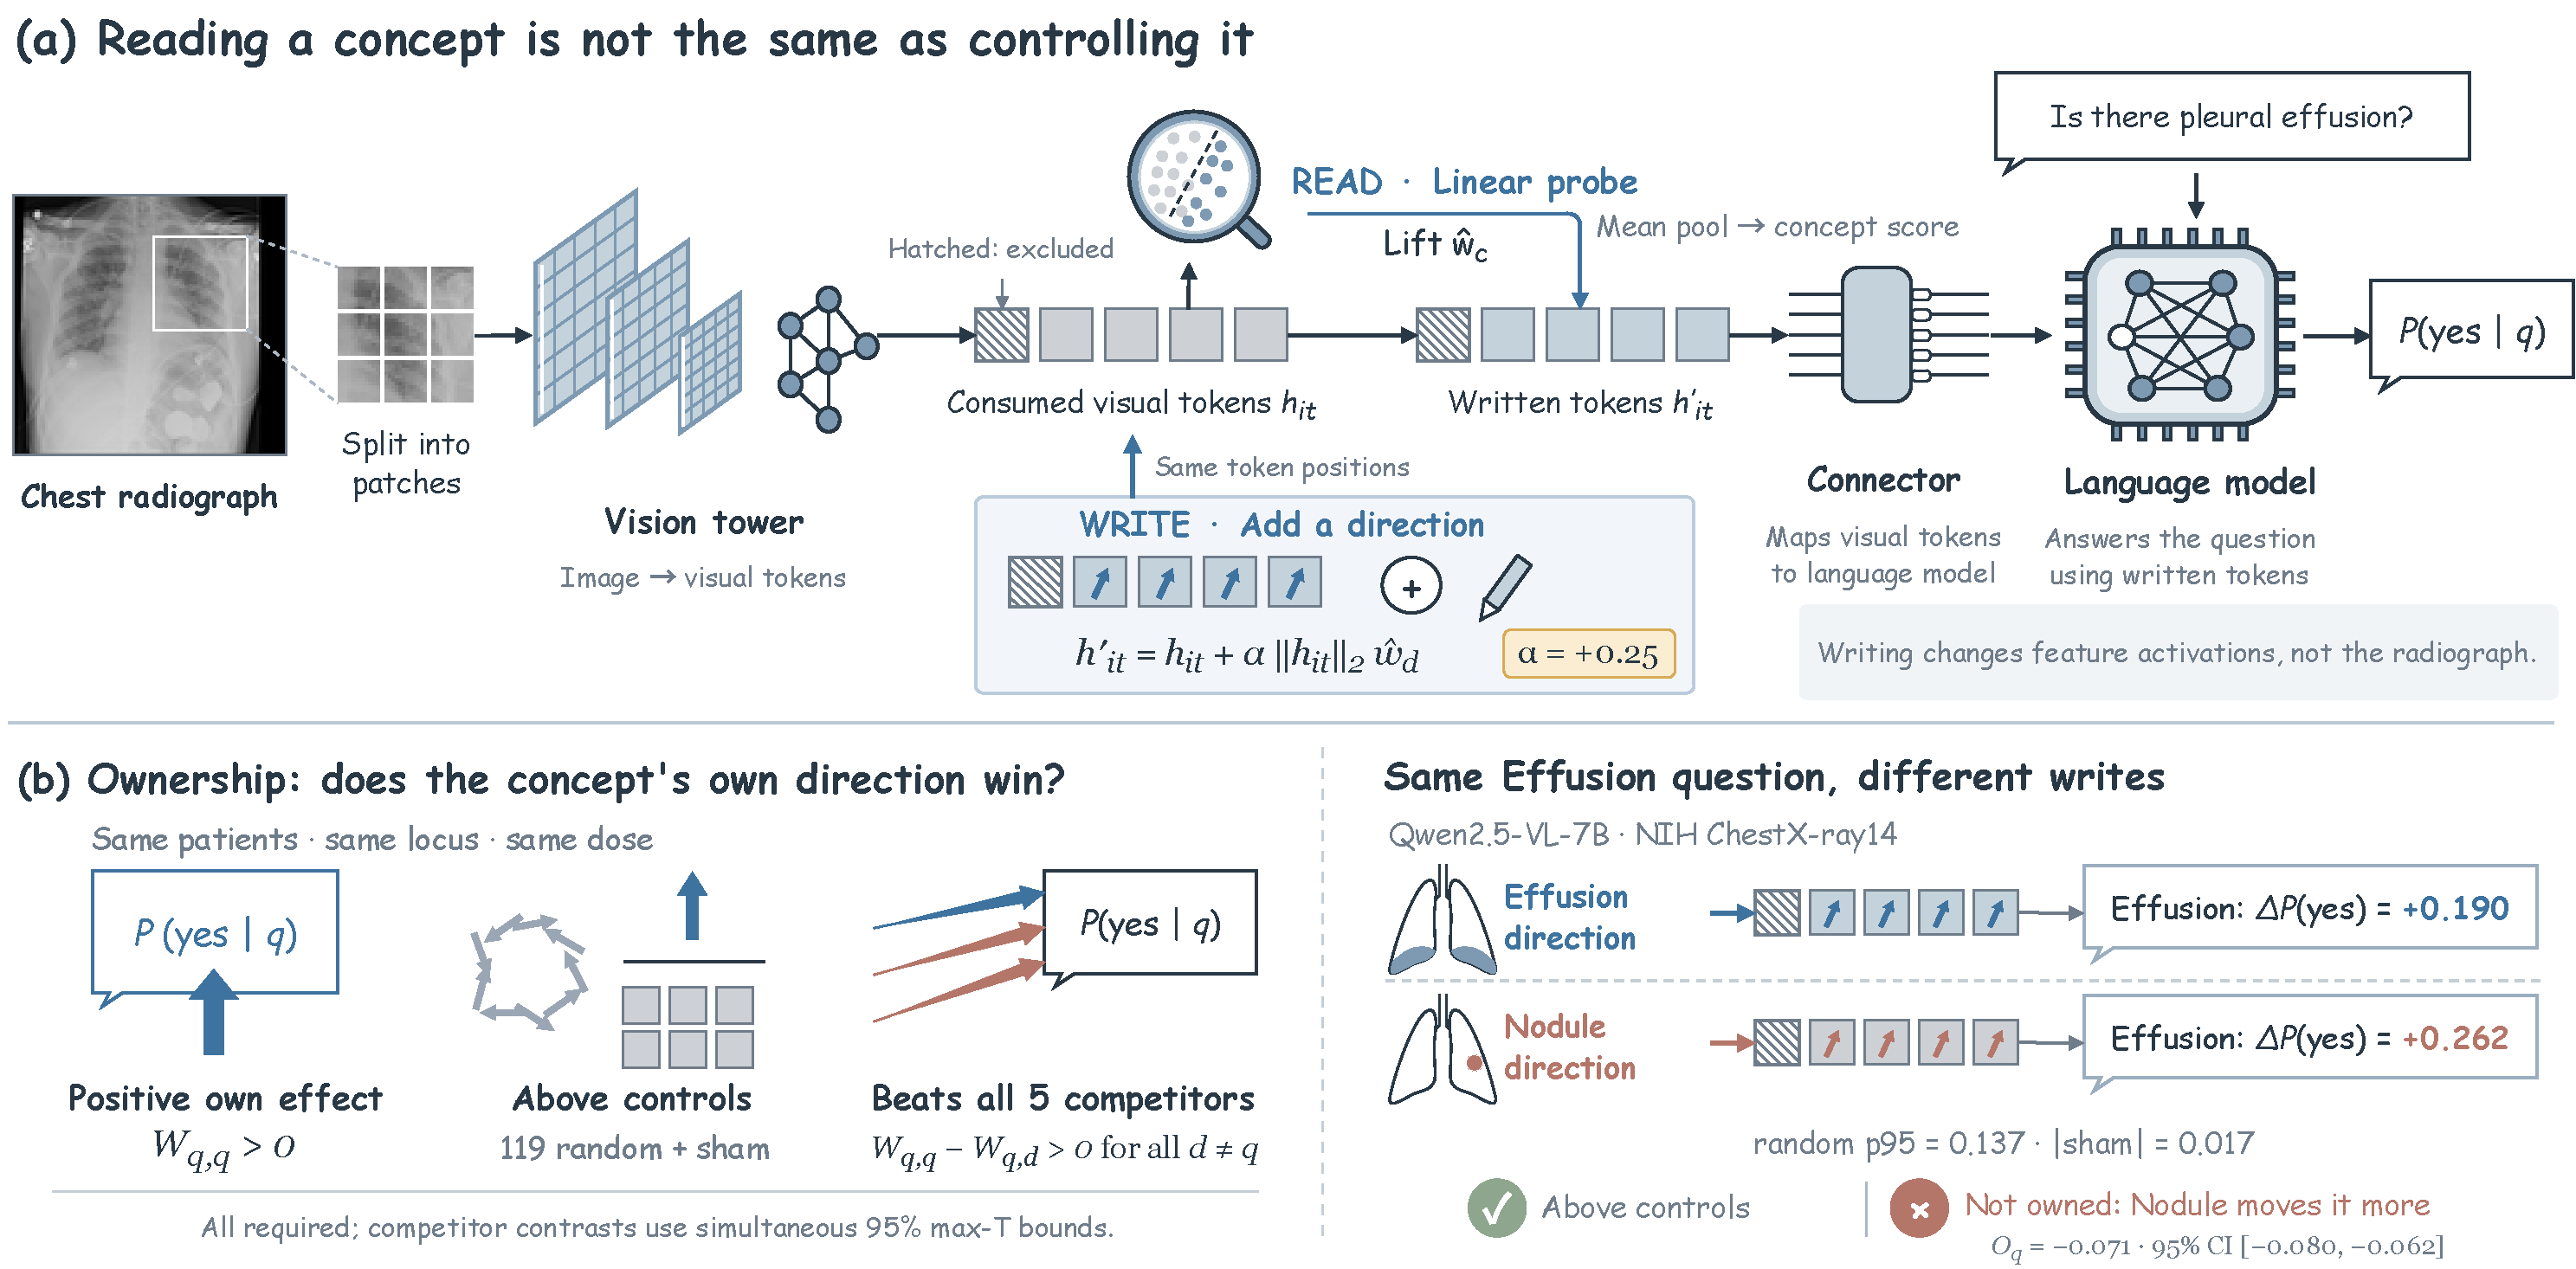
\includegraphics{figures/fig1_framework.pdf}}
    \caption{\textbf{Reading and writing a concept at the consumed block.} (a) The probe reads the concept from the consumed visual tokens, and its lifted normal is written back to them at dose $\alpha=+0.25$, a quarter of each token's norm. (b) Left: the three comparisons that decide ownership, on the write matrix $W_{q,d}$, the mean change in $P(\mathrm{yes})$ of question $q$ under a write along direction $d$. Right: the Effusion case (Qwen2.5-VL-7B, NIH ChestX-ray14): a stronger competitor.}
    \label{fig:framework}
\end{figure}

\paragraph{Contributions.} (i) We introduce ownership, which separates reading a concept from writing it: a probe direction is scored against directions fitted the same way for the competing concepts, written at the same locus and dose in the same patients (Section~\ref{sec:framework}). (ii) We identify the attribution deficit: across \cfCells{} checkpoint--concept cells, clinical concepts on chest radiographs are read and answered far more often than they are owned, and the gap to natural-image objects persists at matched answer ability (Sections~\ref{sec:headline}--\ref{sec:coco}). (iii) We trace the deficit to how the model reads the chest-radiograph representation rather than to the concept's clinical status, and show that a direction fitted to the model's own answers provides the handle that the label direction lacks (Sections~\ref{sec:reader}--\ref{sec:ansdir}). We release the evaluation, scorecards, and write matrices; a new model needs one adapter naming its consumed block.


\section{Background and Related Work}
\label{sec:related}

\paragraph{Probing and its controls.}
Linear probes track information across network depth \citep{alain2017understanding}, and a probe score reflects both the representation and the learner fitted to it, which motivates matched-capacity probes and control tasks \citep{hewitt2019designing}. The probing literature distinguishes information a readout can recover from information the model uses \citep{belinkov2022probing,ravichander2021probing}; causal erasure tests use by deleting a concept \citep{ravfogel2020null,elazar2021amnesic}, in closed form for every linear reader at once \citep{belrose2023leace}. Our readability grade adopts the control-task idea, and the write test asks a question complementary to erasure: whether the concept's own direction is the one that moves its answer. In medical multimodal models, depth-wise probing maps classification information across towers, connectors, and language layers \citep{zhu2026lost}, and layer-wise probes of MedCLIP expose acquisition and device shortcuts \citep{pedersen2026probes}; we intervene on the decoded clinical direction at the locus where it is read.

\paragraph{Concept directions and steering.}
A concept activation vector is the normal of a classifier separating concept examples from a negative set, and it grades a class by the directional derivative of the logit along that normal \citep{kim2018tcav}; we write the direction forward instead. Such a normal shifts with the layer it is fitted at, entangles with correlated concepts, depends on its negative set, and carries where in the image the concept was read \citep{nicolson2025explaining}. Representation engineering and activation steering write a concept back by changing intermediate representations at inference time \citep{zou2023representation,turner2023steering,panickssery2024caa}, and a probe normal is an appealing intervention because it supplies a label and a signed vector from the same representation. A separability-trained vector can, however, absorb distractor signals and diverge from its concept \citep{pahde2025navigating}: a classifier's weights are a filter rather than the pattern they detect \citep{haufe2014interpretation}, mass-mean directions steer truth judgements better than logistic normals \citep{marks2024geometry}, and the features that identify a concept are largely not those that control the output \citep{arad2025saes}. Benchmarks accordingly score concept detection and steering as separate axes \citep{wu2025axbench}, and alignment search certifies a subspace as causal when it implements an interpretable variable \citep{geiger2024alignments}. These works judge a direction mainly against its own concept. Ownership fixes the estimator and varies the label instead: it asks whether a direction fitted the same way for another concept moves the same answer more. Section~\ref{sec:robust-geometry} runs alternative constructions, a second locus, and token-concentrated writes through this test.

\paragraph{Writing into a vision-language model.}
Image features are linearly decodable in a vision-language model's hidden layers, and targeted edits to them change downstream answers \citep{rajaram2025lineofsight}. Steering one sparse-autoencoder feature of the vision tower and asking the language model what it sees recovers what that feature encodes \citep{ferrando2026explain}; we start from the meaning, fit a direction to a clinical label, and ask whether the write keeps that label's selectivity against the other findings' directions. Causal probing of multimodal models intervenes on the language model's residual stream with difference-in-means vectors and scores each concept against its own effect \citep{deng2026causal}; we write the representation the language model consumes and score each concept against its competitors.


\section{Reading, Answering, and Writing at the Consumed Block}
\label{sec:framework}

We ask three questions about a concept $c$ in a checkpoint $M$ on a dataset with binary labels: whether $c$ is readable from the visual representation the language model consumes, whether $M$ answers the question about $c$, and whether writing $c$'s own direction moves $c$'s answer more than any alternative. A registered protocol fixes an estimator and a decision rule for each question (Appendix~\ref{app:cf-labels}).

\subsection{Consumed block and matched read--write positions}
\label{sec:locus}

Every VLM in the grid passes an image through a vision tower and hands a specific tensor to a connector or merger that produces the language model's inputs. The \emph{consumed block} is the last visual block whose output that consumer reads, restricted to the token positions the consumer actually uses (CLS or padding rows are excluded where the consumer drops them); the \emph{connector locus} is the consumer's output. Appendix~\ref{app:repro-loci} identifies the block for every family. For image $i$ and consumed token $t$, let $\hvec_{it}\in\R^D$ be the output of the consumed block, where $D$ is the tower's hidden width; mean pooling over the consumed tokens gives the read vector $\hvec_i$. A write adds the unit direction $\hat\wvec_c$ of concept $c$ (Section~\ref{sec:directions}) to the same tokens,
\begin{equation}
\hvec'_{it}=\hvec_{it}+\alpha\,\lVert\hvec_{it}\rVert_2\,\hat\wvec_c,
\label{eq:intervention}
\end{equation}
so that the dose $\alpha$ is a fraction of each token's own norm, comparable across families whose activation scales differ by orders of magnitude, and its sign selects the concept's positive or negative pole. Reading and writing therefore use the same representation and the same positions. The connector and the language model, everything downstream of the consumed block, form the \emph{reader} of that representation.

\subsection{Directions, controls, and the reference family}
\label{sec:directions}

Each concept is read by a linear probe on a shared 512-dimensional view of the representation. A fixed Gaussian matrix $R\in\R^{D\times512}$ maps the read vector to features $\boldsymbol x_i=R^{\top}\hvec_i$, which are standardised with training-row means and scales $\boldsymbol s$; an $\ell_2$-regularised logistic regression with coefficient vector $\boldsymbol\beta_c$ then scores concept $c$ (inverse regularisation strength 1, 2{,}000 iterations, three fit seeds). The probe's logit is thus an affine function of $\hvec_i$ whose gradient is $R\,\mathrm{diag}(\boldsymbol s)^{-1}\boldsymbol\beta_c$, and the write direction is that gradient at unit length,
\begin{equation}
\hat\wvec_c=\frac{\boldsymbol g_c}{\lVert\boldsymbol g_c\rVert_2},\qquad \boldsymbol g_c=R\,\mathrm{diag}(\boldsymbol s)^{-1}\boldsymbol\beta_c .
\label{eq:lift}
\end{equation}
It is the direction in the consumed representation along which the probe's evidence for $c$ grows fastest (Appendix~\ref{app:repro-probe} gives the numerical details). We call it the concept's \emph{label direction}, since it is fitted to the concept's labels.

Two families of controls bracket the label direction. For reading, 20 control probes are fitted to random labels drawn within recurring image types (view, sex, and age decade on chest sets; aspect and area buckets on COCO), so that they have the capacity and the nuisance structure of the concept probe. With $y$ the concept labels and $r$ the probe's scores on the calibration rows, and $y^{\mathrm{ctrl}}_k$ and $r^{\mathrm{ctrl}}_k$ the random labels and scores of control probe $k$, the probe's selectivity is
\begin{equation}
S=\operatorname{AUROC}(y,r)-\tfrac{1}{20}\textstyle\sum_{k=1}^{20}\operatorname{AUROC}(y^{\mathrm{ctrl}}_k,r^{\mathrm{ctrl}}_k),
\label{eq:selectivity}
\end{equation}
which is positive when the probe reads its concept better than a probe of equal capacity reads an arbitrary label with the same nuisance structure. For writing, the \emph{reference family} contains 119 random unit directions, a coordinate-permutation sham of $\hat\wvec_c$ (same coordinates, scrambled arrangement), and the five label directions of the other clinical concepts, all written at the same dose to the same images.

\subsection{Ownership}
\label{sec:ownership}

Each dataset has six concepts, and we index both the yes/no question about a concept and the direction fitted for it by that concept. For question $q$ and direction $d$, $W_{q,d}$ is the mean over test images of the change in $P(\mathrm{yes})$ for question $q$ when $\hat\wvec_d$ is written, each image scored with and without the write. Here $P(\mathrm{yes})=\sigma(\ell_{\mathrm{yes}}-\ell_{\mathrm{no}})$, where $\sigma$ is the logistic function and $\ell_{\mathrm{yes}}$ and $\ell_{\mathrm{no}}$ are the log-probabilities of the two answers at the first answer position, each the maximum over case and leading-space variants that tokenise to one token. Row $q$ of the $6\times6$ write matrix $W$ records how far each direction moves question $q$, and its diagonal entry $W_{q,q}$ is the concept's own write (Figure~\ref{fig:write-matrices}). Ownership is the diagonal margin
\begin{equation}
O_q=W_{q,q}-\max_{d\neq q}W_{q,d},
\label{eq:margin}
\end{equation}
the advantage of the concept's own direction over its strongest clinical competitor on the concept's own question. $W_{q,q}$ measures how far the concept's own direction moves its answer; $O_q$ measures whether it moves that answer further than every competitor built the same way. A large $W_{q,q}$ shows that $d=q$ can write the answer; only $O_q>0$ shows that the label names the effective direction. A concept can therefore fail ownership in two ways: its own write stays within the random and sham references, or the write clears them without holding its advantage over every competitor. Section~\ref{sec:headline} measures both. The Effusion case of the introduction illustrates the latter: the Effusion direction raises the Effusion answer by $\cfSeedWEff$, above the random 95th percentile and the sham, and the Nodule direction raises the same answer by $\cfSeedWNodule$, so $O_{\mathrm{Effusion}}=\cfSeedEffO$. Uncertainty over patients comes from 2{,}000 bootstrap draws of test rows, with the maximum in Equation~\ref{eq:margin} recomputed inside every draw. The 30 contrasts $W_{q,q}-W_{q,d}$ (six questions, five competitors each) receive simultaneous 95\% bounds from a centred studentised max-$T$ bootstrap, which hold jointly across all 30 (Appendix~\ref{app:simultaneous-bounds}).

\subsection{Graded outcomes}
\label{sec:grades}

The readable and answerable grades are computed on the 400 calibration rows, which carry no write. The write matrix and every ownership quantity are computed on the 600 test rows, which share no patient with the calibration rows.
\begin{itemize}[leftmargin=*,itemsep=1pt,topsep=2pt]
\item \textbf{Readable:} the one-sided 95\% lower bound of $S$ on the calibration rows is above zero, with at least ten known positives and ten known negatives among those 400 rows.
\item \textbf{Answerable:} the \emph{clean answer}, $P(\mathrm{yes})$ with no write, separates the concept's labels: the one-sided 95\% lower bound of its AUROC on the same calibration rows is above $0.5$, under the same ten-and-ten support rule.
\item \textbf{Owned:} on the test rows, the write meets the \emph{steering reference} ($W_{q,q}>0$, above the 95th percentile of the 119 random writes, and above the sham's absolute effect) and every simultaneous lower bound of $W_{q,q}-W_{q,d}$ is positive. A cell with any simultaneous upper bound below zero has a \emph{stronger competitor}; the rest are \emph{unresolved}.
\end{itemize}
A checkpoint--concept pair on one dataset is a \emph{cell}, and a checkpoint--dataset pair is a \emph{block}. A cell graded owned is said to be owned, and the checkpoint is said to own the concept; an alternative direction is owned in a cell when its write meets the same rule for that concept. A block contributes to the answerable and owned counts only when its write matrix and its calibration pass both completed. The grades are defined for one direction construction, one primary dose with a five-point sweep, six templates, pooled consumed-token features, and two loci, the consumed block and the connector output. Before a block is scored, seven acceptance checks on 16 held-out preflight rows confirm, at both loci, that scoring is deterministic, that $\alpha=0$ changes nothing, that the write reaches the answer and changes nothing outside the consumed tokens, and that every template maps its answers correctly without an image (Appendix~\ref{app:cf-gates}).
\label{sec:gates}


\section{Models, Datasets, and Scale}
\label{sec:setup}

\paragraph{Checkpoints.}
We evaluate \cfCheckpoints{} instruction-tuned checkpoints from \cfFamiliesWord{} families, 3B to 72B (Table~\ref{tab:cf-models}). Six families are general-purpose: Qwen2.5-VL \citep{bai2025qwen25vl}, Qwen3-VL \citep{qwen2025qwen3vl}, InternVL3.5 \citep{wang2025internvl35}, Gemma~3 \citep{gemma2025gemma3}, LLaVA-1.5 \citep{liu2024improved}, and Llama~3.2~Vision \citep{meta2024llama32vision}. Six are medical fine-tunes: MedGemma \citep{sellergren2025medgemma}, Lingshu \citep{lasa2025lingshu}, LLaVA-Med~1.5 \citep{li2023llavamed}, CheXagent \citep{chen2024chexagent}, HuatuoGPT-Vision \citep{chen2024huatuogptvision}, and LLaVA-Rad \citep{zambranochaves2025llavarad}. They span \cfTowerDesignsWord{} vision-tower designs and three consumer designs: token insertion after a merger, token insertion after a projector, and cross-attention. Three towers are trained on chest radiographs, those of CheXagent-2-3B, CheXagent-8B, and LLaVA-Rad-7B (Appendix~\ref{app:cf-grid}). Every checkpoint runs in bf16 with its native processor.

\paragraph{Datasets and cohorts.}
NIH ChestX-ray14 \citep{wang2017chestxray} and CheXpert Plus \citep{chambon2024chexpertplus} provide frontal chest radiographs with report-derived labels, the CheXpert labels coming from the CheXpert labeler \citep{irvin2019chexpert}. We evaluate six findings per dataset (NIH: Effusion, Atelectasis, Pneumothorax, Cardiomegaly, Mass, Nodule; CheXpert: Effusion, Atelectasis, Pneumothorax, Cardiomegaly, Consolidation, Edema). COCO \citep{lin2014coco} provides the natural-image control, with binary presence labels for six object categories (person, dog, car, chair, bottle, bicycle). Seeded hashes of patient or image identity select one fixed cohort per dataset, shared by every checkpoint: 20{,}000 training rows (\cfCohortNihTrainRows{} on NIH) fit the probes and the answer direction, 400 calibration rows carry the readable and answerable grades, 600 test rows carry every write, and 16 preflight rows carry the acceptance checks. No patient and no image appears in two roles of a dataset (Appendix~\ref{app:repro-cohorts}).

\paragraph{Questions and scale.}
Each concept is asked as a yes/no question in six templates that cross two wordings (\emph{is there} versus \emph{does the image show}) with three answer interfaces (yes/no, A-present, B-present); the \emph{is}/yes-no template gives the primary grade (Appendix~\ref{app:protocol}). The primary dose is $\alpha=+0.25$, and a sweep adds $\alpha\in\{-0.5,-0.25,-0.1,+0.1,+0.5\}$. Each block scores the write matrix, the sham, and the 119 random directions on the 600 test rows. The campaign comprises \cfBlocks{} blocks, \cfCells{} scored concept cells, about 30 million scored answers, and roughly 3{,}000 A100-hours; \cfCoverageBlocksAllSeven{} of the \cfBlocks{} blocks carry every planned analysis (Appendix~\ref{app:cf-coverage}).


\section{Results}
\label{sec:results}

\subsection{Reading is not writing}
\label{sec:headline}

On both chest datasets, reading and answering far outpace writing (Table~\ref{tab:cf-main}, Figure~\ref{fig:overview}a--b). Clinical concepts are readable in \cfChestReadable{} of \cfChestReadableN{} cells (\cfChestReadablePct\%; median selectivity $\cfSelChestMed$), and \cfChestAnswerable{} (\cfChestAnswerablePct\%) are answerable. Yet only \cfChestOwned{} cells (\cfChestOwnedPct\%) are owned, and reading and answering together barely change this: \cfReadAnsOwned{} of the \cfReadAns{} readable and answerable cells are owned (\cfReadAnsOwnedPct\%), against \cfRestOwned{} of the remaining \cfRestN{} (\cfRestOwnedPct\%).

Ownership on chest radiographs breaks at the write itself. \cfChestRefBelow{} of \cfChestCellsN{} label directions fail the random and sham reference for their own question, and these cells carry \cfChestBelowStrong{} of the \cfChestCompetitor{} stronger-competitor verdicts (\cfChestBelowStrongPct\%). Once an own write clears the reference, \cfChestOwned{} of \cfChestRefMet{} cells are owned; on COCO, \cfCocoRefMet{} of \cfCocoOwnedN{} writes clear it and \cfCocoOwned{} are owned. On chest radiographs, most label directions therefore scarcely move the answers they name, while the directions of other findings often move those answers more.

\label{sec:seed}The Effusion case reproduces on 600 new patients (Table~\ref{tab:cf-seed}). The Effusion write raises its answer by $\cfSeedWEff$, second among the 120 compared effects, the Nodule write raises it by $\cfSeedWNodule$, and $O_{\mathrm{Effusion}}=\cfSeedEffO$ $[\cfSeedEffOLo,\cfSeedEffOHi]$, matching the $\cfSeedPriorO$ $[\cfSeedPriorOLo,\cfSeedPriorOHi]$ of the two-model pilot study that motivated the evaluation (Appendix~\ref{app:seed}). Across the grid, Effusion is owned in \cfEffusionOwnedBlocks{} of \cfChestBlocks{} chest blocks, and in \cfEffusionOwnedSmall{} of these $O_{\mathrm{Effusion}}\leq0.03$.

\begin{table}[t]
\centering
\setlength{\tabcolsep}{2pt}
\renewcommand{\arraystretch}{1.08}
% terracotta = positive / high, blue = negative / low, sage = magnitude of Read and Ans; darker = larger magnitude
\definecolor{cfSage1}{HTML}{ECF3EF}
\definecolor{cfSage2}{HTML}{D5E5DB}
\definecolor{cfSage3}{HTML}{B9D4C3}
\definecolor{cfSage4}{HTML}{9EC3AC}
\definecolor{cfSlate1}{HTML}{EAF0F6}
\definecolor{cfSlate2}{HTML}{D0DDEA}
\definecolor{cfSlate3}{HTML}{B1C7DD}
\definecolor{cfSlate4}{HTML}{94B2D0}
\definecolor{cfTerra1}{HTML}{F7ECEA}
\definecolor{cfTerra2}{HTML}{EED5D1}
\definecolor{cfTerra3}{HTML}{E2B8B2}
\definecolor{cfTerra4}{HTML}{D79E95}
\definecolor{cfOat1}{HTML}{F4EFE6}
\definecolor{cfOat2}{HTML}{E8DDC8}
\definecolor{cfGrey}{HTML}{E4E1DC}

\caption{\textbf{Reading, answering, and writing per checkpoint.} Per dataset: mean probe selectivity $S$ (\textsc{Read}), mean clean-answer AUROC (\textsc{Ans}), and mean ownership $O_q$ (\textsc{Own}), each superscripted with the number of the six concepts that receive the grade; then the owned share of clinical and COCO cells and their ratio, by which rows are sorted. Shading darkens with magnitude (blue for negative \textsc{Own}); ``--'' marks an undefined ratio.}
\label{tab:cf-main}
\resizebox{\linewidth}{!}{%
\begin{tabular}{l@{\hspace{3pt}}ccc@{\hspace{4pt}}ccc@{\hspace{4pt}}ccc@{\hspace{4pt}}ccc}
\toprule
\multirow{2}{*}{Checkpoint} & \multicolumn{3}{c}{NIH ChestX-ray14} & \multicolumn{3}{c}{CheXpert Plus} & \multicolumn{3}{c}{COCO (control)} & \multicolumn{3}{c}{Owned share}\\
\cmidrule(lr){2-4}\cmidrule(lr){5-7}\cmidrule(lr){8-10}\cmidrule(lr){11-13}
& \multicolumn{1}{c}{\textsc{Read}} & \multicolumn{1}{c}{\textsc{Ans}} & \multicolumn{1}{c}{\textsc{Own}} & \multicolumn{1}{c}{\textsc{Read}} & \multicolumn{1}{c}{\textsc{Ans}} & \multicolumn{1}{c}{\textsc{Own}} & \multicolumn{1}{c}{\textsc{Read}} & \multicolumn{1}{c}{\textsc{Ans}} & \multicolumn{1}{c}{\textsc{Own}} & \multicolumn{1}{c}{clin.} & \multicolumn{1}{c}{COCO} & \multicolumn{1}{c}{ratio}\\
\midrule
Lingshu 32B & \cellcolor{cfSage2}0.08$^{3}$ & \cellcolor{cfSage3}0.78$^{6}$ & \cellcolor{cfSlate2}-0.02$^{2}$ & \cellcolor{cfSage4}0.20$^{4}$ & \cellcolor{cfSage3}0.87$^{5}$ & \cellcolor{cfTerra2}+0.04$^{5}$ & \cellcolor{cfSage1}0.03$^{1}$ & \cellcolor{cfSage4}0.95$^{5}$ & \cellcolor{cfTerra4}+0.28$^{6}$ & \cellcolor{cfTerra4}58\% & \cellcolor{cfTerra4}100\% & 58\% \\
CheXagent-2-3B & \cellcolor{cfSage3}0.13$^{5}$ & \cellcolor{cfSage3}0.86$^{6}$ & \cellcolor{cfTerra1}+0.00$^{2}$ & \cellcolor{cfSage4}0.21$^{5}$ & \cellcolor{cfSage4}0.95$^{5}$ & \cellcolor{cfTerra1}+0.01$^{4}$ & \cellcolor{cfSage3}0.13$^{4}$ & \cellcolor{cfSage3}0.81$^{5}$ & \cellcolor{cfTerra2}+0.03$^{2}$ & \cellcolor{cfTerra4}50\% & \cellcolor{cfTerra2}33\% & 150\% \\
Qwen2.5-VL-72B & \cellcolor{cfSage2}0.07$^{2}$ & \cellcolor{cfSage2}0.62$^{4}$ & \cellcolor{cfSlate2}-0.03$^{3}$ & \cellcolor{cfSage3}0.20$^{4}$ & \cellcolor{cfSage2}0.71$^{4}$ & \cellcolor{cfSlate2}-0.09$^{1}$ & \cellcolor{cfSage1}0.01$^{1}$ & \cellcolor{cfSage4}0.99$^{5}$ & \cellcolor{cfTerra4}+0.66$^{6}$ & \cellcolor{cfTerra3}33\% & \cellcolor{cfTerra4}100\% & 33\% \\
Lingshu 7B & \cellcolor{cfSage2}0.08$^{3}$ & \cellcolor{cfSage3}0.76$^{6}$ & \cellcolor{cfTerra2}+0.02$^{1}$ & \cellcolor{cfSage4}0.21$^{4}$ & \cellcolor{cfSage3}0.86$^{5}$ & \cellcolor{cfTerra2}+0.04$^{3}$ & \cellcolor{cfSage1}0.02$^{1}$ & \cellcolor{cfSage4}0.97$^{5}$ & \cellcolor{cfTerra4}+0.68$^{6}$ & \cellcolor{cfTerra3}33\% & \cellcolor{cfTerra4}100\% & 33\% \\
Qwen3-VL-4B & \cellcolor{cfSage2}0.08$^{3}$ & \cellcolor{cfSage2}0.71$^{6}$ & \cellcolor{cfSlate3}-0.11$^{0}$ & \cellcolor{cfSage4}0.20$^{4}$ & \cellcolor{cfSage2}0.74$^{4}$ & \cellcolor{cfSlate1}-0.01$^{2}$ & \cellcolor{cfSage1}0.04$^{4}$ & \cellcolor{cfSage4}0.99$^{5}$ & \cellcolor{cfTerra4}+0.34$^{6}$ & \cellcolor{cfTerra3}17\% & \cellcolor{cfTerra4}100\% & 17\% \\
Qwen3-VL-32B & \cellcolor{cfSage2}0.10$^{2}$ & \cellcolor{cfSage2}0.70$^{6}$ & \cellcolor{cfSlate2}-0.02$^{1}$ & \cellcolor{cfSage3}0.17$^{5}$ & \cellcolor{cfSage3}0.82$^{5}$ & \cellcolor{cfSlate2}-0.02$^{1}$ & \cellcolor{cfSage2}0.05$^{4}$ & \cellcolor{cfSage4}0.99$^{5}$ & \cellcolor{cfTerra3}+0.15$^{6}$ & \cellcolor{cfTerra3}17\% & \cellcolor{cfTerra4}100\% & 17\% \\
InternVL3.5-38B & \cellcolor{cfSage2}0.10$^{5}$ & \cellcolor{cfSage3}0.78$^{6}$ & \cellcolor{cfSlate1}-0.00$^{0}$ & \cellcolor{cfSage3}0.17$^{4}$ & \cellcolor{cfSage3}0.86$^{5}$ & \cellcolor{cfSlate1}-0.00$^{2}$ & \cellcolor{cfSage2}0.08$^{4}$ & \cellcolor{cfSage4}0.99$^{5}$ & \cellcolor{cfTerra1}+0.01$^{6}$ & \cellcolor{cfTerra3}17\% & \cellcolor{cfTerra4}100\% & 17\% \\
Gemma 3 12B & \cellcolor{cfSage2}0.07$^{2}$ & \cellcolor{cfSage2}0.62$^{5}$ & \cellcolor{cfSlate4}-0.37$^{1}$ & \cellcolor{cfSage3}0.18$^{4}$ & \cellcolor{cfSage1}0.52$^{0}$ & \cellcolor{cfSlate4}-0.38$^{1}$ & \cellcolor{cfSage2}0.07$^{5}$ & \cellcolor{cfSage4}0.95$^{5}$ & \cellcolor{cfTerra4}+0.44$^{6}$ & \cellcolor{cfTerra3}17\% & \cellcolor{cfTerra4}100\% & 17\% \\
MedGemma 4B & \cellcolor{cfSage3}0.12$^{3}$ & \cellcolor{cfSage3}0.80$^{6}$ & \cellcolor{cfSlate3}-0.13$^{0}$ & \cellcolor{cfSage4}0.21$^{4}$ & \cellcolor{cfSage3}0.87$^{5}$ & \cellcolor{cfSlate3}-0.16$^{2}$ & \cellcolor{cfSage2}0.06$^{4}$ & \cellcolor{cfSage4}0.94$^{5}$ & \cellcolor{cfTerra3}+0.23$^{6}$ & \cellcolor{cfTerra3}17\% & \cellcolor{cfTerra4}100\% & 17\% \\
InternVL3.5-14B & \cellcolor{cfSage2}0.07$^{4}$ & \cellcolor{cfSage2}0.73$^{6}$ & \cellcolor{cfSlate1}-0.00$^{1}$ & \cellcolor{cfSage3}0.16$^{4}$ & \cellcolor{cfSage3}0.87$^{5}$ & \cellcolor{cfTerra1}+0.00$^{1}$ & \cellcolor{cfSage3}0.12$^{4}$ & \cellcolor{cfSage4}0.98$^{5}$ & \cellcolor{cfTerra1}+0.02$^{5}$ & \cellcolor{cfTerra3}17\% & \cellcolor{cfTerra3}83\% & 20\% \\
Qwen2.5-VL-32B & \cellcolor{cfSage2}0.09$^{3}$ & \cellcolor{cfSage2}0.63$^{4}$ & \cellcolor{cfSlate2}-0.06$^{1}$ & \cellcolor{cfSage3}0.16$^{4}$ & \cellcolor{cfSage2}0.70$^{4}$ & \cellcolor{cfSlate3}-0.11$^{0}$ & \cellcolor{cfSage1}0.02$^{1}$ & \cellcolor{cfSage4}0.99$^{5}$ & \cellcolor{cfTerra4}+0.38$^{6}$ & \cellcolor{cfTerra2}8\% & \cellcolor{cfTerra4}100\% & 8\% \\
InternVL3.5-8B & \cellcolor{cfSage2}0.06$^{2}$ & \cellcolor{cfSage2}0.73$^{6}$ & \cellcolor{cfSlate1}-0.01$^{0}$ & \cellcolor{cfSage3}0.19$^{4}$ & \cellcolor{cfSage3}0.86$^{5}$ & \cellcolor{cfSlate1}-0.00$^{1}$ & \cellcolor{cfSage2}0.12$^{5}$ & \cellcolor{cfSage4}0.98$^{5}$ & \cellcolor{cfTerra2}+0.03$^{6}$ & \cellcolor{cfTerra2}8\% & \cellcolor{cfTerra4}100\% & 8\% \\
HuatuoGPT-Vision-7B & \cellcolor{cfSage2}0.08$^{3}$ & \cellcolor{cfSage2}0.71$^{6}$ & \cellcolor{cfSlate2}-0.03$^{1}$ & \cellcolor{cfSage3}0.19$^{4}$ & \cellcolor{cfSage3}0.78$^{4}$ & \cellcolor{cfSlate1}-0.01$^{0}$ & \cellcolor{cfSage2}0.07$^{4}$ & \cellcolor{cfSage4}0.99$^{5}$ & \cellcolor{cfTerra1}+0.01$^{4}$ & \cellcolor{cfTerra2}8\% & \cellcolor{cfTerra3}67\% & 12\% \\
LLaVA-Med 1.5 7B & \cellcolor{cfSage2}0.08$^{3}$ & \cellcolor{cfSage1}0.53$^{0}$ & \cellcolor{cfSlate1}-0.01$^{0}$ & \cellcolor{cfSage3}0.19$^{4}$ & \cellcolor{cfSage1}0.59$^{2}$ & \cellcolor{cfSlate1}-0.01$^{1}$ & \cellcolor{cfSage2}0.07$^{4}$ & \cellcolor{cfSage3}0.76$^{5}$ & \cellcolor{cfTerra1}+0.00$^{1}$ & \cellcolor{cfTerra2}8\% & \cellcolor{cfTerra2}17\% & 50\% \\
CheXagent-8B & \cellcolor{cfSage3}0.16$^{5}$ & \cellcolor{cfSage2}0.73$^{6}$ & \cellcolor{cfSlate1}-0.00$^{0}$ & \cellcolor{cfSage4}0.23$^{5}$ & \cellcolor{cfSage3}0.88$^{5}$ & \cellcolor{cfSlate1}-0.02$^{1}$ & \cellcolor{cfSage2}0.05$^{3}$ & \cellcolor{cfSage1}0.52$^{1}$ & \cellcolor{cfSlate2}-0.03$^{0}$ & \cellcolor{cfTerra2}8\% & \cellcolor{cfTerra1}0\% & -- \\
Qwen2.5-VL-3B & \cellcolor{cfSage2}0.07$^{2}$ & \cellcolor{cfSage1}0.58$^{2}$ & \cellcolor{cfSlate2}-0.08$^{0}$ & \cellcolor{cfSage3}0.17$^{4}$ & \cellcolor{cfSage1}0.57$^{2}$ & \cellcolor{cfSlate2}-0.07$^{0}$ & \cellcolor{cfSage1}0.05$^{4}$ & \cellcolor{cfSage4}0.97$^{5}$ & \cellcolor{cfTerra4}+0.52$^{6}$ & \cellcolor{cfTerra1}0\% & \cellcolor{cfTerra4}100\% & 0\% \\
Qwen2.5-VL-7B & \cellcolor{cfSage2}0.08$^{3}$ & \cellcolor{cfSage2}0.62$^{3}$ & \cellcolor{cfSlate3}-0.14$^{0}$ & \cellcolor{cfSage3}0.20$^{4}$ & \cellcolor{cfSage2}0.65$^{2}$ & \cellcolor{cfSlate2}-0.08$^{0}$ & \cellcolor{cfSage1}0.02$^{1}$ & \cellcolor{cfSage4}0.98$^{5}$ & \cellcolor{cfTerra4}+0.67$^{6}$ & \cellcolor{cfTerra1}0\% & \cellcolor{cfTerra4}100\% & 0\% \\
Qwen3-VL-8B & \cellcolor{cfSage2}0.10$^{4}$ & \cellcolor{cfSage2}0.69$^{6}$ & \cellcolor{cfSlate1}-0.01$^{0}$ & \cellcolor{cfSage3}0.17$^{4}$ & \cellcolor{cfSage2}0.75$^{4}$ & \cellcolor{cfSlate2}-0.04$^{0}$ & \cellcolor{cfSage1}0.04$^{3}$ & \cellcolor{cfSage4}0.99$^{5}$ & \cellcolor{cfTerra4}+0.58$^{6}$ & \cellcolor{cfTerra1}0\% & \cellcolor{cfTerra4}100\% & 0\% \\
Gemma 3 27B & \cellcolor{cfSage2}0.07$^{2}$ & \cellcolor{cfSage2}0.60$^{3}$ & \cellcolor{cfSlate2}-0.03$^{0}$ & \cellcolor{cfSage3}0.18$^{4}$ & \cellcolor{cfSage1}0.55$^{2}$ & \cellcolor{cfSlate1}-0.01$^{0}$ & \cellcolor{cfSage2}0.07$^{5}$ & \cellcolor{cfSage4}0.96$^{5}$ & \cellcolor{cfTerra4}+0.31$^{6}$ & \cellcolor{cfTerra1}0\% & \cellcolor{cfTerra4}100\% & 0\% \\
Gemma 3 4B & \cellcolor{cfSage2}0.07$^{2}$ & \cellcolor{cfSage1}0.56$^{2}$ & \cellcolor{cfSlate3}-0.11$^{0}$ & \cellcolor{cfSage3}0.18$^{4}$ & \cellcolor{cfSage1}0.53$^{1}$ & \cellcolor{cfSlate4}-0.27$^{0}$ & \cellcolor{cfSage2}0.07$^{5}$ & \cellcolor{cfSage4}0.94$^{5}$ & \cellcolor{cfTerra3}+0.24$^{5}$ & \cellcolor{cfTerra1}0\% & \cellcolor{cfTerra3}83\% & 0\% \\
LLaVA-1.5-7B & \cellcolor{cfSage2}0.08$^{2}$ & \cellcolor{cfSage1}0.51$^{0}$ & \cellcolor{cfSlate2}-0.04$^{0}$ & \cellcolor{cfSage3}0.17$^{4}$ & \cellcolor{cfSage1}0.52$^{0}$ & \cellcolor{cfSlate2}-0.03$^{0}$ & \cellcolor{cfSage4}0.28$^{5}$ & \cellcolor{cfSage4}0.97$^{5}$ & \cellcolor{cfTerra2}+0.03$^{5}$ & \cellcolor{cfTerra1}0\% & \cellcolor{cfTerra3}83\% & 0\% \\
MedGemma 27B & \cellcolor{cfSage3}0.12$^{3}$ & \cellcolor{cfSage3}0.80$^{6}$ & \cellcolor{cfSlate3}-0.14$^{0}$ & \cellcolor{cfSage4}0.21$^{4}$ & \cellcolor{cfSage3}0.87$^{5}$ & \cellcolor{cfSlate2}-0.06$^{0}$ & \cellcolor{cfSage2}0.06$^{4}$ & \cellcolor{cfSage4}0.97$^{5}$ & \cellcolor{cfTerra3}+0.12$^{4}$ & \cellcolor{cfTerra1}0\% & \cellcolor{cfTerra3}67\% & 0\% \\
LLaVA-1.5-13B & \cellcolor{cfSage2}0.08$^{2}$ & \cellcolor{cfSage1}0.53$^{0}$ & \cellcolor{cfSlate2}-0.02$^{0}$ & \cellcolor{cfSage3}0.17$^{4}$ & \cellcolor{cfSage1}0.51$^{1}$ & \cellcolor{cfSlate1}-0.01$^{0}$ & \cellcolor{cfSage4}0.28$^{5}$ & \cellcolor{cfSage4}0.96$^{5}$ & \cellcolor{cfTerra2}+0.02$^{2}$ & \cellcolor{cfTerra1}0\% & \cellcolor{cfTerra2}33\% & 0\% \\
Llama 3.2 Vision 11B & \cellcolor{cfSage2}0.08$^{2}$ & \cellcolor{cfSage2}0.65$^{4}$ & \cellcolor{cfSlate2}-0.03$^{0}$ & \cellcolor{cfSage3}0.16$^{4}$ & \cellcolor{cfSage2}0.73$^{4}$ & \cellcolor{cfSlate2}-0.04$^{0}$ & \cellcolor{cfSage3}0.12$^{5}$ & \cellcolor{cfSage4}0.95$^{5}$ & \cellcolor{cfSlate1}-0.01$^{1}$ & \cellcolor{cfTerra1}0\% & \cellcolor{cfTerra2}17\% & 0\% \\
LLaVA-Rad-7B & \cellcolor{cfSage3}0.15$^{4}$ & \cellcolor{cfSage2}0.71$^{5}$ & \cellcolor{cfSlate1}-0.01$^{0}$ & \cellcolor{cfSage4}0.27$^{5}$ & \cellcolor{cfSage3}0.87$^{5}$ & \cellcolor{cfSlate1}-0.02$^{0}$ & \cellcolor{cfSage3}0.12$^{4}$ & \cellcolor{cfSage1}0.50$^{0}$ & \cellcolor{cfSlate2}-0.03$^{0}$ & \cellcolor{cfTerra1}0\% & \cellcolor{cfTerra1}0\% & -- \\
\midrule
\textbf{All cells} & 0.09 & 0.68 & -0.06 & 0.19 & 0.74 & -0.05 & 0.08 & 0.92 & +0.23 & 13\% & 75\% & 17\% \\
\quad count / cells & 74/150 & 110/150 & 13/150 & 104/150 & 89/150 & 25/150 & 90/150 & 116/150 & 113/150 & & & \\
\bottomrule
\end{tabular}}
\end{table}


\begin{figure}[t]
    \centering
    \resizebox{\textwidth}{!}{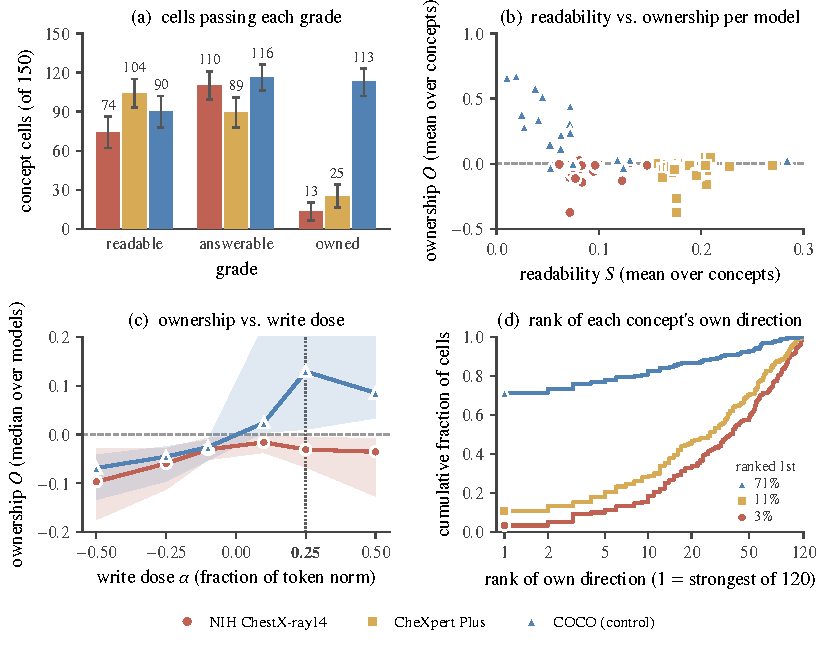
\includegraphics{figures/fig2_overview.pdf}}
    \caption{\textbf{Reading, answering, and writing across the grid.} (a) Readable, answerable, and owned cells of 150 per dataset, with descriptive 95\% bootstrap intervals over cells. (b) Mean readability against mean ownership per checkpoint. (c) Median ownership and interquartile band over 25 blocks against the dose; the dotted line marks the graded dose $\alpha=+0.25$, and the COCO band is clipped at $0.2$. (d) Cumulative share of cells by the rank of the concept write among the 120 compared effects.}
    \label{fig:overview}
\end{figure}

\subsection{Where the chest write goes}
\label{sec:deficit}

Clinical writes are not selective (Figure~\ref{fig:write-flow}). The written concept's own question receives \cfOwnShareNih\% of the positive answer change on NIH and \cfOwnShareChex\% on CheXpert, against \cfOwnShareCoco\% on COCO. The write matrices show the same structure (Figure~\ref{fig:write-matrices}). The own write is small, with median $W_{q,q}$ of $\cfMedianWqqNih$ on NIH and $\cfMedianWqqChex$ on CheXpert against $\cfMedianWqqCoco$ on COCO, and the competing directions share what effect there is: the Atelectasis, Effusion, and Consolidation directions raise each other's answers by similar amounts, and on the chest sets a row of $W$ is flat or peaks off the diagonal, whereas on COCO the diagonal dominates. At every Qwen2.5-VL size a competing direction raises the Effusion answer more than the Effusion direction does (Cardiomegaly at 3B, Nodule at 7B and 32B, Atelectasis at 72B). Single images show the pattern (Figure~\ref{fig:example}): on a radiograph, the Effusion write raises the Effusion answer from $\cfExChestClean$ to $\cfExChestOwn$ and the Nodule write raises it further, to $\cfExChestComp$, while on a natural image the dog write moves the dog answer from $\cfExCocoClean$ to $\cfExCocoOwn$ and nothing else. The chest cells that are owned are also fragile: an effect floor of $0.05$ on both $W_{q,q}$ and $O_q$ keeps \cfChestFloored{} of the \cfChestOwned{} owned chest cells against \cfCocoFloored{} of the \cfCocoOwned{} on COCO, and ownership survives both probe refits in \cfRefitGradeStableNih{} of \cfRefitGradeOwnedNih{} owned NIH cells against \cfRefitGradeStableCoco{} of \cfRefitGradeOwnedCoco{} on COCO (Table~\ref{tab:cf-refit}).

\begin{figure}[t]
    \centering
    \resizebox{\textwidth}{!}{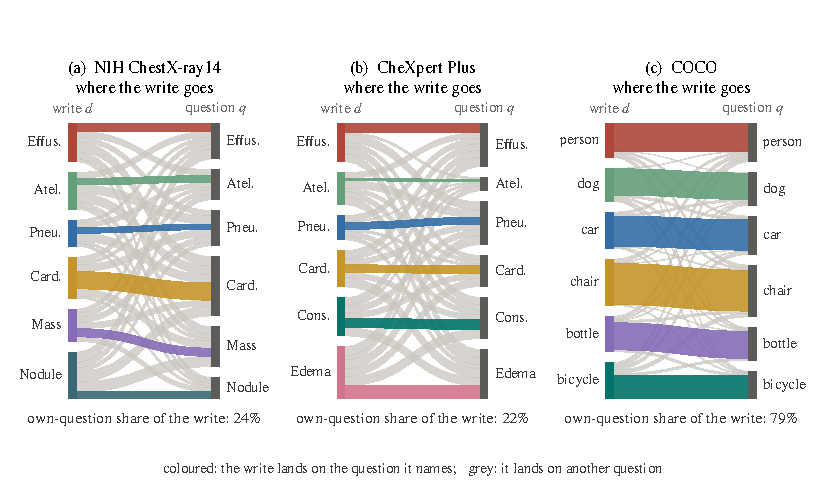
\includegraphics{figures/fig7_write_flow.pdf}}
    \caption{\textbf{Where the write goes.} Bands join each written direction $d$ to the questions $q$ it moves, with width proportional to $F_{q,d}$, the mean over checkpoints of $\max(W_{q,d},0)$. The percentage is the own-question share $\sum_d F_{d,d}/\sum_{q,d} F_{q,d}$.}
    \label{fig:write-flow}
\end{figure}

\begin{figure}[t]
    \centering
    \resizebox{\textwidth}{!}{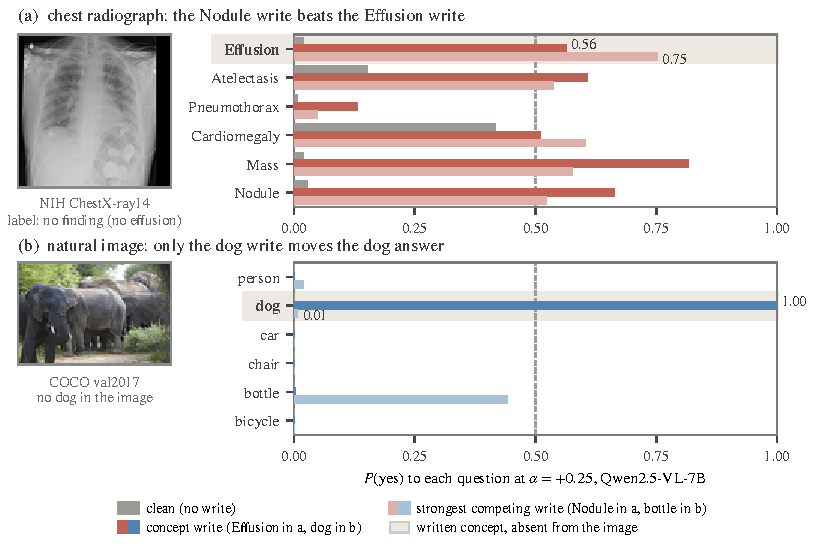
\includegraphics{figures/fig3_example.pdf}}
    \caption{\textbf{Two images, six questions, three writes.} $P(\mathrm{yes})$ per question for an NIH radiograph (top) and a COCO image (bottom), clean and under the concept write and the strongest competing write ($\alpha=+0.25$, Qwen2.5-VL-7B). The shaded row is the written concept, absent from the image; the dashed line marks $P(\mathrm{yes})=0.5$.}
    \label{fig:example}
\end{figure}

\begin{figure}[t]
    \centering
    \resizebox{\textwidth}{!}{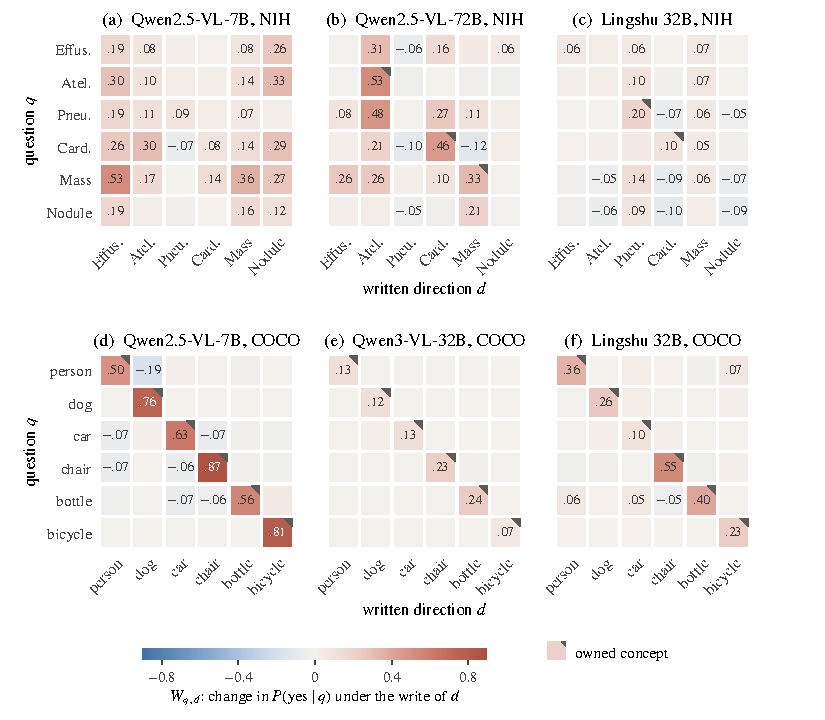
\includegraphics{figures/fig4_write_matrices.pdf}}
    \caption{\textbf{Write matrices.} $W_{q,d}$, the mean change in $P(\mathrm{yes})$ of question $q$ (rows) under the write of direction $d$ (columns), for three checkpoints on NIH (top) and three on COCO (bottom). A corner mark flags owned concepts.}
    \label{fig:write-matrices}
\end{figure}

\subsection{The write mechanism is intact on natural objects}
\label{sec:coco}

On COCO, the same procedure yields the opposite result (Table~\ref{tab:cf-main}, right block). Object ownership holds in \cfCocoOwned{} of \cfCocoOwnedN{} cells (\cfCocoOwnedPct\%), \cfCocoRefMet{} cells meet the steering reference, only \cfCocoCompetitor{} have a stronger competitor, and \cfCocoBlocksFourPlus{} of the \cfCocoBlocks{} checkpoints own at least four of the six objects. Ownership also tracks the dose: on COCO, median ownership rises from $\cfDoseCocoLow$ at $\alpha=-0.1$ to $\cfDoseCocoPeak$ at $\alpha=+0.25$ and stays positive at $\alpha=+0.5$ ($\cfDoseCocoHalf$), while on NIH it stays between $\cfDoseNihMin$ and $\cfDoseNihMax$ at every dose (Figure~\ref{fig:overview}c). The write, direction construction, reference family, and decision rules thus work as intended.

The contrast survives two difficulty controls. Six small or fine-grained COCO categories (handbag, book, backpack, traffic light, knife, and cell phone) remain owned in \cfFgFineOwned{} of \cfFgFineCells{} cells, against \cfFgEasySameOwned{} of \cfFgEasySameCells{} for the easy six in the same \cfFgSameBlocks{} checkpoints (sign test $p=\cfFgSameSignP$), at a median clean-answer AUROC of \cfFgFineAuroc{} against \cfFgEasySameAuroc{}. On the chest sets, ownership also stays rare where the model already answers the question well: at a clean-answer AUROC of at least \cfStratTopEdge{}, \cfStratChestTopOwned{} of \cfStratChestTopN{} chest cells are owned (\cfStratChestTopPct\%) against \cfStratNatTopOwned{} of \cfStratNatTopN{} natural-image cells (\cfStratNatTopPct\%), a difference of $\cfStratCvnDiff$ $[\cfStratCvnLo,\cfStratCvnHi]$ (Appendix~\ref{app:cf-difficulty} states the category rule, the bins, and the bootstrap).

\subsection{The reader decides ownership}
\label{sec:reader}

Checkpoints that share a vision tower differ in what they own. Gemma~3 shares one SigLIP tower across its 4B, 12B, and 27B checkpoints, MedGemma one MedSigLIP tower across 4B and 27B, and LLaVA-1.5 one CLIP tower across 7B and 13B. Within each family, pooled features, fitted probes, and lifted write vectors are identical across sizes (Table~\ref{tab:cf-pairs}), so readability is identical by construction and only the connector and language model that read the written representation differ. Steering a feature of the vision tower and letting the language model say what it sees treats that language model as a stable read-out of the tower \citep{ferrando2026explain}; here the read-out is what varies. In \cfPairsFiveOrSix{} of the \cfPairsN{} shared-tower pair--dataset combinations, the paired patient-bootstrap interval for the between-reader difference $\Delta O_q$ excludes zero for five or six of the six concepts (Figure~\ref{fig:readers}). On NIH Effusion, the identical write on the same 600 patients yields an $O_q$ difference of $\cfPairDeltaEffFourTwelve$ $[\cfPairDeltaEffFourTwelveLo,\cfPairDeltaEffFourTwelveHi]$ between Gemma~3 4B and 12B. In 12B, competing directions win the chest answers outright ($O_{\mathrm{Effusion}}=\cfOGemmaTwelveEff$ on both chest sets), and LLaVA-1.5 7B and 13B own no chest concept yet own \cfLlavaSevenCoco{} and \cfLlavaThirteenCoco{} COCO objects with the same write (Appendix~\ref{app:cf-reader}).

A better chest representation does not supply the missing reader. The three checkpoints whose towers are trained on chest radiographs read and answer the findings best in the grid (median probe AUROC \cfSpecTowerProbeAuroc{} on NIH against \cfSpecRestProbeAuroc{} for the other NIH cells; median clean-answer AUROC \cfSpecTowerAnsAuroc{} against \cfSpecMedAnsAuroc{} and \cfSpecGenAnsAuroc{} for medically tuned and general checkpoints), yet they own \cfSpecTowerOwned{} of their \cfSpecTowerN{} chest cells, against \cfSpecMedOwned{} of \cfSpecMedN{} for medically tuned checkpoints on general towers and \cfSpecGenOwned{} of \cfSpecGenN{} for general checkpoints. Scale raises chest ownership within some families, from none at Qwen2.5-VL 3B and 7B to three NIH concepts at 72B and from three to five CheXpert concepts across Lingshu 7B and 32B, but answering alone does not produce it: InternVL3.5 answers every NIH question at every size while its chest writes stay within $\cfInternvlWqqMax$ of zero (Figure~\ref{fig:ladders}). Ownership is therefore a property of the checkpoint that reads the representation, and a probe fitted to the tower alone cannot certify it.

\begin{figure}[t]
    \centering
    \resizebox{\textwidth}{!}{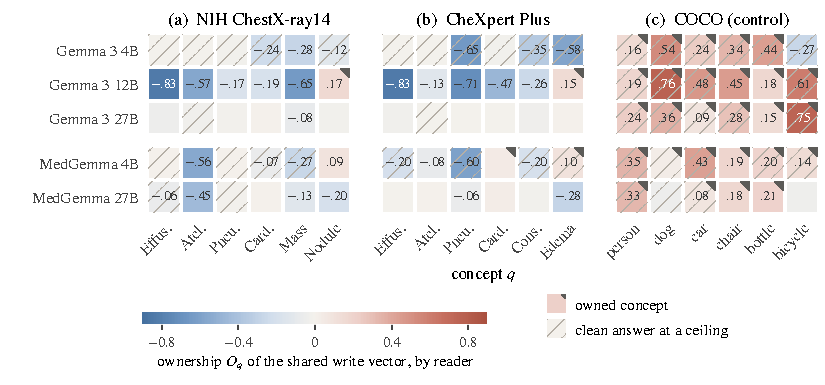
\includegraphics{figures/fig5_same_write.pdf}}
    \caption{\textbf{Same write, different reader.} Ownership $O_q$ per concept on NIH, CheXpert, and COCO for Gemma~3 4B/12B/27B and MedGemma 4B/27B, whose probes and write vectors are identical across sizes within each family. Corner marks flag owned cells and hatching marks ceiling cells.}
    \label{fig:readers}
\end{figure}

\subsection{Non-clinical attributes of the radiograph share the deficit}
\label{sec:attributes}

A non-clinical property of the same film is owned as rarely as a finding. We combine projection, sex, age, and the findings into one nine-direction family. The attribute probes read their labels at least as well as the clinical probes read the findings (median probe AUROC \cfAttrAurocMin{}--\cfAttrAurocMax{} against \cfAttrClinAuroc{}; Table~\ref{tab:cf-attr}), yet attribute cells are owned in \cfAttrAllAttrOwned{} of \cfAttrAllAttrN{} cases and finding cells in \cfAttrAllClinOwned{} of \cfAttrAllClinN{}, the same rate. At a clean-answer AUROC of at least \cfStratTopEdge{}, attributes are owned in \cfStratAttrTopOwned{} of \cfStratAttrTopN{} cells and findings in \cfStratFindTopOwned{} of \cfStratFindTopN{}. The deficit therefore follows the chest-radiograph representation and its reader rather than the concept's clinical status.

\subsection{The direction the reader responds to}
\label{sec:ansdir}

For each question we fit the model's own clean answer margin $\ell_{\mathrm{yes}}-\ell_{\mathrm{no}}$ on training rows from the same projected, train-scaled features by ridge regression, lift the fitted coefficients with Equation~\ref{eq:lift}, and write the result on the test rows exactly as we write a label direction (Table~\ref{tab:cf-ansdir}). This \emph{answer direction} $a_q$ is a handle where the label direction is not. Across the \cfAnsChestN{} chest cells of \cfAnsChestBlocks{} blocks, $a_q$ is owned in \cfAnsChestOwnedA{} and the label direction in \cfAnsChestOwnedLabel{}, and $a_q$ remains owned in \cfAnsdirtChestKept{} of \cfAnsdirtChestKeptN{} chest (cell, template) pairs under the five held-out templates. The features that identify a concept differ from the features that control the output \citep{arad2025saes}; here that separation holds against matched clinical competitors.

The answer direction reads the model, not the label. Over the \cfValAurocAnsChestN{} chest cells, its median AUROC against the report label is $\cfValAurocAnsChest$, against $\cfValAurocProbeChest$ for the probe, while against the model's own clean answer it is $\cfValAurocAnsCleanChest$, against $\cfValAurocProbeCleanChest$ (Table~\ref{tab:cf-validation}). The two directions are far apart on chest radiographs, with a median raw model-space cosine of $\cfAnsCosChestMed$, and substantially aligned on natural images ($\cfAnsCosCocoMed$). The separation persists at four endpoints that fit neither direction (Table~\ref{tab:cf-semend}): the negated question, a forced choice against the strongest competitor in each of its two presentation orders, and the finding word's log-probability in a report continuation. Across the \cfSemCells{} endpoint cells, the answer direction is owned in \cfSemAnswerOwned{} and the label direction in \cfSemLabelOwned{}. On chest radiographs, the direction the model answers along is not the direction the probe fits.

\subsection{Controls and alternatives}
\label{sec:controls}

The reference family behaves as designed: owned concept writes rank 1--6 among the 120 compared effects, and the concept write typically ranks in the top decile on the chest sets (Figure~\ref{fig:overview}d). The deficit survives every alternative we tested; Appendix~\ref{app:cf-ledger} states the reference and rule of each of the \cfLedgerAnalyses{} graded analyses, and Appendix~\ref{app:cf-robustness} gives the details.
\label{sec:robust-geometry}

\paragraph{Geometry, scale, and numerics.} The strongest competitor matches the most similar direction or the most co-occurring label only at chance rate (Table~\ref{tab:cf-geometry}). The logit-scale grade agrees with the probability-scale grade in \cfScaleAgree{} of \cfScaleAgreeN{} cells; restricting each cell to unsaturated rows preserves the owned grade in \cfScaleUnsatGradeKept{} of \cfScaleUnsatGradeN{} owned chest cells; refitting the probes on resampled training patients changes $O_q$ by a median of \cfScaleRefitMedian{}; and rescoring in fp32 at batch size one alters \cfPrecisionGradeChanges{} of \cfPrecisionGradeCells{} grades (Appendix~\ref{app:cf-robustness}).

\paragraph{Labels.} Re-grading the fitted directions on \cfValidRows{} CheXpert films labelled by radiologist consensus \citep{irvin2019chexpert} reproduces the owned grade in \cfValidOwnedAgree{} of \cfValidCells{} cells, and directions refitted on those labels are owned in \cfValidfitOwnedExpert{} of \cfValidfitCells{} cells, against \cfValidfitOwnedReport{} for the report-label directions (Appendix~\ref{app:cf-robustness}).

\paragraph{Directions.} Four alternative constructions, the difference of class means, the Haufe pattern (the training covariance applied to the probe weights; \citealp{haufe2014interpretation}), the normal orthogonalised against the other five normals, and the normal refitted on features residualised against the other five labels \citep{nicolson2025explaining}, are each owned in \cfAltdirChestPctMin{}--\cfAltdirChestPctMax\% of a chest dataset's cells against \cfAltdirCocoPctMin{}--\cfAltdirCocoPctMax\% of COCO cells. Extending the competitor family to every additional dataset label with enough support retains \cfExtcompRetained{} of the \cfExtcompOwned{} owned cells, and writes concentrated on the tokens the probe reads are owned in \cfTokenwSoftChestOwned{} (softmax-weighted) and \cfTokenwTopqChestOwned{} (top quarter) of \cfTokenwChestCells{} chest cells, against \cfTokenwUniformChestOwned{} for the uniform write (Table~\ref{tab:cf-altdir}). Concentrating the write where the probe reads does not create a clinical handle.

\FloatBarrier

\section{Discussion}
\label{sec:implications}

\paragraph{Readability belongs to the probe, ownership to the reader.}
Readability describes a classifier fitted to the representation; ownership describes how the model reading that representation responds to a write. Checkpoints sharing a vision tower have identical probes and write vectors, yet own different concepts, and the chest-trained towers read and answer findings best in the grid but own only \cfSpecTowerOwned{} of \cfSpecTowerN{} chest cells. Ownership therefore belongs on the scorecard of the checkpoint to be deployed rather than on that of the vision tower it contains.

\paragraph{On chest radiographs, the label direction and the answer direction come apart.}
On natural images, the label direction and the model's answer direction are substantially aligned, and writing the label direction controls the answer. On chest radiographs the two are nearly orthogonal: the label direction barely moves its own answer while moving the other findings' answers, and the answer direction is owned in about half of the chest cells. The flat rows of the chest write matrices fit a reader that responds to a signal shared across findings rather than to each finding's own direction \citep{pahde2025navigating}; which signal that is remains open. A legible label need not mark the direction along which the reader chooses its answer, so concept control is a property of a direction and a reader together.

\paragraph{What a steering evaluation should report.}
Probe accuracy and answer accuracy, the two quantities most often reported for medical VLMs, are both high in this grid, yet ownership is \cfChestOwnedPct\%. Random and sham writes show that a direction reaches the answer; only directions fitted the same way for the competing findings, written at the same locus and dose in the same patients, show whether the direction belongs to its label. Studies that use probe normals as interventions should report the write matrix $W$, compare $O_q$ across layers, doses, and models, and pair every clinical write with a natural-image control, where the same procedure produces selective control.


\section{Conclusion}
\label{sec:conclusion}

Reading a clinical concept from a vision-language model's visual representation does not make its probe direction a handle on that concept. Across \cfCheckpoints{} checkpoints and two chest-radiograph datasets, concepts are readable in \cfChestReadablePct\% and answerable in \cfChestAnswerablePct\% of cells but owned in \cfChestOwnedPct\%, because the concept's own direction barely moves its answer while the directions fitted for the other findings move it as much or more. Under the same procedure \cfCocoOwnedPct\% of natural-object cells are owned, also at matched answer ability. Checkpoints that write identical vectors own different concepts, and the model's own answer direction, nearly orthogonal to the probe direction on chest radiographs, provides the handle that the label direction lacks. Readability is a property of a classifier fitted to the representation; control is a property of a direction and the model that reads it.

\section{Limitations}
\label{sec:limitations}

The grades describe linear writes at two loci, the consumed block and the connector output, at one primary dose with a five-point sweep; deeper language-model layers and nonlinear edits may behave differently. Each dataset contributes six concepts, and the chest labels are report-derived, with radiologist labels available for a CheXpert validation subset. The grade needs a discrete answer. MAIRA-2 \citep{bannur2024maira} emits reports rather than answers and fails the image-free mapping check on every template (Appendix~\ref{app:cf-gates}), and the discrete-diffusion report generator of \citet{chen2026echo} has the same shape, so both fall outside the evaluation.

Ownership is a verdict on the write comparison rather than a predictor of effect size. On the four semantic endpoints, adding the ownership contrast to write magnitude, probe selectivity, and clean-answer AUROC adds no held-out predictive value beyond a permutation null ($p=\cfSemCvLocoP$ and $p=\cfSemCvLoboP$ under the concept and block splits; Appendix~\ref{app:cf-ansdir}). The answer direction is fitted on training rows to the model's own clean answers and written on test rows and held-out templates, so it is a handle on the model's answer. Its median AUROC against the report label is $\cfValAurocAnsChest$, below the probe's $\cfValAurocProbeChest$, and answer control and clinical fidelity remain distinct objectives.

\section*{Reproducibility statement}
The registered protocol file fixes the loci, projection, probe settings, dose grid, reference family, templates, modules, gates, and decision rules. The release contains the evaluation code and adapters, the protocol file, the cohort manifests with their seeds, the fitted directions, the per-image outcomes of every module, every block's scorecard and coverage file, the rendered prompts, and the pinned checkpoint revisions (Table~\ref{tab:cf-models}); every table and figure in the paper is regenerated from those files by the scripts in the release. Appendix~\ref{app:repro} states the consumed block of every family, the consumed-token mask, the projection and probe construction, the control sampling procedures, the cohort roles, and the protocol amendments with their dates.

\section*{Ethics statement}
The study uses three public datasets under their published terms: NIH ChestX-ray14 (NIH Clinical Center), CheXpert Plus (Stanford AIMI, accessed through its data-use agreement), and COCO (annotations CC BY 4.0). All radiographs are de-identified by their providers; no protected health information was accessed, and no image or report is redistributed. The write test evaluates model behaviour under activation edits and is not a diagnostic tool; its grades describe what a probe direction does inside a model and carry no claim of clinical benefit.

\bibliography{refs}
\bibliographystyle{plainnat}

\clearpage
\appendix
\section{Campaign details}
\label{app:campaign}

This appendix lists the checkpoints and their consumed loci, the acceptance decisions, the coverage of the campaign, and the per-concept results of every completed block.

\subsection{Labels, registration, and artifact}
\label{app:cf-labels}

\paragraph{Labels.} We use each dataset's supplied report-derived labels: NIH ChestX-ray14 finding labels \citep{wang2017chestxray}, the CheXpert labeler output \citep{irvin2019chexpert} distributed with CheXpert Plus \citep{chambon2024chexpertplus}, and COCO instance annotations \citep{lin2014coco}. Rows are positive for label 1, negative for label 0, and \emph{unknown} when the labeler output is uncertain or blank, which is the uncertainty convention of the CheXpert labeler \citep{irvin2019chexpert}. We exclude unknown rows from probe fitting, selectivity, and answer AUROC. We write and score them like all other rows. Fixed manifests drawn with recorded seeds define the cohorts, one manifest per dataset for every block. No patient and no image appears in two roles of a dataset. Every cohort is disjoint from every pilot-study cohort. Three cohorts are scored: the training cohort for fitting the scaler, probes, and answer direction; the 400-row calibration cohort for the readable and answerable grades; and the 600-row test cohort for every write. A second CheXpert cohort contains \cfValidRows{} frontal films from the CheXpert validation set, one per patient, with the radiologists' consensus labels \citep{irvin2019chexpert}. This cohort has zero patient overlap with any campaign cohort.

\paragraph{Registration.} We froze the protocol before scoring any grid block. The loci, projection and probe settings, dose, reference family, six templates, module set, seven gates, and three decision rules match the registered protocol file. We registered the pilot study's crossover and confirmation analyses before running them (Appendix~\ref{app:seed}). After completing the grid, we added the leaderboard, write-flow share, and per-image examples as descriptive summaries of these outputs.

\paragraph{Artifact.} The release includes evaluation code, adapters, the registered protocol file, cohort manifests with their seeds, and fitted directions. It provides per-image outcomes for every module (write, dose, refit, locus, and template rows), scorecards and coverage files for every block, and rendered prompts. Each new checkpoint requires one adapter that identifies its input block and passes the gates.

\subsection{Grid and consumed loci}
\label{app:cf-grid}

\begin{table}[h]
\centering
\setlength{\tabcolsep}{3pt}
% terracotta = positive / high, blue = negative / low, sage = magnitude of Read and Ans; darker = larger magnitude
\definecolor{cfSage1}{HTML}{ECF3EF}
\definecolor{cfSage2}{HTML}{D5E5DB}
\definecolor{cfSage3}{HTML}{B9D4C3}
\definecolor{cfSage4}{HTML}{9EC3AC}
\definecolor{cfSlate1}{HTML}{EAF0F6}
\definecolor{cfSlate2}{HTML}{D0DDEA}
\definecolor{cfSlate3}{HTML}{B1C7DD}
\definecolor{cfSlate4}{HTML}{94B2D0}
\definecolor{cfTerra1}{HTML}{F7ECEA}
\definecolor{cfTerra2}{HTML}{EED5D1}
\definecolor{cfTerra3}{HTML}{E2B8B2}
\definecolor{cfTerra4}{HTML}{D79E95}
\definecolor{cfOat1}{HTML}{F4EFE6}
\definecolor{cfOat2}{HTML}{E8DDC8}
\definecolor{cfGrey}{HTML}{E4E1DC}

\caption{\textbf{Checkpoints and families.} Per checkpoint: vision tower, consumed tokens per image, input size, and eligible templates. Bold family rows give mean selectivity and clean-answer AUROC over clinical cells and the owned clinical and COCO cells, shaded by owned share.}
\label{tab:cf-models}
\resizebox{\linewidth}{!}{%
\begin{tabular}{lllll@{\hspace{8pt}}rrrr}
\toprule
\multirow{2}{*}{Checkpoint} & \multirow{2}{*}{Vision tower} & \multirow{2}{*}{Tokens} & \multirow{2}{*}{Image} & \multirow{2}{*}{Templates} & \multirow{2}{*}{$\bar S$} & \multirow{2}{*}{$\overline{\mathrm{AUROC}}$} & \multicolumn{2}{c}{owned cells}\\
\cmidrule(lr){8-9}
&  &  &  &  &  &  & \multicolumn{1}{c}{clinical} & \multicolumn{1}{c}{COCO}\\
\midrule
\multicolumn{5}{l}{\textbf{Qwen2.5-VL}~\citep{bai2025qwen25vl}} & 0.132 & 0.635 & \cellcolor{cfTerra2}5/48 & \cellcolor{cfTerra4}24/24 \\
\quad Qwen2.5-VL-3B & native ViT 675M & 576$\to$144 & $336^2$ & IYWYIAWA & & & & \\
\quad Qwen2.5-VL-7B & native ViT 675M & 576$\to$144 & $336^2$ & all & & & & \\
\quad Qwen2.5-VL-32B & native ViT 675M & 576$\to$144 & $336^2$ & all & & & & \\
\quad Qwen2.5-VL-72B & native ViT 675M & 576$\to$144 & $336^2$ & all & & & & \\
\midrule
\multicolumn{5}{l}{\textbf{Qwen3-VL}~\citep{qwen2025qwen3vl}} & 0.137 & 0.735 & \cellcolor{cfTerra2}4/36 & \cellcolor{cfTerra4}18/18 \\
\quad Qwen3-VL-4B & SigLIP2-based & $\leq$1024 & $\leq 512^2$ & all & & & & \\
\quad Qwen3-VL-8B & SigLIP2-based & $\leq$1024 & $\leq 512^2$ & all & & & & \\
\quad Qwen3-VL-32B & SigLIP2-based & $\leq$1024 & $\leq 512^2$ & all & & & & \\
\midrule
\multicolumn{5}{l}{\textbf{InternVL3.5}~\citep{wang2025internvl35}} & 0.125 & 0.807 & \cellcolor{cfTerra2}5/36 & \cellcolor{cfTerra4}17/18 \\
\quad InternVL3.5-8B & InternViT-300M & 1024 & $448^2$ & all & & & & \\
\quad InternVL3.5-14B & InternViT-300M & 1024 & $448^2$ & all & & & & \\
\quad InternVL3.5-38B & InternViT-6B & 1024 & $448^2$ & all & & & & \\
\midrule
\multicolumn{5}{l}{\textbf{Gemma 3}~\citep{gemma2025gemma3}} & 0.124 & 0.564 & \cellcolor{cfTerra2}2/36 & \cellcolor{cfTerra4}17/18 \\
\quad Gemma 3 4B & SigLIP-So400m & 4096 & $896^2$ & all & & & & \\
\quad Gemma 3 12B & SigLIP-So400m & 4096 & $896^2$ & all & & & & \\
\quad Gemma 3 27B & SigLIP-So400m & 4096 & $896^2$ & all & & & & \\
\midrule
\multicolumn{5}{l}{\textbf{MedGemma} (medical)~\citep{sellergren2025medgemma}} & 0.164 & 0.835 & \cellcolor{cfTerra2}2/24 & \cellcolor{cfTerra3}10/12 \\
\quad MedGemma 4B & MedSigLIP & 4096 & $896^2$ & all & & & & \\
\quad MedGemma 27B & MedSigLIP & 4096 & $896^2$ & all & & & & \\
\midrule
\multicolumn{5}{l}{\textbf{Lingshu} (medical)~\citep{lasa2025lingshu}} & 0.142 & 0.820 & \cellcolor{cfTerra4}11/24 & \cellcolor{cfTerra4}12/12 \\
\quad Lingshu 7B & Qwen2.5-VL ViT & 576$\to$144 & $336^2$ & all & & & & \\
\quad Lingshu 32B & Qwen2.5-VL ViT & 576$\to$144 & $336^2$ & all & & & & \\
\midrule
\multicolumn{5}{l}{\textbf{LLaVA-1.5}~\citep{liu2024improved}} & 0.124 & 0.516 & \cellcolor{cfTerra1}0/24 & \cellcolor{cfTerra3}7/12 \\
\quad LLaVA-1.5-7B & CLIP ViT-L/14-336 & 576 & $336^2$ & IYWY & & & & \\
\quad LLaVA-1.5-13B & CLIP ViT-L/14-336 & 576 & $336^2$ & IYWYIAWA & & & & \\
\midrule
\multicolumn{5}{l}{\textbf{LLaVA-Med} (medical)~\citep{li2023llavamed}} & 0.136 & 0.560 & \cellcolor{cfTerra2}1/12 & \cellcolor{cfTerra2}1/6 \\
\quad LLaVA-Med 1.5 7B & CLIP ViT-L/14-336 & 576 & $336^2$ & IYWY & & & & \\
\midrule
\multicolumn{5}{l}{\textbf{Llama 3.2 Vision}~\citep{meta2024llama32vision}} & 0.119 & 0.688 & \cellcolor{cfTerra1}0/12 & \cellcolor{cfTerra2}1/6 \\
\quad Llama 3.2 Vision 11B & ViT-H/14 & 1601 & $560^2$ & IBWB & & & & \\
\midrule
\multicolumn{5}{l}{\textbf{CheXagent} (medical)~\citep{chen2024chexagent}} & 0.180 & 0.857 & \cellcolor{cfTerra3}7/24 & \cellcolor{cfTerra2}2/12 \\
\quad CheXagent-2-3B & XraySigLIP ViT-L/16 & 1024 & $512^2$ & IYWYIAWA & & & & \\
\quad CheXagent-8B & EVA-CLIP ViT 1.4B & 1025$\to$128 & $448^2$ & IYWYIAWA & & & & \\
\midrule
\multicolumn{5}{l}{\textbf{LLaVA-Rad} (medical)~\citep{zambranochaves2025llavarad}} & 0.209 & 0.793 & \cellcolor{cfTerra1}0/12 & \cellcolor{cfTerra1}0/6 \\
\quad LLaVA-Rad-7B & BiomedCLIP-CXR-518 & 1369 & $518^2$ & IYWY & & & & \\
\midrule
\multicolumn{5}{l}{\textbf{HuatuoGPT-Vision} (medical)~\citep{chen2024huatuogptvision}} & 0.136 & 0.746 & \cellcolor{cfTerra2}1/12 & \cellcolor{cfTerra3}4/6 \\
\quad HuatuoGPT-Vision-7B & CLIP ViT-L/14-336 & 576 & $336^2$ & all & & & & \\
\bottomrule
\end{tabular}}
\end{table}

\begin{figure}[h]
    \centering
    \resizebox{\textwidth}{!}{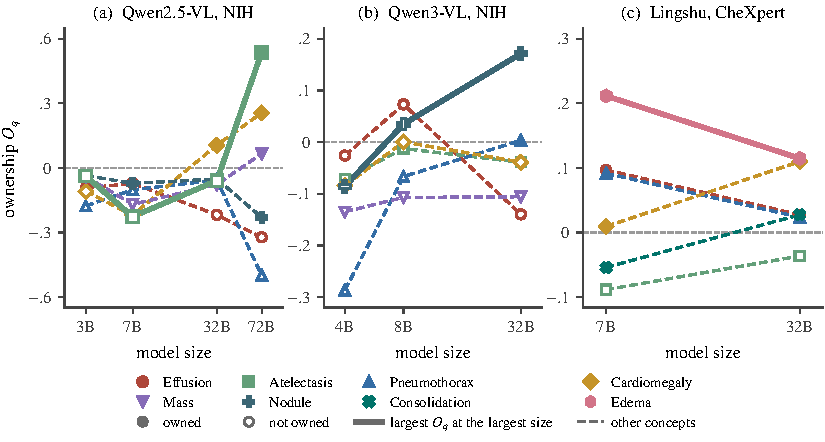
\includegraphics{figures/fig6_ladders.pdf}}
    \caption{\textbf{Size ladders.} Ownership $O_q$ per concept across sizes for Qwen2.5-VL and Qwen3-VL on NIH and Lingshu on CheXpert. Solid lines mark the concept with the largest ownership at the largest size (Atelectasis, Nodule, Edema), filled markers owned cells; vertical scales differ by panel.}
    \label{fig:ladders}
\end{figure}


The towers include CLIP \citep{radford2021clip} in the LLaVA families, SigLIP \citep{zhai2023siglip} in Gemma~3, and a SigLIP~2 design \citep{tschannen2025siglip2} in Qwen3-VL; MedGemma's MedSigLIP tower is a medically tuned SigLIP released with that model \citep{sellergren2025medgemma}. The three towers trained on chest radiographs are the XraySigLIP tower of CheXagent-2-3B \citep{chen2024chexagent}, the EVA-CLIP tower \citep{sun2023evaclip} of CheXagent-8B, and the BiomedCLIP-CXR tower of LLaVA-Rad-7B \citep{zhang2025biomedclip,zambranochaves2025llavarad}; HuatuoGPT-Vision-7B tunes on medical data over the same stock CLIP tower as LLaVA-1.5. Consumed-token counts range from \cfTokensMin{} to \cfTokensMax{} per image, and each family uses a fixed image resolution. The Llama~3.2 Vision projector also reads five intermediate local-layer outputs that bypass the final global block. LLaVA computes the final CLIP block but consumes the penultimate block. At every checkpoint, Gate (C) verifies that the write reaches the consumer and the answer logits and changes nothing outside the consumed tokens.

\subsection{Acceptance decisions}
\label{app:cf-gates}

Seven checks run on the 16 preflight rows at both loci before a block is scored: (A) bitwise determinism; (B) identity at $\alpha=0$; (C) reach, under which the write must change the consumer's input and answer logits without changing anything outside the consumed tokens; (D) batched-versus-single agreement of the answer logits within $0.25$; (E) image-free semantic mapping of every template; (F) throughput; and (G) fp32 recomputation of the answer logits. Deviations in (D) are declared and neutralised by scoring every condition of a question in one fixed batch composition. Templates that fail (E) are ineligible; a checkpoint whose yes/no template fails is graded on its eligible B-positive template (IB for Llama~3.2 Vision), and its scorecards record the template used and every declared deviation.

All \cfWriteBlocks{} completed blocks pass checks (A), (B), (C), and (G): determinism error is zero, change at $\alpha=0$ is zero, and fp32-versus-model logit differences are below \cfGateFpMax{}. In check (D), the Qwen3-VL, Gemma~3, MedGemma, InternVL, and Llama families exceed the 0.25-logit tolerance (up to \cfGateBatchMax{} logits for Gemma~3 12B). We record these as declared deviations. Fixed batch composition neutralises them. Check (E) fails across all datasets for the A/B templates for LLaVA-1.5-7B and LLaVA-Med, the B-mapped templates for Qwen2.5-VL-3B and LLaVA-1.5-13B, and the yes/no and A-mapped templates for Llama~3.2 Vision 11B. We record affected cells as ineligible. Check (E) fails for every template of MAIRA-2 \citep{bannur2024maira} on NIH: the model answers ``No'' to every finding on all \cfSpecUngradedRows{} preflight images and ``A'' to every forced choice under both letter mappings, so no template carries a graded answer and the block produces no outcomes. Two Gemma~3 checkpoints answer ``yes'' to most chest questions; Gemma~3 4B does so on \cfGemmaFourYesMin--\cfGemmaFourYesMax\% of rows (clean $P(\mathrm{yes})>0.99$). The answerability grade records this behaviour. Three checkpoints (LLaVA-1.5 7B/13B, LLaVA-Med) answer at chance.

\subsection{Coverage and cost}
\label{app:cf-coverage}

Every checkpoint has a completed core write matrix and calibration pass on NIH ChestX-ray14, CheXpert Plus, and COCO. The campaign targets \cfCoveragePlannedWord{} modules per block: the write matrix, the calibration pass, the five additional templates, the dose sweep, the two probe refits, the connector locus, and the connector-locus calibration. \cfCoverageBlocksAllSeven{} of \cfBlocks{} blocks carry all seven modules. A probe-graded block whose write matrix is ineligible or incomplete contributes readability alone. Each block's scorecard also reports the dose range of $O_q$ over $\alpha\in[-0.5,0.5]$, its standard deviation over the three fit seeds, ownership at the connector locus, and the wording and mapping contrasts of $O_q$ across the six templates. The partial block is Qwen2.5-VL-72B on CheXpert Plus, which lacks the additional templates and the connector locus. The campaign used about 3,000 A100-hours; a chest block of a 7B checkpoint takes about ten.


\subsection{Ownership of every concept}
\label{app:cf-tables}

Tables~\ref{tab:cf-own-nih}--\ref{tab:cf-own-coco} report the ownership contrast $O_q$ of every concept cell, one table per dataset, with the checkpoints in the order of Table~\ref{tab:cf-main}. Their cells are shaded by magnitude at $0.02$, $0.10$, and $0.25$, terracotta for positive and blue for negative ownership.

\paragraph{NIH ChestX-ray14.} \cfNihOwned{} of the \cfNihCells{} cells are owned, a stronger competitor is identified in \cfNihCompetitor{}, and the contrast is positive in \cfGeoOwnWinsNihPct\% of cells. The owned cells concentrate in a few rows: Qwen2.5-VL-72B owns Atelectasis ($O_q=\cfOQwenSeventyTwoAtel$), Cardiomegaly, and Mass, while in Gemma~3 12B the competing directions win most answers, down to $O_{\mathrm{Effusion}}=\cfOGemmaTwelveEff$.

\begin{table}[htbp]
\centering
\setlength{\tabcolsep}{4pt}
\caption{\textbf{Ownership of every concept, NIH ChestX-ray14.} $O_q$ at $\alpha=+0.25$: bold is owned, $\dagger$ a stronger competitor, $\ddagger$ unresolved; the last row counts owned cells. Shading darkens with $|O_q|$ (terracotta positive, blue negative).}
\label{tab:cf-own-nih}
\resizebox{\linewidth}{!}{%
\begin{tabular}{lrrrrrr}
\toprule
Checkpoint & \multicolumn{1}{c}{Effusion} & \multicolumn{1}{c}{Atelectasis} & \multicolumn{1}{c}{Pneumothorax} & \multicolumn{1}{c}{Cardiomegaly} & \multicolumn{1}{c}{Mass} & \multicolumn{1}{c}{Nodule}\\
\midrule
Lingshu 32B & \cellcolor{cfSlate1}-0.01 & \cellcolor{cfSlate2}-0.08 & \cellcolor{cfTerra3}\textbf{+0.14} & \cellcolor{cfTerra2}\textbf{+0.05} & \cellcolor{cfSlate2}-0.08 & \cellcolor{cfSlate3}-0.18 \\
CheXagent-2-3B & \cellcolor{cfSlate1}-0.00$^{\ddagger}$ & \cellcolor{cfTerra2}\textbf{+0.04} & \cellcolor{cfSlate1}-0.00$^{\dagger}$ & \cellcolor{cfSlate1}-0.01 & \cellcolor{cfTerra1}\textbf{+0.01} & \cellcolor{cfSlate1}-0.01 \\
Qwen2.5-VL-72B & \cellcolor{cfSlate4}-0.32 & \cellcolor{cfTerra4}\textbf{+0.54} & \cellcolor{cfSlate4}-0.50 & \cellcolor{cfTerra4}\textbf{+0.26} & \cellcolor{cfTerra2}\textbf{+0.07} & \cellcolor{cfSlate3}-0.23 \\
Lingshu 7B & \cellcolor{cfTerra1}+0.02 & \cellcolor{cfTerra1}+0.01 & \cellcolor{cfTerra1}+0.01 & \cellcolor{cfTerra3}\textbf{+0.17} & \cellcolor{cfSlate2}-0.09 & \cellcolor{cfTerra1}+0.02 \\
Qwen3-VL-4B & \cellcolor{cfSlate2}-0.03$^{\dagger}$ & \cellcolor{cfSlate2}-0.07 & \cellcolor{cfSlate4}-0.29 & \cellcolor{cfSlate2}-0.08 & \cellcolor{cfSlate3}-0.13 & \cellcolor{cfSlate2}-0.09 \\
Qwen3-VL-32B & \cellcolor{cfSlate3}-0.14 & \cellcolor{cfSlate2}-0.04 & \cellcolor{cfTerra1}+0.00$^{\ddagger}$ & \cellcolor{cfSlate2}-0.04 & \cellcolor{cfSlate3}-0.11 & \cellcolor{cfTerra3}\textbf{+0.17} \\
InternVL3.5-38B & \cellcolor{cfTerra1}+0.00$^{\ddagger}$ & \cellcolor{cfSlate1}-0.02 & \cellcolor{cfSlate1}-0.00 & \cellcolor{cfSlate2}-0.03 & \cellcolor{cfTerra1}+0.02 & \cellcolor{cfTerra1}+0.00 \\
Gemma 3 12B & \cellcolor{cfSlate4}-0.83 & \cellcolor{cfSlate4}-0.57 & \cellcolor{cfSlate3}-0.17 & \cellcolor{cfSlate3}-0.19 & \cellcolor{cfSlate4}-0.65 & \cellcolor{cfTerra3}\textbf{+0.17} \\
MedGemma 4B & \cellcolor{cfTerra1}+0.01 & \cellcolor{cfSlate4}-0.56 & \cellcolor{cfTerra1}+0.01 & \cellcolor{cfSlate2}-0.07 & \cellcolor{cfSlate4}-0.27 & \cellcolor{cfTerra2}+0.09 \\
InternVL3.5-14B & \cellcolor{cfTerra1}\textbf{+0.01} & \cellcolor{cfSlate1}-0.01 & \cellcolor{cfSlate1}-0.00 & \cellcolor{cfSlate1}-0.00 & \cellcolor{cfTerra1}+0.00 & \cellcolor{cfSlate1}-0.01 \\
Qwen2.5-VL-32B & \cellcolor{cfSlate3}-0.22 & \cellcolor{cfSlate2}-0.06 & \cellcolor{cfSlate2}-0.06 & \cellcolor{cfTerra3}\textbf{+0.11} & \cellcolor{cfSlate2}-0.08 & \cellcolor{cfSlate2}-0.05 \\
InternVL3.5-8B & \cellcolor{cfTerra1}+0.00 & \cellcolor{cfSlate1}-0.02 & \cellcolor{cfSlate1}-0.00 & \cellcolor{cfTerra1}+0.00 & \cellcolor{cfSlate1}-0.01 & \cellcolor{cfSlate1}-0.01 \\
HuatuoGPT-Vision-7B & \cellcolor{cfSlate2}-0.04 & \cellcolor{cfSlate2}-0.03 & \cellcolor{cfSlate2}-0.03 & \cellcolor{cfSlate2}-0.08 & \cellcolor{cfSlate2}-0.04 & \cellcolor{cfTerra1}\textbf{+0.01} \\
LLaVA-Med 1.5 7B & \cellcolor{cfSlate1}-0.00 & \cellcolor{cfSlate1}-0.00 & \cellcolor{cfSlate2}-0.04 & \cellcolor{cfSlate1}-0.01 & \cellcolor{cfSlate1}-0.01 & \cellcolor{cfSlate2}-0.02 \\
CheXagent-8B & \cellcolor{cfTerra1}+0.01 & \cellcolor{cfSlate1}-0.01 & \cellcolor{cfSlate1}-0.00 & \cellcolor{cfSlate1}-0.00 & \cellcolor{cfTerra1}+0.00 & \cellcolor{cfSlate1}-0.01 \\
Qwen2.5-VL-3B & \cellcolor{cfSlate2}-0.09 & \cellcolor{cfSlate2}-0.04 & \cellcolor{cfSlate3}-0.18 & \cellcolor{cfSlate3}-0.11 & \cellcolor{cfSlate2}-0.04 & \cellcolor{cfSlate2}-0.04 \\
Qwen2.5-VL-7B & \cellcolor{cfSlate2}-0.07$^{\dagger}$ & \cellcolor{cfSlate3}-0.23 & \cellcolor{cfSlate3}-0.10 & \cellcolor{cfSlate3}-0.22 & \cellcolor{cfSlate3}-0.17 & \cellcolor{cfSlate2}-0.07 \\
Qwen3-VL-8B & \cellcolor{cfTerra2}+0.07 & \cellcolor{cfSlate1}-0.01 & \cellcolor{cfSlate2}-0.07 & \cellcolor{cfTerra1}+0.00 & \cellcolor{cfSlate3}-0.11 & \cellcolor{cfTerra2}+0.03 \\
Gemma 3 27B & \cellcolor{cfSlate2}-0.04 & \cellcolor{cfSlate2}-0.03 & \cellcolor{cfSlate1}-0.01 & \cellcolor{cfTerra1}+0.00$^{\ddagger}$ & \cellcolor{cfSlate2}-0.08 & \cellcolor{cfSlate1}-0.02 \\
Gemma 3 4B & \cellcolor{cfSlate1}-0.00 & \cellcolor{cfSlate1}-0.00 & \cellcolor{cfSlate1}-0.01 & \cellcolor{cfSlate3}-0.24 & \cellcolor{cfSlate4}-0.28 & \cellcolor{cfSlate3}-0.12 \\
LLaVA-1.5-7B & \cellcolor{cfSlate2}-0.03 & \cellcolor{cfSlate1}-0.01 & \cellcolor{cfSlate2}-0.08 & \cellcolor{cfSlate3}-0.13 & \cellcolor{cfTerra2}+0.02 & \cellcolor{cfSlate1}-0.02 \\
MedGemma 27B & \cellcolor{cfSlate2}-0.06 & \cellcolor{cfSlate4}-0.45 & \cellcolor{cfSlate1}-0.01 & \cellcolor{cfTerra1}+0.00 & \cellcolor{cfSlate3}-0.13 & \cellcolor{cfSlate3}-0.20 \\
LLaVA-1.5-13B & \cellcolor{cfSlate1}-0.01 & \cellcolor{cfSlate2}-0.05 & \cellcolor{cfSlate2}-0.04 & \cellcolor{cfSlate2}-0.03 & \cellcolor{cfTerra1}+0.01 & \cellcolor{cfSlate1}-0.02 \\
Llama 3.2 Vision 11B & \cellcolor{cfSlate2}-0.04 & \cellcolor{cfSlate2}-0.07 & \cellcolor{cfSlate2}-0.05 & \cellcolor{cfTerra2}+0.02 & \cellcolor{cfSlate2}-0.06 & \cellcolor{cfSlate1}-0.01 \\
LLaVA-Rad-7B & \cellcolor{cfSlate1}-0.02 & \cellcolor{cfSlate1}-0.01 & \cellcolor{cfSlate1}-0.00 & \cellcolor{cfTerra1}+0.00 & \cellcolor{cfSlate1}-0.01 & \cellcolor{cfSlate2}-0.03 \\
\midrule
\textbf{Owned} & 1 & 2 & 1 & 4 & 2 & 3 \\
\bottomrule
\end{tabular}}
\end{table}

\paragraph{CheXpert Plus.} \cfChexOwned{} of the \cfChexCells{} cells are owned, \cfChexCompetitor{} have a stronger competitor, and the contrast is positive in \cfGeoOwnWinsChexPct\% of cells. Lingshu contributes the largest share of the owned cells, with three concepts at 7B and five at 32B.

\begin{table}[htbp]
\centering
\setlength{\tabcolsep}{4pt}
\caption{\textbf{Ownership of every concept, CheXpert Plus.} As Table~\ref{tab:cf-own-nih}.}
\label{tab:cf-own-chexpert}
\resizebox{\linewidth}{!}{%
\begin{tabular}{lrrrrrr}
\toprule
Checkpoint & \multicolumn{1}{c}{Effusion} & \multicolumn{1}{c}{Atelectasis} & \multicolumn{1}{c}{Pneumothorax} & \multicolumn{1}{c}{Cardiomegaly} & \multicolumn{1}{c}{Consolidation} & \multicolumn{1}{c}{Edema}\\
\midrule
Lingshu 32B & \cellcolor{cfTerra2}\textbf{+0.03} & \cellcolor{cfSlate2}-0.04$^{\dagger}$ & \cellcolor{cfTerra2}\textbf{+0.02} & \cellcolor{cfTerra3}\textbf{+0.11} & \cellcolor{cfTerra2}\textbf{+0.03} & \cellcolor{cfTerra3}\textbf{+0.11} \\
CheXagent-2-3B & \cellcolor{cfTerra2}\textbf{+0.03} & \cellcolor{cfSlate2}-0.02 & \cellcolor{cfTerra1}\textbf{+0.01} & \cellcolor{cfTerra1}\textbf{+0.02} & \cellcolor{cfTerra1}\textbf{+0.01} & \cellcolor{cfSlate1}-0.00$^{\ddagger}$ \\
Qwen2.5-VL-72B & \cellcolor{cfSlate3}-0.12 & \cellcolor{cfTerra2}+0.09 & \cellcolor{cfTerra2}\textbf{+0.03} & \cellcolor{cfSlate3}-0.11 & \cellcolor{cfSlate4}-0.29 & \cellcolor{cfSlate3}-0.13 \\
Lingshu 7B & \cellcolor{cfTerra2}\textbf{+0.10} & \cellcolor{cfSlate2}-0.09 & \cellcolor{cfTerra2}\textbf{+0.09} & \cellcolor{cfTerra1}+0.01$^{\ddagger}$ & \cellcolor{cfSlate2}-0.05 & \cellcolor{cfTerra3}\textbf{+0.21} \\
Qwen3-VL-4B & \cellcolor{cfSlate1}-0.01$^{\dagger}$ & \cellcolor{cfSlate1}-0.02 & \cellcolor{cfSlate3}-0.23 & \cellcolor{cfSlate1}-0.01 & \cellcolor{cfTerra2}\textbf{+0.09} & \cellcolor{cfTerra2}\textbf{+0.09} \\
Qwen3-VL-32B & \cellcolor{cfSlate2}-0.04 & \cellcolor{cfTerra1}+0.00$^{\ddagger}$ & \cellcolor{cfTerra1}+0.00 & \cellcolor{cfSlate2}-0.03 & \cellcolor{cfSlate3}-0.12 & \cellcolor{cfTerra2}\textbf{+0.05} \\
InternVL3.5-38B & \cellcolor{cfTerra1}\textbf{+0.02} & \cellcolor{cfSlate1}-0.01 & \cellcolor{cfSlate1}-0.00 & \cellcolor{cfSlate1}-0.00$^{\ddagger}$ & \cellcolor{cfTerra1}\textbf{+0.01} & \cellcolor{cfSlate2}-0.02 \\
Gemma 3 12B & \cellcolor{cfSlate4}-0.83 & \cellcolor{cfSlate3}-0.13 & \cellcolor{cfSlate4}-0.71 & \cellcolor{cfSlate4}-0.47 & \cellcolor{cfSlate4}-0.26 & \cellcolor{cfTerra3}\textbf{+0.15} \\
MedGemma 4B & \cellcolor{cfSlate3}-0.20 & \cellcolor{cfSlate2}-0.08 & \cellcolor{cfSlate4}-0.60 & \cellcolor{cfTerra2}\textbf{+0.04} & \cellcolor{cfSlate3}-0.20 & \cellcolor{cfTerra3}\textbf{+0.10} \\
InternVL3.5-14B & \cellcolor{cfTerra1}\textbf{+0.01} & \cellcolor{cfSlate1}-0.00 & \cellcolor{cfTerra1}+0.00 & \cellcolor{cfSlate1}-0.01 & \cellcolor{cfTerra1}+0.01 & \cellcolor{cfSlate1}-0.00 \\
Qwen2.5-VL-32B & \cellcolor{cfSlate2}-0.07 & \cellcolor{cfSlate3}-0.19 & \cellcolor{cfSlate3}-0.12 & \cellcolor{cfSlate3}-0.19 & \cellcolor{cfSlate2}-0.05 & \cellcolor{cfSlate2}-0.02 \\
InternVL3.5-8B & \cellcolor{cfSlate1}-0.01 & \cellcolor{cfSlate1}-0.01 & \cellcolor{cfTerra1}\textbf{+0.00} & \cellcolor{cfSlate1}-0.00 & \cellcolor{cfTerra1}+0.01 & \cellcolor{cfSlate1}-0.00 \\
HuatuoGPT-Vision-7B & \cellcolor{cfSlate2}-0.02 & \cellcolor{cfSlate1}-0.02 & \cellcolor{cfSlate1}-0.00 & \cellcolor{cfTerra1}+0.01 & \cellcolor{cfSlate2}-0.03 & \cellcolor{cfSlate1}-0.01 \\
LLaVA-Med 1.5 7B & \cellcolor{cfTerra1}\textbf{+0.00} & \cellcolor{cfSlate1}-0.00 & \cellcolor{cfSlate2}-0.02 & \cellcolor{cfSlate2}-0.03 & \cellcolor{cfSlate1}-0.00$^{\dagger}$ & \cellcolor{cfSlate1}-0.02 \\
CheXagent-8B & \cellcolor{cfSlate2}-0.02 & \cellcolor{cfSlate1}-0.02 & \cellcolor{cfSlate2}-0.02 & \cellcolor{cfSlate2}-0.07 & \cellcolor{cfTerra2}\textbf{+0.04} & \cellcolor{cfSlate2}-0.02 \\
Qwen2.5-VL-3B & \cellcolor{cfSlate3}-0.18 & \cellcolor{cfSlate1}-0.02 & \cellcolor{cfSlate2}-0.04 & \cellcolor{cfSlate2}-0.05 & \cellcolor{cfSlate2}-0.03 & \cellcolor{cfSlate2}-0.08 \\
Qwen2.5-VL-7B & \cellcolor{cfTerra1}+0.01 & \cellcolor{cfSlate2}-0.05 & \cellcolor{cfSlate2}-0.10 & \cellcolor{cfSlate1}-0.00 & \cellcolor{cfSlate3}-0.15 & \cellcolor{cfSlate3}-0.18 \\
Qwen3-VL-8B & \cellcolor{cfSlate2}-0.07$^{\dagger}$ & \cellcolor{cfSlate1}-0.00$^{\dagger}$ & \cellcolor{cfSlate2}-0.10 & \cellcolor{cfSlate1}-0.00 & \cellcolor{cfSlate2}-0.04$^{\dagger}$ & \cellcolor{cfSlate2}-0.06 \\
Gemma 3 27B & \cellcolor{cfSlate2}-0.03 & \cellcolor{cfSlate1}-0.00 & \cellcolor{cfSlate1}-0.01 & \cellcolor{cfSlate1}-0.00 & \cellcolor{cfSlate2}-0.03 & \cellcolor{cfTerra1}+0.00$^{\ddagger}$ \\
Gemma 3 4B & \cellcolor{cfSlate1}-0.00 & \cellcolor{cfSlate1}-0.00 & \cellcolor{cfSlate4}-0.65 & \cellcolor{cfSlate1}-0.02 & \cellcolor{cfSlate4}-0.35 & \cellcolor{cfSlate4}-0.58 \\
LLaVA-1.5-7B & \cellcolor{cfTerra1}+0.00 & \cellcolor{cfSlate2}-0.09 & \cellcolor{cfSlate2}-0.10 & \cellcolor{cfTerra2}+0.03 & \cellcolor{cfSlate2}-0.03 & \cellcolor{cfSlate1}-0.00 \\
MedGemma 27B & \cellcolor{cfSlate1}-0.01 & \cellcolor{cfTerra1}+0.00 & \cellcolor{cfSlate2}-0.06 & \cellcolor{cfTerra2}+0.03 & \cellcolor{cfSlate1}-0.02 & \cellcolor{cfSlate4}-0.28 \\
LLaVA-1.5-13B & \cellcolor{cfSlate1}-0.00 & \cellcolor{cfSlate2}-0.03 & \cellcolor{cfSlate1}-0.01 & \cellcolor{cfTerra1}+0.00 & \cellcolor{cfTerra1}+0.01 & \cellcolor{cfSlate1}-0.01 \\
Llama 3.2 Vision 11B & \cellcolor{cfSlate1}-0.01 & \cellcolor{cfSlate2}-0.05 & \cellcolor{cfSlate2}-0.08 & \cellcolor{cfSlate2}-0.07 & \cellcolor{cfSlate2}-0.05 & \cellcolor{cfSlate1}-0.01 \\
LLaVA-Rad-7B & \cellcolor{cfSlate2}-0.04 & \cellcolor{cfSlate1}-0.01 & \cellcolor{cfTerra1}+0.00 & \cellcolor{cfSlate2}-0.07 & \cellcolor{cfTerra2}+0.02 & \cellcolor{cfSlate1}-0.00 \\
\midrule
\textbf{Owned} & 6 & 0 & 5 & 3 & 5 & 6 \\
\bottomrule
\end{tabular}}
\end{table}

\paragraph{COCO.} \cfCocoOwned{} of the \cfCocoOwnedN{} cells are owned and \cfCocoCompetitor{} have a stronger competitor, and \cfCocoBlocksFourPlus{} of the \cfCocoBlocks{} checkpoints own at least four of the six objects. The rows without owned objects are CheXagent-8B and LLaVA-Rad-7B, whose clean answers to the COCO questions are near chance (Table~\ref{tab:cf-main}).

\begin{table}[htbp]
\centering
\setlength{\tabcolsep}{11pt}
\caption{\textbf{Ownership of every concept, COCO.} As Table~\ref{tab:cf-own-nih}.}
\label{tab:cf-own-coco}
\resizebox{\linewidth}{!}{%
\begin{tabular}{lrrrrrr}
\toprule
Checkpoint & \multicolumn{1}{c}{person} & \multicolumn{1}{c}{dog} & \multicolumn{1}{c}{car} & \multicolumn{1}{c}{chair} & \multicolumn{1}{c}{bottle} & \multicolumn{1}{c}{bicycle}\\
\midrule
Lingshu 32B & \cellcolor{cfTerra4}\textbf{+0.29} & \cellcolor{cfTerra3}\textbf{+0.23} & \cellcolor{cfTerra2}\textbf{+0.08} & \cellcolor{cfTerra4}\textbf{+0.53} & \cellcolor{cfTerra4}\textbf{+0.34} & \cellcolor{cfTerra3}\textbf{+0.22} \\
CheXagent-2-3B & \cellcolor{cfTerra2}\textbf{+0.07} & \cellcolor{cfTerra2}\textbf{+0.07} & \cellcolor{cfTerra2}+0.03 & \cellcolor{cfSlate1}-0.01 & \cellcolor{cfTerra2}+0.04 & \cellcolor{cfTerra1}+0.00 \\
Qwen2.5-VL-72B & \cellcolor{cfTerra4}\textbf{+0.66} & \cellcolor{cfTerra4}\textbf{+0.44} & \cellcolor{cfTerra4}\textbf{+0.95} & \cellcolor{cfTerra4}\textbf{+0.89} & \cellcolor{cfTerra4}\textbf{+0.62} & \cellcolor{cfTerra4}\textbf{+0.40} \\
Lingshu 7B & \cellcolor{cfTerra4}\textbf{+0.39} & \cellcolor{cfTerra4}\textbf{+0.74} & \cellcolor{cfTerra4}\textbf{+0.70} & \cellcolor{cfTerra4}\textbf{+0.76} & \cellcolor{cfTerra4}\textbf{+0.64} & \cellcolor{cfTerra4}\textbf{+0.85} \\
Qwen3-VL-4B & \cellcolor{cfTerra4}\textbf{+0.46} & \cellcolor{cfTerra3}\textbf{+0.13} & \cellcolor{cfTerra4}\textbf{+0.33} & \cellcolor{cfTerra4}\textbf{+0.71} & \cellcolor{cfTerra4}\textbf{+0.34} & \cellcolor{cfTerra2}\textbf{+0.07} \\
Qwen3-VL-32B & \cellcolor{cfTerra3}\textbf{+0.13} & \cellcolor{cfTerra3}\textbf{+0.12} & \cellcolor{cfTerra3}\textbf{+0.11} & \cellcolor{cfTerra3}\textbf{+0.23} & \cellcolor{cfTerra3}\textbf{+0.24} & \cellcolor{cfTerra2}\textbf{+0.07} \\
InternVL3.5-38B & \cellcolor{cfTerra1}\textbf{+0.01} & \cellcolor{cfTerra1}\textbf{+0.00} & \cellcolor{cfTerra1}\textbf{+0.01} & \cellcolor{cfTerra1}\textbf{+0.02} & \cellcolor{cfTerra1}\textbf{+0.01} & \cellcolor{cfTerra1}\textbf{+0.01} \\
Gemma 3 12B & \cellcolor{cfTerra3}\textbf{+0.19} & \cellcolor{cfTerra4}\textbf{+0.76} & \cellcolor{cfTerra4}\textbf{+0.48} & \cellcolor{cfTerra4}\textbf{+0.45} & \cellcolor{cfTerra3}\textbf{+0.18} & \cellcolor{cfTerra4}\textbf{+0.61} \\
MedGemma 4B & \cellcolor{cfTerra4}\textbf{+0.35} & \cellcolor{cfTerra2}\textbf{+0.03} & \cellcolor{cfTerra4}\textbf{+0.43} & \cellcolor{cfTerra3}\textbf{+0.19} & \cellcolor{cfTerra3}\textbf{+0.20} & \cellcolor{cfTerra3}\textbf{+0.14} \\
InternVL3.5-14B & \cellcolor{cfTerra1}\textbf{+0.02} & \cellcolor{cfTerra1}\textbf{+0.01} & \cellcolor{cfTerra1}\textbf{+0.01} & \cellcolor{cfTerra2}\textbf{+0.04} & \cellcolor{cfTerra2}\textbf{+0.03} & \cellcolor{cfTerra1}+0.00$^{\ddagger}$ \\
Qwen2.5-VL-32B & \cellcolor{cfTerra4}\textbf{+0.44} & \cellcolor{cfTerra3}\textbf{+0.12} & \cellcolor{cfTerra4}\textbf{+0.27} & \cellcolor{cfTerra4}\textbf{+0.83} & \cellcolor{cfTerra4}\textbf{+0.41} & \cellcolor{cfTerra3}\textbf{+0.19} \\
InternVL3.5-8B & \cellcolor{cfTerra2}\textbf{+0.03} & \cellcolor{cfTerra1}\textbf{+0.01} & \cellcolor{cfTerra2}\textbf{+0.04} & \cellcolor{cfTerra2}\textbf{+0.04} & \cellcolor{cfTerra2}\textbf{+0.04} & \cellcolor{cfTerra1}\textbf{+0.02} \\
HuatuoGPT-Vision-7B & \cellcolor{cfTerra1}\textbf{+0.02} & \cellcolor{cfTerra1}+0.00$^{\ddagger}$ & \cellcolor{cfTerra1}\textbf{+0.00} & \cellcolor{cfTerra2}\textbf{+0.03} & \cellcolor{cfTerra2}\textbf{+0.03} & \cellcolor{cfTerra1}+0.00$^{\ddagger}$ \\
LLaVA-Med 1.5 7B & \cellcolor{cfTerra1}+0.02 & \cellcolor{cfTerra1}\textbf{+0.01} & \cellcolor{cfTerra1}+0.01 & \cellcolor{cfSlate2}-0.02 & \cellcolor{cfTerra1}+0.00 & \cellcolor{cfSlate1}-0.01 \\
CheXagent-8B & \cellcolor{cfSlate1}-0.00 & \cellcolor{cfTerra1}+0.01 & \cellcolor{cfSlate1}-0.01 & \cellcolor{cfSlate2}-0.03 & \cellcolor{cfSlate3}-0.13 & \cellcolor{cfSlate2}-0.03 \\
Qwen2.5-VL-3B & \cellcolor{cfTerra4}\textbf{+0.46} & \cellcolor{cfTerra4}\textbf{+0.42} & \cellcolor{cfTerra4}\textbf{+0.53} & \cellcolor{cfTerra4}\textbf{+0.68} & \cellcolor{cfTerra4}\textbf{+0.61} & \cellcolor{cfTerra4}\textbf{+0.39} \\
Qwen2.5-VL-7B & \cellcolor{cfTerra4}\textbf{+0.48} & \cellcolor{cfTerra4}\textbf{+0.75} & \cellcolor{cfTerra4}\textbf{+0.61} & \cellcolor{cfTerra4}\textbf{+0.87} & \cellcolor{cfTerra4}\textbf{+0.51} & \cellcolor{cfTerra4}\textbf{+0.81} \\
Qwen3-VL-8B & \cellcolor{cfTerra4}\textbf{+0.42} & \cellcolor{cfTerra4}\textbf{+0.51} & \cellcolor{cfTerra4}\textbf{+0.74} & \cellcolor{cfTerra4}\textbf{+0.79} & \cellcolor{cfTerra4}\textbf{+0.59} & \cellcolor{cfTerra4}\textbf{+0.43} \\
Gemma 3 27B & \cellcolor{cfTerra3}\textbf{+0.24} & \cellcolor{cfTerra4}\textbf{+0.36} & \cellcolor{cfTerra2}\textbf{+0.09} & \cellcolor{cfTerra4}\textbf{+0.28} & \cellcolor{cfTerra3}\textbf{+0.15} & \cellcolor{cfTerra4}\textbf{+0.75} \\
Gemma 3 4B & \cellcolor{cfTerra3}\textbf{+0.16} & \cellcolor{cfTerra4}\textbf{+0.54} & \cellcolor{cfTerra3}\textbf{+0.24} & \cellcolor{cfTerra4}\textbf{+0.34} & \cellcolor{cfTerra4}\textbf{+0.44} & \cellcolor{cfSlate4}-0.27 \\
LLaVA-1.5-7B & \cellcolor{cfTerra2}\textbf{+0.06} & \cellcolor{cfTerra1}\textbf{+0.00} & \cellcolor{cfTerra1}\textbf{+0.01} & \cellcolor{cfTerra2}\textbf{+0.07} & \cellcolor{cfTerra1}+0.01 & \cellcolor{cfTerra1}\textbf{+0.00} \\
MedGemma 27B & \cellcolor{cfTerra4}\textbf{+0.33} & \cellcolor{cfSlate2}-0.04 & \cellcolor{cfTerra2}\textbf{+0.08} & \cellcolor{cfTerra3}\textbf{+0.18} & \cellcolor{cfTerra3}\textbf{+0.21} & \cellcolor{cfSlate2}-0.04 \\
LLaVA-1.5-13B & \cellcolor{cfTerra2}\textbf{+0.05} & \cellcolor{cfTerra1}+0.00$^{\ddagger}$ & \cellcolor{cfTerra1}+0.02 & \cellcolor{cfTerra2}\textbf{+0.08} & \cellcolor{cfTerra1}+0.02 & \cellcolor{cfSlate2}-0.03 \\
Llama 3.2 Vision 11B & \cellcolor{cfSlate2}-0.03 & \cellcolor{cfSlate2}-0.02 & \cellcolor{cfTerra2}+0.02 & \cellcolor{cfSlate1}-0.02 & \cellcolor{cfSlate2}-0.04 & \cellcolor{cfTerra1}\textbf{+0.01} \\
LLaVA-Rad-7B & \cellcolor{cfSlate2}-0.06 & \cellcolor{cfTerra1}+0.01 & \cellcolor{cfSlate2}-0.02 & \cellcolor{cfSlate2}-0.06 & \cellcolor{cfSlate2}-0.04 & \cellcolor{cfSlate1}-0.00 \\
\midrule
\textbf{Owned} & 21 & 19 & 19 & 20 & 18 & 16 \\
\bottomrule
\end{tabular}}
\end{table}


\FloatBarrier

Across the three tables, \cfChestOwned{} of the \cfChestCellsN{} chest cells are owned and most chest contrasts are negative, against \cfCocoOwned{} of the \cfCocoOwnedN{} COCO cells for the same checkpoints under the same procedure. Figure~\ref{fig:cf-w-structure} summarises the write matrices behind these contrasts (Appendix~\ref{app:cf-figures}), and Figure~\ref{fig:cf-examples} shows the grades on single images (Appendix~\ref{app:cf-examples}).

\subsection{What each analysis scores its writes against}
\label{app:cf-ledger}

Unless stated otherwise, an analysis uses the write matrix's rule: the own write must exceed the 95th percentile of the 119-direction random family and the absolute sham, and the verdict comes from simultaneous max-$T$ bounds on the contrasts with the competitors. \cfLedgerFullReference{} of the \cfLedgerAnalyses{} graded analyses (\cfLedgerCells{} cells) keep this reference and \cfLedgerMaxT{} keep this rule. The exceptions are the semantic endpoints, which take the maximum of \cfSemLedgerRandom{} random directions of their own; the answer direction under held-out templates, which has the random 95th percentile in \cfAnsdirtRefPairs{} of its \cfAnsdirtLedgerPairs{} (cell, template) pairs and the sham alone in the rest; and the logit-scale grade, which decides by a percentile interval on the margin-scale ownership contrast. The probe refits, alternative constructions, displacement lifts, and expert-label refits (\cfLedgerSeedShamCells{} cells) take the sham of the seed-0 logistic normal.

\subsection{Controls and robustness}
\label{app:cf-robustness}

\paragraph{Reading and support.} Median probe selectivity over the chest cells is $\cfSelChestMed$ (quartiles $\cfSelChestQOne$ and $\cfSelChestQThree$), and \cfReadAns{} of the \cfChestAnswerable{} answerable chest cells are also readable. Effusion and Cardiomegaly are the most readable of the four concepts both chest sets share, with mean selectivity $\cfSelEffusion$ and $\cfSelCardiomegaly$ over \cfChestProbeBlocks{} chest blocks. Both grades need ten known positives and ten known negatives among the 400 calibration rows. CheXpert Atelectasis lacks them in each of the \cfSupportInelChexBlocks{} CheXpert blocks (\cfCalChexInelPos{} positives, \cfCalChexInelNeg{} negatives), which makes \cfSupportInelChest{} of the \cfChestCellsN{} chest cells ineligible, and COCO bicycle lacks them with \cfCalCocoInelPos{} positives. Among eligible chest cells, \cfSupportReadablePctChest\% are readable and \cfSupportAnswerablePctChest\% answerable.

\paragraph{Dose and locus.} The dose sweep ran on \cfDoseBlocksNih{} NIH and \cfDoseBlocksCoco{} COCO blocks, and on COCO the ownership margins span $\cfCocoMarginMin$--$\cfCocoMarginMax$ in the Qwen, Lingshu, and Gemma families. Writes at the connector locus are an order of magnitude smaller than at the consumed block: median $|W_{q,q}|$ is $\cfConnWqqNih$ against $\cfPrimWqqNih$ on NIH and $\cfConnWqqCoco$ against $\cfPrimWqqCoco$ on COCO.

\paragraph{Alternative directions.} Besides the logistic normal, we write four constructions per concept (Table~\ref{tab:cf-altdir}): the difference of class means, the Haufe pattern, the normal orthogonalised against the other five normals, and the normal refitted on features residualised against the other five labels. A classifier coefficient lifts by Equation~\ref{eq:lift}. A difference of means or a pattern is instead a displacement $\boldsymbol u$ in the projected, train-scaled space, and its minimum-norm preimage gives the displacement lift
\begin{equation}
\hat\wvec\propto R(R^{\top}R)^{-1}\mathrm{diag}(\boldsymbol s)\,\boldsymbol u,\qquad\text{so that}\qquad R^{\top}\hat\wvec\propto\mathrm{diag}(\boldsymbol s)\,\boldsymbol u .
\label{eq:displacement-lift}
\end{equation}
The two lifts differ because $R^{\top}R$ is not a multiple of the identity (Appendix~\ref{app:repro-probe}). The difference-of-means and pattern directions lie at a median absolute raw model-space cosine of $\cfAltdirCosMin$ to $\cfAltdirCosMax$ from the logistic normal.

\paragraph{Token weights and competitors.} A token-weighted write replaces the uniform dose of Equation~\ref{eq:intervention} with weights $\omega_t$ that average one over the $n_{\mathrm{tok}}$ consumed tokens,
\begin{equation}
\hvec'_{it}=\hvec_{it}+\alpha\,\omega_t\lVert\hvec_{it}\rVert_2\,\hat\wvec_c,\qquad
\omega_t=\begin{cases}n_{\mathrm{tok}}\,e^{z_t}\big/\sum_{t'}e^{z_{t'}} & \text{softmax,}\\ 4\cdot\mathbf 1[\,z_t\text{ in the top quarter}\,] & \text{top quarter,}\end{cases}
\label{eq:token-weights}
\end{equation}
where $z_t$ is the probe's score of token $t$. The softmax variant keeps the uniform write's L1 dose and the top-quarter variant doubles its Frobenius norm. The extended competitor family, scored across \cfExtcompBlocks{} blocks, adds a direction for every other label with at least 100 known positives and 100 known negatives (NIH: Consolidation, Edema, Infiltration; CheXpert: Enlarged Cardiomediastinum, Fracture, Lung Lesion, Lung Opacity, Pneumonia, Support Devices), fitted and written like the protocol normals; a cell is then owned only if its write also beats every added direction.

\begin{table}[h]
\centering
\setlength{\tabcolsep}{4pt}
\caption{\textbf{Alternative directions and competitor families.} Cells owned under the paper's rule within each family, and the median $O_q$, per dataset. Each panel repeats the reference write on its own blocks.}
\label{tab:cf-altdir}
\resizebox{\linewidth}{!}{%
\begin{tabular}{llrrrrrr}
\toprule
\multirow{2}{*}{Direction} & \multirow{2}{*}{Lift} & \multicolumn{2}{c}{NIH ChestX-ray14} & \multicolumn{2}{c}{CheXpert Plus} & \multicolumn{2}{c}{COCO}\\
\cmidrule(lr){3-4}\cmidrule(lr){5-6}\cmidrule(lr){7-8}
&  & \multicolumn{1}{c}{owned} & \multicolumn{1}{c}{med.\ $O_q$} & \multicolumn{1}{c}{owned} & \multicolumn{1}{c}{med.\ $O_q$} & \multicolumn{1}{c}{owned} & \multicolumn{1}{c}{med.\ $O_q$}\\
\midrule
\multicolumn{8}{l}{\textit{Direction construction (20 blocks per dataset)}} \\
\quad logistic normal & coefficient & 7/120 & -0.03 & 19/120 & -0.01 & 101/120 & +0.18 \\
\quad difference of means & coefficient & 16/120 & -0.02 & 18/120 & -0.01 & 62/120 & +0.02 \\
\quad Haufe pattern & coefficient & 17/120 & -0.02 & 17/120 & -0.01 & 53/120 & +0.01 \\
\quad orthogonalised normal & coefficient & 8/120 & -0.02 & 14/120 & -0.01 & 98/120 & +0.13 \\
\quad residualised normal & coefficient & 8/120 & -0.02 & 13/120 & -0.01 & 102/120 & +0.20 \\
\quad owned under at least one &  & 25/120 & -- & 41/120 & -- & 108/120 & -- \\
\midrule
\multicolumn{8}{l}{\textit{Displacement lift (19 blocks per dataset)}} \\
\quad logistic normal & coefficient & 7/114 & -0.03 & 19/114 & -0.01 & 100/114 & +0.19 \\
\quad difference of means & displacement & 21/114 & -0.03 & 19/114 & -0.00 & 58/114 & +0.02 \\
\quad Haufe pattern & displacement & 17/114 & -0.02 & 17/114 & -0.00 & 49/114 & +0.01 \\
\midrule
\multicolumn{8}{l}{\textit{Token weights of the logistic normal (4 NIH, 2 CheXpert, 2 COCO blocks)}} \\
\quad uniform & coefficient & 3/24 & -0.08 & 5/12 & +0.00 & 12/12 & +0.60 \\
\quad softmax of the probe score & coefficient & 0/24 & -0.01 & 0/12 & -0.00 & 12/12 & +0.16 \\
\quad top quarter of tokens & coefficient & 2/24 & -0.12 & 3/12 & -0.05 & 12/12 & +0.57 \\
\midrule
\multicolumn{8}{l}{\textit{Competitor family of the logistic normal (5 NIH, 4 CheXpert blocks)}} \\
\quad six clinical directions & coefficient & 3/30 & -0.07 & 8/24 & -0.07 & -- & -- \\
\quad with every extra dataset label & coefficient & 3/30 & -0.07 & 5/24 & -0.10 & -- & -- \\
\bottomrule
\end{tabular}}
\end{table}


\paragraph{Geometry of the competitors.} The strongest competitor coincides with the most similar direction or the most co-occurring label at about the chance rate of one cell in five, and the competitor's advantage $W_{q,d}-W_{q,q}$ is uncorrelated with the raw cosine between the two directions and with the correlation $\phi$ between the two binary labels (Table~\ref{tab:cf-geometry}).

NIH shows the deficit although its six directions are nearly orthogonal and its labels nearly uncorrelated, while on CheXpert directions and labels are correlated (Effusion--Consolidation cosine $\cfGeoCosEffCons$ averaged over blocks, $\phi=\cfGeoPhiEffCons$) and the dominance is the same. At least two competitors exceed the own write in \cfGeoTwoAbovePct\% of chest cells, so removing the strongest competitor leaves $O_q$ negative in those cells. On COCO, competitors restricted to co-occurring objects (for example person and dog, $\phi=\cfGeoFamPhiPersonDog$) still leave $O_q>0$ in \cfGeoCocoFamMinPct{}--\cfGeoCocoFamMaxPct\% of each family's cells, against \cfGeoCocoFamFullMinPct{}--\cfGeoCocoFamFullMaxPct\% with all five. In the Effusion case, Nodule is the least similar direction to Effusion (raw cosine $\cfSeedCosNodule$), yet it moves the Effusion answer by $\cfSeedWNodule$ against $\cfSeedWEff$ for Effusion's own direction.

\begin{table}[h]
\centering
\setlength{\tabcolsep}{5pt}
\caption{\textbf{Direction and label geometry against off-diagonal dominance.} One column per dataset, with the two chest sets pooled in the third. A ``--'' marks a row that is defined per dataset only.}
\label{tab:cf-geometry}
\resizebox{\linewidth}{!}{%
\begin{tabular}{lrrrr}
\toprule
& \multicolumn{1}{c}{NIH ChestX-ray14} & \multicolumn{1}{c}{CheXpert Plus} & \multicolumn{1}{c}{both chest sets} & \multicolumn{1}{c}{COCO}\\
\midrule
\multicolumn{5}{l}{\textit{Geometry of the six directions and the six labels}} \\
\quad mean off-diagonal cosine between the directions & 0.019 & 0.215 & -- & 0.043 \\
\quad mean off-diagonal $|\cos|$ between the directions & 0.093 & 0.218 & -- & 0.058 \\
\quad mean $|\cos|$ between random unit directions & 0.024 & 0.024 & -- & 0.024 \\
\quad mean off-diagonal $\phi$ between the labels & 0.026 & 0.381 & -- & 0.022 \\
\midrule
\multicolumn{5}{l}{\textit{Cells whose strongest competitor is (chance: one in five)}} \\
\quad the most similar direction & 31/150 & 33/150 & 64/300 & 31/150 \\
\quad the label with the largest $\phi$ & 35/150 & 36/150 & 71/300 & 29/150 \\
\quad the most co-occurring label & 24/150 & 32/150 & 56/300 & 22/150 \\
\midrule
\multicolumn{5}{l}{\textit{Spearman $\rho$ over off-diagonal cells of $W_{q,d}-W_{q,q}$ with}} \\
\quad the cosine between the two directions & 0.085 & 0.048 & 0.037 & 0.042 \\
\quad the $\phi$ between the two labels & 0.036 & 0.037 & -0.001 & 0.007 \\
\midrule
\multicolumn{5}{l}{\textit{Sign of $O_q$}} \\
\quad cells with $O_q>0$ & 38/150 & 43/150 & 81/300 & 129/150 \\
\quad cells with $O_q>0$ without the strongest competitor & 62/150 & 75/150 & 137/300 & 136/150 \\
\quad cells with at least two competitors above the own write & 88/150 & 75/150 & 163/300 & 14/150 \\
\bottomrule
\end{tabular}}
\end{table}


\paragraph{Scale and saturation.} Let $O^m_q$ denote ownership recomputed from changes in the margin $\ell_{\mathrm{yes}}-\ell_{\mathrm{no}}$ instead of $P(\mathrm{yes})$. The margin-scale grade reproduces the owned grade in \cfScaleAgree{} of \cfScaleAgreeN{} cells, every owned cell keeps $O^m_q>0$, and the full margin-scale grade keeps \cfScaleOwnedKeepFull{} of the \cfScaleOwned{} owned cells. Rows with $P(\mathrm{yes})\notin[0.01,0.99]$ are far more common in COCO blocks (median block share $\cfScaleSatCoco$) than in NIH ($\cfScaleSatNih$) and CheXpert ($\cfScaleSatChex$) blocks. On unsaturated rows alone, all \cfScaleUnsatOwned{} owned chest cells keep $O_q>0$ and \cfScaleUnsatOtherPos{} of the \cfScaleUnsatOther{} others have $O_q>0$; the full regrade keeps \cfScaleUnsatGradeKept{} of \cfScaleUnsatGradeN{} owned chest cells and raises \cfScaleUnsatGradeGained{} of the \cfScaleUnsatGradeOtherN{} others to owned. The clean-No, clean-Yes, label-present, and label-absent strata give the same pattern.

\paragraph{Refits and numerics.} Refitting the probes on resampled training patients and grading each refit against the seed-0 references changes $O_q$ by a median of $\cfScaleRefitMedian$ (Table~\ref{tab:cf-refit}). Rescoring the first 200 test rows of each block in fp32 and at batch size one moves a written cell by at most \cfPrecisionMaxDW{} and changes \cfPrecisionVerdictChanges{} verdicts and \cfPrecisionRefChanges{} steering references among \cfPrecisionGradeCells{} grades. The bf16 batch effects declared at the gates ($\cfScaleBatchMin$--$\cfScaleBatchMax$ in candidate logits) leave the margin sign unchanged in \cfScaleBatchAgree{} of \cfScaleBatchN{} blocks, and the \cfScaleBatchDisagree{} others contain no owned cell. Re-scoring the clean baseline in a second module agrees bit for bit on every row in \cfScaleBaselineIdentical{} of \cfScaleBaselineN{} blocks.

\begin{table}[h]
\centering
\setlength{\tabcolsep}{3pt}
\caption{\textbf{The full grade under refitted probes.} Cells per seed-0 grade (owned, stronger competitor, unresolved, fixed-family advantage without the reference) and how many keep it under both refits, one, or none.}
\label{tab:cf-refit}
\resizebox{\linewidth}{!}{%
\begin{tabular}{lrrrrrrrrrrrrrrr}
\toprule
\multirow{2}{*}{Dataset} & \multirow{2}{*}{blocks} & \multirow{2}{*}{cells} & \multicolumn{4}{c}{owned} & \multicolumn{3}{c}{stronger competitor} & \multicolumn{3}{c}{unresolved} & \multicolumn{2}{c}{adv.\ no ref.} & \multicolumn{1}{c}{seed 0}\\
\cmidrule(lr){4-7}\cmidrule(lr){8-10}\cmidrule(lr){11-13}\cmidrule(lr){14-15}
 &  &  & \multicolumn{1}{c}{$n$} & \multicolumn{1}{c}{both} & \multicolumn{1}{c}{$\geq1$} & \multicolumn{1}{c}{none} & \multicolumn{1}{c}{$n$} & \multicolumn{1}{c}{both} & \multicolumn{1}{c}{$\geq1$} & \multicolumn{1}{c}{$n$} & \multicolumn{1}{c}{both} & \multicolumn{1}{c}{$\geq1$} & \multicolumn{1}{c}{$n$} & \multicolumn{1}{c}{both} & \multicolumn{1}{c}{agrees}\\
\midrule
NIH ChestX-ray14 & 25 & 150 & 13 & 4 & 8 & 5 & 101 & 69 & 97 & 21 & 5 & 12 & 15 & 0 & 150/150 \\
CheXpert Plus & 25 & 150 & 25 & 6 & 17 & 8 & 95 & 63 & 89 & 21 & 3 & 10 & 9 & 3 & 150/150 \\
COCO & 25 & 150 & 113 & 99 & 110 & 3 & 17 & 13 & 17 & 10 & 4 & 7 & 10 & 2 & 149/150 \\
\textit{chest} & 50 & 300 & 38 & 10 & 25 & 13 & 196 & 132 & 186 & 42 & 8 & 22 & 24 & 3 & 300/300 \\
\textit{all} & 75 & 450 & 151 & 109 & 135 & 16 & 213 & 145 & 203 & 52 & 12 & 29 & 34 & 5 & 449/450 \\
\bottomrule
\end{tabular}}
\end{table}


\paragraph{Radiologist labels.} We re-grade the report-label directions on \cfValidRows{} films labelled by radiologist consensus, from patients in no campaign cohort. $|O_q(\text{valid})-O_q(\text{test})|$ has a 90th percentile of \cfValidNinetyDO{}, and on the \cfValidSupported{} supported cells readability agrees in \cfValidReadableAgree{} of \cfValidReadableN{} and answerability in \cfValidAnswerAgree{} of \cfValidAnswerN{}. On CheXpert, restricting to rows with a known label keeps the sign of $O_q$ in \cfValKnownSignAgree{} of \cfValKnownN{} cells.

Refitting the six directions on the radiologist labels, cross-fitted over patients in \cfValidfitFolds{} folds and written on the 600 test rows, gives directions at a median raw cosine of \cfValidfitCosRaw{} (whitened \cfValidfitCosWhitened{}) from the report-label ones, owned in \cfValidfitOwnedExpert{} of \cfValidfitCells{} cells against \cfValidfitOwnedReport{}. The refit reaches a held-out AUROC of \cfValidfitAurocExpert{} on the radiologist labels, against \cfValidfitAurocReportDir{} for the report-label direction, and is fitted on \cfVfArmExpertRows{} rows per fold against a median of \cfVfArmReportFullRows{}. Three further arms, scored on the same films with the same cross-fitting, separate the label source from the sample size: report-derived labels of those \cfVfArmRows{} films reach \cfVfArmReportSameFilmsAuroc{}; report-derived labels of a training subsample with the refit's \cfVfArmReportSubRows{} fitting rows, redrawn \cfVfArmDraws{} times, reach \cfVfArmReportSubAuroc{}; and every labelled training row reaches \cfVfArmReportFullAuroc{}. With $\mathrm{AUROC}_{L,n}$ the held-out AUROC against the radiologist labels of a direction fitted on $n$ rows carrying labels $L$, $n=\cfVfArmReportSubRows$ the refit's sample and $N$ every labelled training row,
\begin{equation}
\begin{aligned}
\Delta_{\text{label}}&=\mathrm{AUROC}_{\text{radiologist},n}-\mathrm{AUROC}_{\text{report},n}=\cfVfArmDeltaLabel,\\
\Delta_{\text{size}}&=\mathrm{AUROC}_{\text{report},N}-\mathrm{AUROC}_{\text{report},n}=\cfVfArmDeltaSize .
\end{aligned}
\label{eq:label-size}
\end{equation}
The size-matched report refit also lies as far from the shipped direction as the radiologist refit (raw cosine \cfVfArmReportSubCos{} against \cfVfArmExpertCos{}).

\subsection{The reader}
\label{app:cf-reader}

\paragraph{Shared-tower pairs.} Gemma~3 4B and 12B write bit-identical vectors, and the other Gemma~3 and MedGemma pairs agree to bf16 precision (Table~\ref{tab:cf-pairs}). On NIH Effusion, the identical write gives Gemma~3 12B and 27B an $O_q$ difference of $\cfPairDeltaEffTwelveTwentySeven$ $[\cfPairDeltaEffTwelveTwentySevenLo,\cfPairDeltaEffTwelveTwentySevenHi]$. In 12B, competing directions win the chest answers outright ($O_{\mathrm{Effusion}}=\cfOGemmaTwelveEff$ on both chest sets, $O_{\mathrm{Mass}}=\cfOGemmaTwelveMass$ on NIH, $O_{\mathrm{Pneumothorax}}=\cfOGemmaTwelvePneu$ on CheXpert); in 27B, no direction moves the same answers ($\cfOGemmaTwentySevenEff$, $\cfOGemmaTwentySevenMass$, $\cfOGemmaTwentySevenPneu$). Gemma~3 4B answers yes on \cfGemmaFourYesMin--\cfGemmaFourYesMax\% of chest rows, so many of its cells sit at ceiling; on the margin scale its $O^m_q$ runs from $\cfPairsGemmaFourOmNear$ to $\cfPairsGemmaFourOmFar$ with every interval below zero, so every own write lowers its answer's margin more than any competitor raises it. MedGemma 4B and 27B differ in the same way (CheXpert Pneumothorax $\cfOMedFourPneu$ against $\cfOMedTwentySevenPneu$, Edema $\cfOMedFourEdema$ against $\cfOMedTwentySevenEdema$).

\begin{table}[h]
\centering
\setlength{\tabcolsep}{4pt}
\caption{\textbf{Same write, different reader: paired differences.} $\Delta O_q=O_q(\text{larger})-O_q(\text{smaller})$ per shared-tower pair on the same 600 test rows, with paired patient-bootstrap 95\% intervals; the last two columns divide $|\Delta O_q|$ by the two blocks' mean refit standard deviation.}
\label{tab:cf-pairs}
\resizebox{\linewidth}{!}{%
\begin{tabular}{llcrrrrr}
\toprule
\multirow{2}{*}{Pair} & \multirow{2}{*}{Dataset} & \multirow{2}{*}{relation} & \multicolumn{1}{c}{$\Delta O_q$ CI} & \multicolumn{2}{c}{$|\Delta O_q|$} & \multicolumn{2}{c}{ratio to refit SD}\\
\cmidrule(lr){5-6}\cmidrule(lr){7-8}
&  &  & \multicolumn{1}{c}{$\not\ni 0$} & \multicolumn{1}{c}{median} & \multicolumn{1}{c}{max} & \multicolumn{1}{c}{median} & \multicolumn{1}{c}{max}\\
\midrule
Gemma 3 4B $\to$ Gemma 3 12B & NIH ChestX-ray14 & bit-identical & 5/6 & 0.33 & 0.83 & 2.7 & 6.9 \\
Gemma 3 4B $\to$ Gemma 3 12B & CheXpert Plus & bit-identical & 6/6 & 0.29 & 0.83 & 2.1 & 5.9 \\
Gemma 3 4B $\to$ Gemma 3 12B & COCO & bit-identical & 5/6 & 0.23 & 0.87 & 1.6 & 6.0 \\
Gemma 3 12B $\to$ Gemma 3 27B & NIH ChestX-ray14 & bf16-equal & 6/6 & 0.37 & 0.79 & 3.7 & 8.0 \\
Gemma 3 12B $\to$ Gemma 3 27B & CheXpert Plus & bf16-equal & 6/6 & 0.35 & 0.81 & 1.4 & 3.3 \\
Gemma 3 12B $\to$ Gemma 3 27B & COCO & bf16-equal & 5/6 & 0.15 & 0.40 & 1.7 & 4.3 \\
Gemma 3 4B $\to$ Gemma 3 27B & NIH ChestX-ray14 & bf16-equal & 5/6 & 0.07 & 0.24 & 1.8 & 6.0 \\
Gemma 3 4B $\to$ Gemma 3 27B & CheXpert Plus & bf16-equal & 6/6 & 0.17 & 0.65 & 4.6 & 17.3 \\
Gemma 3 4B $\to$ Gemma 3 27B & COCO & bf16-equal & 6/6 & 0.16 & 1.02 & 1.4 & 8.8 \\
MedGemma 4B $\to$ MedGemma 27B & NIH ChestX-ray14 & bf16-equal & 5/6 & 0.09 & 0.30 & 1.5 & 5.0 \\
MedGemma 4B $\to$ MedGemma 27B & CheXpert Plus & bf16-equal & 5/6 & 0.19 & 0.54 & 1.8 & 5.0 \\
MedGemma 4B $\to$ MedGemma 27B & COCO & bf16-equal & 3/6 & 0.05 & 0.35 & 0.6 & 4.6 \\
\bottomrule
\end{tabular}}
\end{table}


\paragraph{Size and family.} Chest ownership concentrates in a few readers and varies by concept and dataset (Figure~\ref{fig:ladders}; Table~\ref{tab:cf-models}). Qwen2.5-VL owns no concept at 3B or 7B, Cardiomegaly at 32B, and Atelectasis ($O_{\mathrm{Atelectasis}}=\cfOQwenSeventyTwoAtel$), Cardiomegaly, and Mass at 72B; Effusion has negative ownership at every size. Lingshu, the medical Qwen2.5-VL derivative, owns three CheXpert concepts at 7B and five at 32B, the most in the grid. LLaVA-1.5 reads the chest concepts but answers none above chance and owns none.

\paragraph{Chest-trained towers.} The towers of CheXagent-2-3B, CheXagent-8B, and LLaVA-Rad-7B are trained on chest radiographs; HuatuoGPT-Vision-7B is tuned on medical data over a stock CLIP tower. The chest-trained towers reach a median probe AUROC of \cfSpecTowerProbeAuroc{} across \cfSpecTowerProbeN{} NIH cells, against \cfSpecStockProbeAuroc{} for HuatuoGPT-Vision and \cfSpecRestProbeAuroc{} for the remaining \cfSpecRestProbeN{}, and they read \cfSpecTowerReadable{} and answer \cfSpecTowerAnswerable{} of their \cfSpecTowerN{} chest cells. On NIH, \cfSpecNihTowerOwned{} of \cfSpecNihTowerN{} cells are owned for chest-trained towers, \cfSpecNihMedOwned{} of \cfSpecNihMedN{} for medically tuned checkpoints, and \cfSpecNihGenOwned{} of \cfSpecNihGenN{} for general checkpoints. The COCO control rests on checkpoints that answer natural-image questions: of the COCO cells, \cfSpecGenCocoAnswerable{} of \cfSpecGenCocoN{} are answerable and \cfSpecGenCocoOwned{} owned for the general group (median clean-answer AUROC \cfSpecGenCocoAnsAuroc{}), \cfSpecMedCocoAnswerable{} of \cfSpecMedCocoN{} and \cfSpecMedCocoOwned{} for the medically tuned group (\cfSpecMedCocoAnsAuroc{}), and \cfSpecTowerCocoAnswerable{} of \cfSpecTowerCocoN{} and \cfSpecTowerCocoOwned{} for the chest-trained towers (\cfSpecTowerCocoAnsAuroc{}).

\paragraph{Crossed tower and reader.} We load the vision tower of Gemma~3 4B (G) behind the connector and language model of MedGemma 4B (M), and the reverse. All \cfSwapTensors{} weight tensors of the loaded tower equal the donor's bit for bit, and none of the \cfSwapOutside{} tensors outside it changes. Directions travel with their tower, so changing the tower changes the representation and its six directions together, while changing the reader changes only the connector and the language model. All \cfSwapCombos{} combinations are graded on the same \cfSwapRows{} test rows of the block, at the primary dose and template, against the 119-direction random family and the sham of the tower in use. The two native combinations reproduce the checkpoints' own grades on this smaller cohort: across the \cfSwapNativeCells{} native cells, the ownership contrast moves by at most \cfSwapNativeMaxDO{}, and \cfSwapNativeUnresolved{} of the \cfSwapNativeOwnedFull{} owned cells become unresolved. Writing $Y_q(g/h)$ for a quantity of question $q$ with tower $g$ and reader $h$, the mean reader and tower effects are
\begin{equation}
\delta_{\text{reader}}=\frac{1}{12}\sum_{g}\sum_{q}\bigl|Y_q(g/\mathrm G)-Y_q(g/\mathrm M)\bigr|,\qquad
\delta_{\text{tower}}=\frac{1}{12}\sum_{h}\sum_{q}\bigl|Y_q(\mathrm G/h)-Y_q(\mathrm M/h)\bigr|,
\label{eq:crossover}
\end{equation}
for $Y_q\in\{W_{q,q},\,O_q,\,M_q\}$, where $M_q=W_{q,q}-\max(\max_{d\neq q}W_{q,d},\,p_{95},\,|W^{\mathrm{sham}}_q|)$ is the own write's margin over the whole reference family, with $p_{95}$ the random 95th percentile and $W^{\mathrm{sham}}_q$ the sham write.

Under the four combinations, \cfSwapChestOwned{} of \cfSwapChestCells{} chest cells are owned, against \cfSwapCocoOwned{} of \cfSwapCocoCells{} COCO cells: on COCO, \cfSwapCocoNativeMin{} of the six objects are owned under each native combination, \cfSwapCocoGemmaTowerCross{} with the Gemma tower behind the MedGemma reader, and \cfSwapCocoMedTowerCross{} with the MedGemma tower behind the Gemma~3 reader. On NIH, the reader effect is \cfSwapReaderNihMin{} $[\cfSwapReaderNihLo,\cfSwapReaderNihHi]$ on $W_{q,q}$ and \cfSwapReaderNihOMin{} $[\cfSwapReaderNihOLo,\cfSwapReaderNihOHi]$ on $O_q$, against \cfSwapTowerNihMin{} and \cfSwapTowerNihOMin{} for the tower; on CheXpert it is \cfSwapReaderChexMin{} and \cfSwapReaderChexOMin{}, against \cfSwapTowerChexMin{} and \cfSwapTowerChexOMin{}; and on the family margin $M_q$ the two chest sets give \cfSwapReaderNihMMin{} and \cfSwapReaderChexMMin{} for the reader against \cfSwapTowerNihMMin{} and \cfSwapTowerChexMMin{} for the tower. On COCO the tower effect is the larger on all three quantities (\cfSwapTowerCocoMin{}, \cfSwapTowerCocoOMin{}, and \cfSwapTowerCocoMMin{} against \cfSwapReaderCocoMin{}, \cfSwapReaderCocoOMin{}, and \cfSwapReaderCocoMMin{}).

The hybrid combinations answer worse than the native ones. With no write applied, all \cfSwapAnsWorse{} of the \cfSwapAnsArms{} hybrid arms have a lower median clean-answer AUROC than the native arm of their block, by \cfSwapAnsDropMin{} to \cfSwapAnsDropMax{}: it falls from \cfSwapAnsNativeGemCoco{} to \cfSwapAnsHybridGemCoco{} when the MedGemma tower serves the Gemma~3 reader on COCO, and from \cfSwapAnsNativeMedNih{} to \cfSwapAnsHybridMedNih{} and from \cfSwapAnsNativeMedChex{} to \cfSwapAnsHybridMedChex{} when the Gemma~3 tower serves the MedGemma reader on NIH and CheXpert.

\paragraph{Identical-tensor replay.} Checkpoints of one family share a vision tower, but two readers' inputs agree only up to bf16 rounding. The replay module stores the consumed block's token tensors once from the group's source checkpoint and feeds them to every reader of the group in place of that reader's own tower output, so that the readers consume the same bits. Before the replacement it measures the drift, the largest absolute difference between the reader's own tower output and the stored tensor on the same rows. In \cfReplayDriftZero{} of the \cfReplayBlocks{} replays that output already matches the stored tensor bit for bit; the exception is LLaVA-Med, whose fine-tuned tower departs by up to \cfReplayDriftMax{} against a mean absolute tensor entry of \cfReplayTensorMin{}--\cfReplayTensorMax{}.

A reader that replays its own block's tensors tests the replacement path itself: across the \cfReplaySelf{} such replays no verdict and no ownership grade changes, \cfReplaySelfExact{} reproduce the block's grade exactly, and the third differs by at most $\cfReplayMaxDWSelf$ in a write magnitude. Across all \cfReplayBlocks{} replays, the change is distinguishable from zero in \cfReplayMoved{} of \cfReplayCells{} concept cells, the largest change in a write magnitude is $\cfReplayMaxDW$, and \cfReplayVerdictChanges{} verdicts and \cfReplayOwnedChanges{} ownership grades change. For the \cfReplayPairs{} reader pairs, the mean absolute difference between the two readers' own-question writes is \cfReplayPairOwnMin{}--\cfReplayPairOwnMax{} when each reads its own tower, and feeding both the stored tensors changes that difference by at most \cfReplayChangeMax{}, or \cfReplayRelMax\% of its size.

\subsection{Non-clinical attributes}
\label{app:cf-attributes}

The three attribute labels come from each dataset's metadata: anteroposterior or portable view against posteroanterior, recorded sex, and age at least 60. Their directions are fitted, lifted, and written with the six clinical directions as one nine-direction family, against the same random family and sham in all \cfAttrRefBlocks{} blocks. All \cfAttrReadable{} of the \cfAttrChestAttrN{} attribute cells are readable, with median probe AUROC \cfAttrAurocMin{}--\cfAttrAurocMax{} against the label (Table~\ref{tab:cf-attr}). Each attribute question is scored in \cfAttrqPhrasings{} phrasings on the calibration rows; the written phrasing reaches a median clean-answer AUROC of \cfAttrqWrittenAuroc{}, against \cfAttrqSelectedAuroc{} for the best phrasing of the cell, and \cfAttrqCapable{} of the \cfAttrqCells{} attribute cells are answerable. Attributes are owned no more often than findings under three comparisons: over every cell (\cfAttrChestAttrOwned{} of \cfAttrChestAttrN{} against \cfAttrChestClinOwned{} of \cfAttrChestClinN{}), over answerable cells (\cfAttrCapAttrOwned{} of \cfAttrCapAttrN{} against \cfAttrCapClinOwned{} of \cfAttrCapClinN{}), and over \cfAttrPairAttrN{} pairs matched within \cfAttrPairWindow{} clean-answer AUROC in the same block (\cfAttrPairAttrOwned{} against \cfAttrPairClinOwned{}). Over the \cfAttrCosPairs{} attribute--finding pairs, the largest absolute raw cosine between an attribute direction and a clinical normal is \cfAttrCosMax{}, for \cfAttrCosPairLabel{}.

\begin{table}[htbp]
\centering
\setlength{\tabcolsep}{6pt}
\caption{\textbf{Non-clinical attributes of the same radiographs.} Per attribute and dataset, medians over blocks of the attribute probe's AUROC and selectivity, the clean-answer AUROC of the attribute question, and the absolute raw cosine to the clinical normals, with the owned attribute cells.}
\label{tab:cf-attr}
\resizebox{\linewidth}{!}{%
\begin{tabular}{llrrrrr}
\toprule
Attribute & Dataset & \multicolumn{1}{c}{probe AUROC} & \multicolumn{1}{c}{selectivity} & \multicolumn{1}{c}{answer AUROC} & \multicolumn{1}{c}{med.\ $|\cos|$} & \multicolumn{1}{c}{owned} \\
\midrule
AP (portable) projection & NIH ChestX-ray14 & 0.999 & 0.32 & 0.76 & 0.03 & 1/19 \\
AP (portable) projection & CheXpert Plus & 0.998 & 0.31 & 0.73 & 0.05 & 0/19 \\
AP (portable) projection & \textit{chest} & 0.999 & 0.31 & 0.74 & 0.04 & 1/38 \\
\addlinespace
female sex & NIH ChestX-ray14 & 0.984 & 0.30 & 0.73 & 0.05 & 3/19 \\
female sex & CheXpert Plus & 0.957 & 0.27 & 0.65 & 0.06 & 1/19 \\
female sex & \textit{chest} & 0.971 & 0.28 & 0.71 & 0.05 & 4/38 \\
\addlinespace
age $\geq60$ & NIH ChestX-ray14 & 0.896 & 0.21 & 0.62 & 0.05 & 3/19 \\
age $\geq60$ & CheXpert Plus & 0.898 & 0.21 & 0.64 & 0.06 & 4/19 \\
age $\geq60$ & \textit{chest} & 0.896 & 0.21 & 0.63 & 0.06 & 7/38 \\
\bottomrule
\end{tabular}}
\end{table}


\subsection{The answer direction}
\label{app:cf-ansdir}

\paragraph{Fitting and writing.} For question $q$, let $m_{iq}=\ell_{\mathrm{yes}}-\ell_{\mathrm{no}}$ be the clean answer margin of training image $i$ on the block's primary template, and $\boldsymbol x_i$ its projected, train-scaled features. The answer direction $a_q$ lifts, by Equation~\ref{eq:lift}, the ridge coefficients
\begin{equation}
\boldsymbol\gamma_q=\arg\min_{\gamma_0,\boldsymbol\gamma}\;\sum_{i}\bigl(m_{iq}-\gamma_0-\boldsymbol x_i^{\top}\boldsymbol\gamma\bigr)^2+\lambda\lVert\boldsymbol\gamma\rVert_2^2 ,
\label{eq:answer-direction}
\end{equation}
fitted on the first 3{,}000 training rows in the manifest's label-blind order, with $\lambda\in\{0.1,1,10,100\}$ chosen by five-fold cross-validated $R^2$ over patients or images. We write $a_q$ at the same dose against the write matrix's random family and a sham of the $a_q$ under test, with the other five $a_d$ as competitors. Under the five held-out templates, $a_q$ is written unchanged against each template's own clean baseline and sham.

\paragraph{Where it is owned.} The answer direction beats the strongest logistic competitor in \cfAnsChestBeats{} chest cells (Table~\ref{tab:cf-ansdir}). Over all held-out (cell, template) pairs it is owned in \cfAnsdirtChestOwnedPairs{} of \cfAnsdirtChestPairsAll{} chest and \cfAnsdirtCocoOwnedPairs{} of \cfAnsdirtCocoPairsAll{} COCO pairs, and it stays owned in \cfAnsdirtCocoKept{} of \cfAnsdirtCocoKeptN{} COCO pairs owned under the primary template. In Qwen2.5-VL-7B on NIH, the Effusion answer direction reaches $O_q=\cfAnsQwenEffO$ with an own write of $\cfAnsQwenEffW$.

\begin{table}[htbp]
\centering
\setlength{\tabcolsep}{5pt}
\caption{\textbf{Ownership under the answer direction.} Per block, on the primary template: concepts owned by the label direction $\hat w_q$ and by the answer direction $a_q$, split into kept (both), rescued ($a_q$ only), and lost ($\hat w_q$ only); cells where the write of $a_q$ beats the strongest logistic competitor; and medians over the six questions of the own write of $a_q$, $W^a_{q,q}$, and of the ridge fit's $R^2$.}
\label{tab:cf-ansdir}
\resizebox{\linewidth}{!}{%
\begin{tabular}{llrrrrrrrr}
\toprule
\multirow{2}{*}{Checkpoint} & \multirow{2}{*}{Dataset} & \multicolumn{5}{c}{owned concepts} & \multirow{2}{*}{$a_q>$ comp.} & \multicolumn{2}{c}{median}\\
\cmidrule(lr){3-7}\cmidrule(lr){9-10}
&  & \multicolumn{1}{c}{$\hat w_q$} & \multicolumn{1}{c}{$a_q$} & \multicolumn{1}{c}{kept} & \multicolumn{1}{c}{rescued} & \multicolumn{1}{c}{lost} &  & \multicolumn{1}{c}{$W^a_{q,q}$} & \multicolumn{1}{c}{$R^2$}\\
\midrule
Qwen2.5-VL-7B & NIH ChestX-ray14 & 0/6 & 3/6 & 0 & 3 & 0 & 6/6 & 0.61 & 0.54 \\
Qwen2.5-VL-7B & CheXpert Plus & 0/6 & 6/6 & 0 & 6 & 0 & 6/6 & 0.55 & 0.48 \\
Qwen2.5-VL-7B & COCO & 6/6 & 6/6 & 6 & 0 & 0 & 6/6 & 0.78 & 0.58 \\
Gemma 3 12B & NIH ChestX-ray14 & 1/6 & 2/6 & 1 & 1 & 0 & 5/6 & 0.47 & 0.17 \\
Gemma 3 12B & CheXpert Plus & 1/6 & 0/6 & 0 & 0 & 1 & 1/6 & 0.37 & 0.19 \\
Gemma 3 12B & COCO & 6/6 & 6/6 & 6 & 0 & 0 & 6/6 & 0.61 & 0.37 \\
Lingshu 32B & NIH ChestX-ray14 & 2/6 & 3/6 & 2 & 1 & 0 & 6/6 & 0.24 & 0.77 \\
Lingshu 32B & CheXpert Plus & 5/6 & 5/6 & 5 & 0 & 0 & 6/6 & 0.22 & 0.80 \\
Lingshu 32B & COCO & 6/6 & 6/6 & 6 & 0 & 0 & 6/6 & 0.36 & 0.55 \\
\midrule
NIH ChestX-ray14 & 3 blocks & 3/18 & 8/18 & 3 & 5 & 0 & 17/18 & 0.47 & 0.54 \\
CheXpert Plus & 3 blocks & 6/18 & 11/18 & 5 & 6 & 1 & 13/18 & 0.35 & 0.48 \\
\textit{chest} & 6 blocks & 9/36 & 19/36 & 8 & 11 & 1 & 30/36 & 0.41 & 0.50 \\
COCO & 3 blocks & 18/18 & 18/18 & 18 & 0 & 0 & 18/18 & 0.61 & 0.54 \\
\bottomrule
\end{tabular}}
\end{table}


\paragraph{What it reads.} In Qwen2.5-VL-7B on NIH (Table~\ref{tab:cf-validation}), the answer direction's AUROC is $\cfValAurocAnsQwenNih$ against the label and $\cfValAurocAnsCleanQwenNih$ against the clean answer, against $\cfValAurocProbeQwenNih$ and $\cfValAurocProbeCleanQwenNih$ for the probe. Cosines depend on the inner product chosen for the representation \citep{park2024linear}, so besides the raw cosine we report, for two coefficient vectors $\boldsymbol\beta,\boldsymbol\beta'$ in the projected space,
\begin{equation}
\cos_\Sigma(\boldsymbol\beta,\boldsymbol\beta')=\frac{\boldsymbol\beta^{\top}\Sigma\boldsymbol\beta'}{\sqrt{\boldsymbol\beta^{\top}\Sigma\boldsymbol\beta\;\boldsymbol\beta'^{\top}\Sigma\boldsymbol\beta'}},
\label{eq:whitened-cos}
\end{equation}
with $\Sigma$ the covariance of the training features: the correlation over training images between the two vectors' scores. Between answer and probe coefficients, the median raw cosine is $\cfAnsCosQwenMin$--$\cfAnsCosQwenMax$ on the chest blocks of Qwen2.5-VL-7B, $\cfAnsCosLingMin$--$\cfAnsCosLingMax$ on those of Lingshu 32B, and $\cfAnsCosCocoMin$--$\cfAnsCosCocoMax$ on COCO; the median whitened cosine is $\cfValCosSigmaChestMin$--$\cfValCosSigmaChestMax$ on the chest sets and $\cfValCosSigmaCoco$ on COCO, and the two metrics differ most for Lingshu 32B on CheXpert ($\cfValCosRawLingChex$ raw, $\cfValCosSigmaLingChex$ whitened).

The column selectivity
\begin{equation}
\kappa_d=\frac{W_{d,d}}{\sum_q\lvert W_{q,d}\rvert}
\label{eq:column-selectivity}
\end{equation}
equals one when a write moves only its own answer. Over the \cfAnsColSelChestN{} chest cells its median is $\cfAnsColSelChest$ for answer directions and $\cfAnsColSelLabelChest$ for label directions, against $\cfAnsColSelCoco$ and $\cfAnsColSelLabelCoco$ over \cfAnsColSelCocoN{} COCO cells; over all cells it is \cfValColSelNih{} on NIH, \cfValColSelChex{} on CheXpert, and \cfValColSelCoco{} on COCO. On the chest sets, both directions move the other five answers along with their own.

\begin{table}[htbp]
\centering
\setlength{\tabcolsep}{8pt}
\caption{\textbf{The answer direction against the label direction.} Per block, medians over the six questions of the AUROCs of $a_q$ and $\hat w_q$ against the label and against the clean answer, the Pearson correlation, and the raw and whitened cosines between $a_q$ and $\hat w_q$.}
\label{tab:cf-validation}
\resizebox{\linewidth}{!}{%
\begin{tabular}{llrrrrrrr}
\toprule
\multirow{3}{*}{Checkpoint} & \multirow{3}{*}{Dataset} & \multicolumn{4}{c}{AUROC} & \multirow{3}{*}{Pearson} & \multicolumn{2}{c}{\multirow{2}{*}{cosine}}\\
\cmidrule(lr){3-6}
&  & \multicolumn{2}{c}{label} & \multicolumn{2}{c}{clean answer} &  & & \\
\cmidrule(lr){3-4}\cmidrule(lr){5-6}\cmidrule(lr){8-9}
&  & \multicolumn{1}{c}{$a_q$} & \multicolumn{1}{c}{$\hat w_q$} & \multicolumn{1}{c}{$a_q$} & \multicolumn{1}{c}{$\hat w_q$} &  & \multicolumn{1}{c}{raw} & \multicolumn{1}{c}{$\Sigma$}\\
\midrule
Qwen2.5-VL-7B & NIH ChestX-ray14 & 0.60 & 0.73 & 0.93 & 0.66 & 0.36 & 0.07 & 0.35 \\
Qwen2.5-VL-7B & CheXpert Plus & 0.67 & 0.86 & 0.85 & 0.66 & 0.34 & 0.06 & 0.36 \\
Qwen2.5-VL-7B & COCO & 0.97 & 0.97 & 0.98 & 0.98 & 0.84 & 0.64 & 0.84 \\
Lingshu 32B & NIH ChestX-ray14 & 0.75 & 0.76 & 0.95 & 0.79 & 0.62 & 0.30 & 0.60 \\
Lingshu 32B & CheXpert Plus & 0.85 & 0.86 & 0.95 & 0.89 & 0.88 & 0.33 & 0.87 \\
Lingshu 32B & COCO & 0.94 & 0.97 & 0.93 & 0.92 & 0.75 & 0.54 & 0.73 \\
Gemma 3 12B & NIH ChestX-ray14 & 0.59 & 0.65 & 0.72 & 0.61 & 0.31 & 0.18 & 0.33 \\
Gemma 3 12B & CheXpert Plus & 0.61 & 0.78 & 0.73 & 0.56 & 0.13 & 0.17 & 0.10 \\
Gemma 3 12B & COCO & 0.93 & 0.96 & 0.80 & 0.76 & 0.81 & 0.59 & 0.79 \\
\bottomrule
\end{tabular}}
\end{table}


\paragraph{Semantic endpoints.} Four endpoints keep the write and change what is read after it: the negated question, whose effect must take the opposite sign; the forced choice between the finding and its strongest competitor, asked in both orders so that a position preference shows as a gap; and the log-probability of the finding word in a report continuation. Each carries its own clean baseline, sham, and \cfSemLedgerRandom{} random directions. With $E_q$ the signed endpoint effect of the own write, a cell meets the reference when
\begin{equation}
E_q>\max\Bigl(0,\;\max_{k}E^{\mathrm{rand}}_{k},\;\bigl|E^{\mathrm{sham}}_q\bigr|\Bigr),
\label{eq:endpoint-reference}
\end{equation}
the inner maximum running over the \cfSemLedgerRandom{} random directions, and it is owned when it also holds the $6\times5$ max-$T$ advantage.

Across \cfSemBlocks{} blocks, the negated question moves opposite to the affirmative one in \cfSemNegOpposite{} of \cfSemNegN{} concept--block pairs, the forced choice is owned in both orders in \cfSemForcedOwned{} of \cfSemForcedN{} pairs (mean order gap \cfSemGapMin{}--\cfSemGapMax{}), and the report continuation is owned in \cfSemReportOwned{} of \cfSemReportCells{} cells (Table~\ref{tab:cf-semend}). Adding the ownership contrast to a regression of the endpoint effect on write magnitude, probe selectivity, and clean-answer AUROC changes the held-out $R^2$ by $\cfSemCvLocoDelta$ when one concept is left out and $\cfSemCvLoboDelta$ when one of \cfSemCvBlocks{} blocks is left out; permuting ownership within blocks \cfSemCvPerms{} times gives $p=\cfSemCvLocoP$ and $p=\cfSemCvLoboP$. The predictors vary by concept, so each block contributes an effective sample of six.

\begin{table}[htbp]
\centering
\setlength{\tabcolsep}{6pt}
\caption{\textbf{Four endpoints no direction was fitted against.} Per block and endpoint, the concepts of six whose own write is owned and whose own write meets the steering reference, for the label direction and the answer direction.}
\label{tab:cf-semend}
\resizebox{\linewidth}{!}{%
\begin{tabular}{lllcccc}
\toprule
\multirow{2}{*}{Checkpoint} & \multirow{2}{*}{Dataset} & \multirow{2}{*}{Endpoint} & \multicolumn{2}{c}{label direction} & \multicolumn{2}{c}{answer direction}\\
\cmidrule(lr){4-5}\cmidrule(lr){6-7}
&  &  & \multicolumn{1}{c}{owned} & \multicolumn{1}{c}{reference} & \multicolumn{1}{c}{owned} & \multicolumn{1}{c}{reference}\\
\midrule
Lingshu 32B & CheXpert Plus & negated question & 2/6 & 2/6 & 3/6 & 4/6 \\
Lingshu 32B & CheXpert Plus & forced choice, finding first & 3/6 & 3/6 & 4/6 & 4/6 \\
Lingshu 32B & CheXpert Plus & forced choice, competitor first & 4/6 & 4/6 & 5/6 & 5/6 \\
Lingshu 32B & CheXpert Plus & report continuation & 0/6 & 0/6 & 0/6 & 0/6 \\
Qwen2.5-VL-7B & NIH ChestX-ray14 & negated question & 0/6 & 1/6 & 3/6 & 6/6 \\
Qwen2.5-VL-7B & NIH ChestX-ray14 & forced choice, finding first & 0/6 & 0/6 & 3/6 & 3/6 \\
Qwen2.5-VL-7B & NIH ChestX-ray14 & forced choice, competitor first & 0/6 & 0/6 & 2/6 & 2/6 \\
Qwen2.5-VL-7B & NIH ChestX-ray14 & report continuation & 0/6 & 0/6 & 0/6 & 1/6 \\
Qwen2.5-VL-7B & CheXpert Plus & negated question & 1/6 & 1/6 & 5/6 & 6/6 \\
Qwen2.5-VL-7B & CheXpert Plus & forced choice, finding first & 0/6 & 0/6 & 3/6 & 4/6 \\
Qwen2.5-VL-7B & CheXpert Plus & forced choice, competitor first & 0/6 & 0/6 & 2/6 & 2/6 \\
Qwen2.5-VL-7B & CheXpert Plus & report continuation & 0/6 & 0/6 & 0/6 & 0/6 \\
\midrule
\textit{all} & \textit{3 blocks} & \textit{4 endpoints} & 10/72 & 11/72 & 30/72 & 37/72 \\
\bottomrule
\end{tabular}}
\end{table}


\subsection{Difficulty}
\label{app:cf-difficulty}

\paragraph{Fine-grained objects.} Six further COCO categories test whether ownership on COCO depends on large, easy objects. A rule stated in full in Appendix~\ref{app:repro-protocol} picks them from the label counts and mean instance areas of the fixed cohorts alone, and the protocol file registers the rule and the two matching windows before the module's first outcome. The categories are fitted, written, and graded like the six easy objects, as their own family in the same blocks and rows, with their clean-answer AUROC measured on the same calibration rows. Within a checkpoint the owned counts of fine-grained and easy objects differ by $\cfFgSameDiffMin$ to $\cfFgSameDiffMax$ of six, and median probe selectivity is \cfFgFineSel{} for the fine-grained objects against \cfFgEasySameSel{} for the easy ones.

\paragraph{Difficulty matching.} Each chest cell $c$ is paired with the natural-image cells $\mathcal P(c)$ whose matching variables lie within \cfFgWindow{} of its own. With $o\in\{0,1\}$ a cell's owned indicator, $\mathcal C$ the chest cells with at least one partner, and $\mathcal P=\bigcup_{c\in\mathcal C}\mathcal P(c)$,
\begin{equation}
\Delta_{\text{pool}}=\frac{1}{|\mathcal C|}\sum_{c\in\mathcal C}o_c-\frac{1}{|\mathcal P|}\sum_{p\in\mathcal P}o_p,\qquad
\Delta_{\text{match}}=\frac{1}{|\mathcal C|}\sum_{c\in\mathcal C}\Bigl(o_c-\frac{1}{|\mathcal P(c)|}\sum_{p\in\mathcal P(c)}o_p\Bigr);
\label{eq:matching}
\end{equation}
$\Delta_{\text{pool}}$ compares the two matched pools, while $\Delta_{\text{match}}$ weights every chest cell equally however many partners it has; neither can be obtained from the other. Chest cells without a partner leave the matching, which the stratified comparison below avoids. Intervals come from 5{,}000 draws of a cluster bootstrap over models (Table~\ref{tab:cf-matching}). Matched on clean-answer AUROC, $\Delta_{\text{match}}$ shrinks to $\cfFgMatchAnsDiff$ $[\cfFgMatchAnsLo,\cfFgMatchAnsHi]$, and matched on both variables, which keeps \cfFgMatchBothN{} of the \cfFgMatchBothCells{} chest cells, its interval $[\cfFgMatchBothLo,\cfFgMatchBothHi]$ includes zero. The stratified comparison of Section~\ref{sec:coco} keeps every cell instead, binning both pools by clean-answer AUROC at the edges \cfStratEdges{}; the \cfStratChestTopN{} chest cells of the top bin are all CheXpert Plus cells, since no NIH ChestX-ray14 cell reaches \cfStratTopEdge{}.

\begin{table}[htbp]
\centering
\setlength{\tabcolsep}{8pt}
\caption{\textbf{Difficulty matching.} Per matching variable: matched chest cells, natural-image partner cells, and the pooled and matched differences of Equation~\ref{eq:matching} with 95\% cluster-bootstrap intervals over models.}
\label{tab:cf-matching}
\resizebox{\linewidth}{!}{%
\begin{tabular}{lrrcc}
\toprule
Matching & \multicolumn{1}{c}{chest cells} & \multicolumn{1}{c}{partners} & $\Delta_{\text{pool}}$ [95\% interval] & $\Delta_{\text{match}}$ [95\% interval] \\
\midrule
probe selectivity alone & 300/300 & 186/186 & $-0.642$ $[-0.763, -0.512]$ & $-0.539$ $[-0.678, -0.359]$ \\
clean-answer AUROC alone & 300/300 & 186/186 & $-0.642$ $[-0.749, -0.505]$ & $-0.066$ $[-0.304, -0.004]$ \\
both variables & 212/300 & 101/186 & $-0.487$ $[-0.653, -0.201]$ & $-0.024$ $[-0.198, 0.076]$ \\
both, easy partners only & 211/300 & 79/150 & $-0.432$ $[-0.625, -0.150]$ & $-0.008$ $[-0.198, 0.085]$ \\
\bottomrule
\end{tabular}}
\end{table}

\subsection{Write structure across the grid}
\label{app:cf-figures}

Figure~\ref{fig:cf-w-structure} summarises the $6\times6$ write matrices across all completed checkpoints as the cell-wise median matrix for each dataset. Figure~\ref{fig:write-flow} reads the same matrices as flow, with band width proportional to $F_{q,d}$, the mean over checkpoints of $\max(W_{q,d},0)$. The own-question share of that flow is
\begin{equation}
\frac{\sum_d F_{d,d}}{\sum_{q,d}F_{q,d}}=\cfOwnShareNih\%\ \text{(NIH)},\quad \cfOwnShareChex\%\ \text{(CheXpert)},\quad \cfOwnShareCoco\%\ \text{(COCO)}.
\label{eq:flow-share}
\end{equation}
It pools positive changes over checkpoints, whereas the column selectivity $\kappa_d$ of Equation~\ref{eq:column-selectivity} keeps the sign of the own effect, counts negative changes, and is summarised per cell. The largest sinks on the chest sets, questions that every direction moves, are Cardiomegaly on NIH and Edema and Effusion on CheXpert.

\begin{figure}[htbp]
    \centering
    \resizebox{\textwidth}{!}{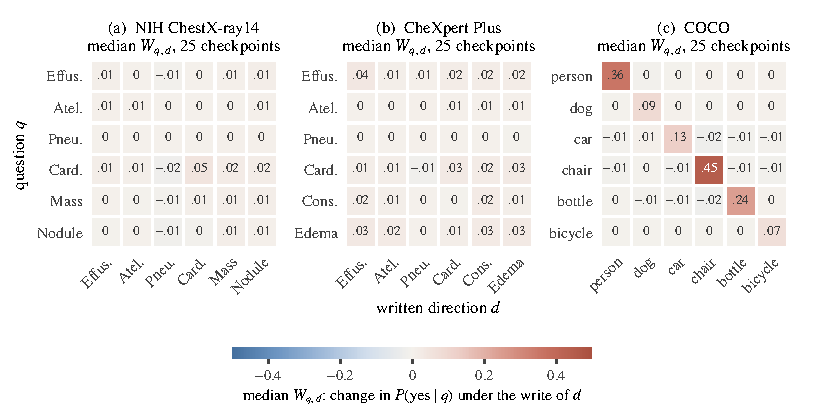
\includegraphics{figures/figA1_write_structure.pdf}}
    \caption{\textbf{Write structure across the grid.} Cell-wise median of the write matrix $W_{q,d}$ over completed checkpoints on NIH ChestX-ray14, CheXpert Plus, and COCO. Figure~\ref{fig:write-flow} reads the same matrices as flow.}
    \label{fig:cf-w-structure}
\end{figure}

\subsection{Per-image examples}
\label{app:cf-examples}

Figure~\ref{fig:cf-examples} shows grades for individual test images, with $P(\mathrm{yes})$ in parentheses on every answer line. The first four chest examples are deficit cells of Qwen2.5-VL-7B, the next two are owned cells (Lingshu 32B Edema, Qwen2.5-VL-72B Atelectasis), and the natural-image examples are owned cells of Qwen2.5-VL-7B, Lingshu 32B, and MedGemma 4B. For a chest example, we pool test rows where the finding is labelled present, the probe reads it (probability above $0.5$), and the clean answer is No. For a natural-image example, we pool rows where the probe reads the label correctly and the clean answer is No. We split each pool by whether the concept's own write or the strongest competing write raises the answer more. Among rows where either write raises the answer by at least $0.2$, we show the row with the gap closest to the median. Each example's last line reports how many pool rows share its ordering, giving the example its own base rate.

\begin{figure}[p]
    \centering
    \resizebox{\textwidth}{!}{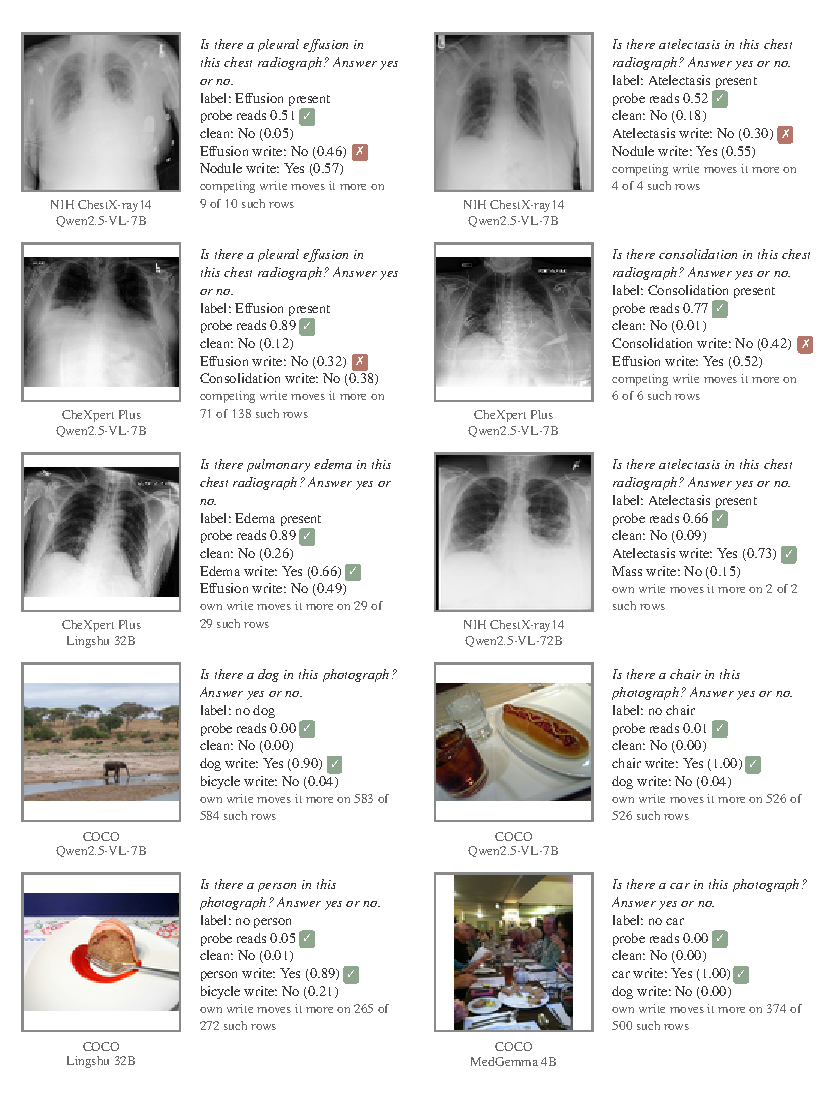
\includegraphics{figures/figA2_examples.pdf}}
    \caption{\textbf{Reading, answering, and writing on single images.} Per image: the question, the report label, the probe's reading, the clean answer, and the answers under the own write and the strongest competing write at $\alpha=+0.25$. Beside the probe's reading, a check or cross marks whether it agrees with the label; beside the own write, whether that write moves the answer more than the competitor. The grey line counts, among the block's test rows the probe reads correctly and the model answers no when clean (on the chest sets, rows labelled present), those with the same ordering.}
    \label{fig:cf-examples}
\end{figure}

\section{Pilot study: registered protocol}
\label{app:seed}

The two-model study that motivated the evaluation registered the procedures below; Appendix~\ref{app:seed-results} reports its results. It uses the construction of Section~\ref{sec:framework}, with the differences stated here.

\paragraph{Data, models, and reading.}
We use NIH ChestX-ray14 \citep{wang2017chestxray}, whose findings are mined from radiology reports. A deterministic hash of patient identity assigns rows to disjoint train, validation, and test partitions: 18,212 training images and 5,343 test images from 1,659 test patients. The three cells pair LLaVA-1.5-7B \citep{liu2024improved} with Effusion and Edema, and Qwen2.5-VL-7B \citep{bai2025qwen25vl} with Effusion, at the final visual block consumed by the connector or merger; hook tests confirm that this block lies on the downstream path, that $\alpha=0$ is a bitwise no-op, and that nonzero doses change downstream logits. Projection, scaling, and probe follow Section~\ref{sec:directions} with seed 0. Selectivity is Equation~\ref{eq:selectivity} on test rows, with 20 control seeds mapping the 39 recurring input types (AP view, sex, and age decade) to random labels and 2,000 patient-cluster bootstrap draws. Selectivity compares the concept with nuisance-type label maps of the same capacity; the write tests whether the model uses it. All uncertainty clusters by patient; prompts appear in Appendix~\ref{app:protocol}.

\paragraph{Write and doses.}
The write is Equation~\ref{eq:intervention} along the lifted normal of Equation~\ref{eq:lift}, with every entry of $\boldsymbol s$ floored at $10^{-8}$, and the endpoint is the paired mean change in $P(\mathrm{yes})$ from the common unsteered baseline (Section~\ref{sec:ownership}). Original cells use the doses $\{-1,-0.5,-0.25,-0.1,0,0.1,0.25,0.5,1\}$ on 200 held-out test images. At the six controlled doses $\mathcal A=\{\pm1,\pm0.5,\pm0.25\}$, 20 isotropic random unit directions, one coordinate-permutation sham, and the fixed alternative clinical normals receive the same signed dose on the same rows. Dose monotonicity over $[-0.5,0.5]$ is descriptive.

\paragraph{Original-cell decision rule.}
With $\Delta_c(\alpha)$ the target direction's paired mean change at dose $\alpha$, the primary effect and the dose that attains it are
\begin{equation}
\Delta^\star_c=\max_{\alpha\in\mathcal A}\operatorname{sign}(\alpha)\,\Delta_c(\alpha),\qquad
\alpha^\star=\operatorname*{arg\,max}_{\alpha\in\mathcal A}\operatorname{sign}(\alpha)\,\Delta_c(\alpha).
\label{eq:seed-rule}
\end{equation}
A cell clears the generic gate when $\Delta^\star_c$ exceeds both the 95th percentile of the 20 random directions' changes at $\alpha^\star$, each multiplied by $\operatorname{sign}(\alpha^\star)$, and the largest absolute sham effect over $\mathcal A$. The random directions are evaluated at $\alpha^\star$ alone, so the gate is a registered reference without cross-dose correction.

\paragraph{Direction-specificity supplement.}
The Nodule response motivated a separately registered supplement at the locked Qwen dose $\alpha=+0.25$, on one row per patient, chosen by label-blind hash, for 400 ChestX-ray14 test patients absent from the original cohort. It estimates the Effusion row of the write matrix (Section~\ref{sec:ownership}) against the five other pre-existing Qwen normals (Atelectasis, Pneumothorax, Cardiomegaly, Mass, and Nodule), fitted like Effusion, together with 20 random directions and the sham: 28 configurations and 11,200 per-image outcomes. Direction specificity requires an Effusion effect above the random 95th percentile and the absolute sham, and a one-sided 95\% lower bound of $O_{\mathrm{Effusion}}$ (Equation~\ref{eq:margin}) above zero, with the maximum recomputed in each of 5,000 patient-bootstrap draws. Adding competitors can only lower $O_q$, so a positive advantage holds for the family tested, while a negative one needs no exhaustive family.

\paragraph{Causal-ownership matrix.}
A prospective grid crosses six Qwen directions (Effusion, Atelectasis, Pneumothorax, Cardiomegaly, Mass, and Nodule) with their six questions on 400 new patients at $\alpha=+0.25$, with 119 random directions and a sham. Question $q$ is owned when $W_{q,q}$ exceeds every other clinical direction, every random direction, and the absolute sham, with the 30 clinical contrasts bounded simultaneously by Equation~\ref{eq:max-t}. A separate family of 12 statistics tests shared aliasing: for each direction, its signed mean effect on its five off-diagonal questions and its mean excess over the matching diagonals there.

\paragraph{Answer-encoding crossover and Mass confirmation.} A registered crossover on 200 patients of the causal-ownership cohort, with the other 200 as a patient-disjoint calibration set, crosses the original yes/no prompt with A-present and B-present prompts that exchange the finding-to-letter mapping, at $\alpha=\pm0.25$ with six clinical directions, 20 random directions, and a sham; a question enters only if both coded mappings have clean-answer AUROC lower bounds above 0.5 with at least ten patients per class. An independent confirmation then tests Mass on 200 patients absent from every earlier Qwen cohort, crossing two wordings (\textit{show}, \textit{is}) with explicit yes/no, A-present, and B-present instructions at $\alpha=+0.25$, with 119 random directions, a sham, and 20 clinical comparisons under simultaneous 95\% lower bounds. Confirmation requires positive bounds and Mass effects above every random effect and the absolute sham, across all four coded cells or both original-wording cells.


\section{Pilot study: results}
\label{app:seed-results}

\begin{table}[t]
\centering
\setlength{\tabcolsep}{4pt}
% terracotta = positive / high, blue = negative / low, sage = magnitude of Read and Ans; darker = larger magnitude
\definecolor{cfSage1}{HTML}{ECF3EF}
\definecolor{cfSage2}{HTML}{D5E5DB}
\definecolor{cfSage3}{HTML}{B9D4C3}
\definecolor{cfSage4}{HTML}{9EC3AC}
\definecolor{cfSlate1}{HTML}{EAF0F6}
\definecolor{cfSlate2}{HTML}{D0DDEA}
\definecolor{cfSlate3}{HTML}{B1C7DD}
\definecolor{cfSlate4}{HTML}{94B2D0}
\definecolor{cfTerra1}{HTML}{F7ECEA}
\definecolor{cfTerra2}{HTML}{EED5D1}
\definecolor{cfTerra3}{HTML}{E2B8B2}
\definecolor{cfTerra4}{HTML}{D79E95}
\definecolor{cfOat1}{HTML}{F4EFE6}
\definecolor{cfOat2}{HTML}{E8DDC8}
\definecolor{cfGrey}{HTML}{E4E1DC}

\caption{\textbf{Pilot replication on 600 new patients.} Qwen2.5-VL-7B on NIH ChestX-ray14. Per concept: the concept write $W_{q,q}$, the random 95th percentile (p95), the absolute sham, and its rank among the 120 compared effects; blue shades a negative ownership contrast.}
\label{tab:cf-seed}
\resizebox{\linewidth}{!}{%
\begin{tabular}{lrrrrrrrll}
\toprule
Concept & \multicolumn{1}{c}{$S$} & \multicolumn{1}{c}{AUROC} & \multicolumn{1}{c}{$W_{q,q}$} & \multicolumn{1}{c}{p95} & \multicolumn{1}{c}{$|$sham$|$} & \multicolumn{1}{c}{rank} & \multicolumn{1}{c}{$O_q$ [95\% CI]} & Competitor & Verdict\\
\midrule
Effusion & 0.102 & 0.593 & +0.190 & 0.137 & 0.017 & 2/120 & \cellcolor{cfSlate2}-0.071 [-0.080, -0.062] & Nodule & competitor \\
Atelectasis & 0.062 & 0.566 & +0.101 & 0.297 & 0.096 & 55/120 & \cellcolor{cfSlate3}-0.226 [-0.233, -0.219] & Nodule & competitor \\
Pneumothorax & 0.152 & 0.508 & +0.089 & 0.320 & 0.113 & 52/120 & \cellcolor{cfSlate3}-0.102 [-0.108, -0.096] & Effusion & competitor \\
Cardiomegaly & 0.205 & 0.742 & +0.085 & 0.311 & 0.158 & 33/120 & \cellcolor{cfSlate3}-0.219 [-0.227, -0.211] & Atelectasis & competitor \\
Mass & 0.021 & 0.678 & +0.359 & 0.372 & 0.092 & 10/120 & \cellcolor{cfSlate3}-0.169 [-0.178, -0.160] & Effusion & competitor \\
Nodule & -0.041 & 0.642 & +0.118 & 0.158 & 0.055 & 15/120 & \cellcolor{cfSlate2}-0.072 [-0.081, -0.063] & Effusion & competitor \\
\bottomrule
\end{tabular}}
\end{table}


\subsection{A non-generic write effect reproduces}
\label{sec:qwen-replication}

The first finding starts with a successful intervention: Qwen Effusion reproduces beyond random and sham controls before clinical alternatives change its attribution.

Controlled decodability is evaluated at the final visual block each connector consumes: the penultimate CLIP encoder layer for LLaVA and the last of Qwen's 32 visual blocks. Intervals are 95\% patient-cluster bootstrap intervals over 2,000 draws; the control AUROC is the mean over the 20 recurring-type random-label maps, with its 5th--95th percentile spread in parentheses.

Qwen Effusion first satisfies the reader test. Its probe reaches AUROC \cfSeedDecQwenEffAuroc{} $[\cfSeedDecQwenEffAurocLo,\cfSeedDecQwenEffAurocHi]$ against a control AUROC of \cfSeedDecQwenEffCtrl{} (\cfSeedDecQwenEffCtrlLo--\cfSeedDecQwenEffCtrlHi), a controlled selectivity of \cfSeedDecQwenEffSel{} (95\% CI $[\cfSeedDecQwenEffSelLo,\cfSeedDecQwenEffSelHi]$). LLaVA-1.5-7B reads both of its concepts at its consumed block: Effusion at AUROC \cfSeedDecLlavaEffAuroc{} $[\cfSeedDecLlavaEffAurocLo,\cfSeedDecLlavaEffAurocHi]$ with selectivity \cfSeedDecLlavaEffSel{} $[\cfSeedDecLlavaEffSelLo,\cfSeedDecLlavaEffSelHi]$, and Edema at AUROC \cfSeedDecLlavaEdemaAuroc{} $[\cfSeedDecLlavaEdemaAurocLo,\cfSeedDecLlavaEdemaAurocHi]$ with selectivity \cfSeedDecLlavaEdemaSel{} $[\cfSeedDecLlavaEdemaSelLo,\cfSeedDecLlavaEdemaSelHi]$, against a control AUROC of \cfSeedDecLlavaEffCtrl{} (\cfSeedDecLlavaEffCtrlLo--\cfSeedDecLlavaEffCtrlHi). Original-cohort intervention outcomes maximize the concept-consistent effect over six fixed nonzero doses. Qwen makes a strong write-direction case in the original 200-image cohort: the maximum concept-consistent change is 0.2343 at $\alpha=+0.25$, above the random-direction 95th percentile of 0.0963 and the maximum absolute sham effect of 0.0852.

The response at the locked dose $\alpha=+0.25$ reproduces on the patient-disjoint 400-patient cohort. Effusion changes mean $P(\mathrm{yes})$ by 0.1945, again above the random-direction 95th percentile of 0.0878 and absolute sham effect of 0.0157. None of these patients appears in the original intervention cohort, and the dose was not reselected, supporting a large and reproducible non-generic effect within ChestX-ray14.


\subsection{Semantic competition changes attribution, not efficacy}
\label{sec:specificity-results}

The fixed clinical family provides a harder identification test than non-semantic controls. Nodule changes the Effusion answer by 0.2519 and realizes the point-estimate maximum among the five alternatives. The Effusion ownership contrast $O_{\mathrm{Effusion}}$ is $-0.0573$. The registered fixed-family endpoint recomputes the maximum inside each of 5,000 patient-bootstrap draws, giving a two-sided 95\% CI of $[-0.0694,-0.0450]$ and a one-sided 95\% lower bound of $-0.0678$. The entire interval is below zero. Descriptively, all five alternative clinical normals move the Effusion endpoint in the same positive direction; Effusion exceeds four by 0.1172--0.1778, while Nodule alone has a larger point estimate. This shared-sign pattern motivates an answer-sensitive-alias hypothesis but cannot distinguish it from question-specific ownership.

Qwen Effusion therefore remains a reproducible direction that changes the answer beyond random and sham perturbations, while its specific semantic attribution fails. The familywise endpoint establishes that at least one fixed clinical alternative is stronger; Nodule is the point-estimate maximizer, not a separately familywise-identified semantic owner.

\subsection{Wording changes clinical competition for Mass}
\label{sec:encoding-results}

In the registered crossover, the four questions that pass capability calibration (Atelectasis, Pneumothorax, Mass, and Nodule) respond more in the component that reverses the raw A-minus-B sign when the finding-to-letter mapping is exchanged, but so do all 20 random directions and the sham, so aggregate mapping response does not separate clinical normals from generic perturbations. Mass is the exception: its clinical margin, the Mass effect minus the largest of the five other clinical effects in finding-present logit units, changes from $-0.7181$ under the original yes/no prompt to $0.2825$ and $0.2900$ under A-present and B-present (Table~\ref{tab:seed-mass}, top). The independent confirmation on 200 new patients reproduces the clinical advantage under both \textit{show} coded prompts, with simultaneous lower bounds of 0.1675 and 0.1462, while both \textit{is} margins are negative and the Mass effects stay below the maximum of the 119 random directions (rank 3 of 120), so neither registered specificity conjunction is met (Table~\ref{tab:seed-mass}, bottom). Mass steering increases Brier error in every cell, and every AUROC-change interval spans zero.
\begin{table}[H]
\centering
\setlength{\tabcolsep}{5pt}
\caption{\textbf{Mass clinical competition across prompts.} Clinical margin per prompt: the Mass effect minus the largest of the five other clinical effects, in finding-present logit units. Top, the discovery crossover; bottom, the registered confirmation on new patients.}
\label{tab:seed-mass}
\resizebox{\linewidth}{!}{%
\begin{tabular}{lrrrrr}
\toprule
Prompt & Clinical margin & 95\% CI & Mass effect & Random max & $|$Sham$|$ \\
\midrule
Standard yes/no & $-0.7181$ & $[-0.7956,-0.6412]$ & 2.8625 & 3.0412 & 0.5869 \\
A-present & $0.2825$ & $[0.2269,0.3406]$ & 1.6125 & 1.1650 & 0.7550 \\
B-present & $0.2900$ & $[0.2300,0.3506]$ & 1.7469 & 1.2581 & 1.1475 \\
\midrule
Condition & Clinical margin & Minimum LCB & Mass effect & Random max & \\
\midrule
\textit{show}/A-present & 0.2525 & 0.1675 & 1.7019 & 2.2100 & \\
\textit{show}/B-present & 0.2338 & 0.1462 & 1.8188 & 2.2169 & \\
\textit{is}/A-present & $-0.1087$ & $-0.1751$ & 1.9225 & 2.4750 & \\
\textit{is}/B-present & $-0.2006$ & $-0.2686$ & 2.0019 & 2.4944 & \\
\bottomrule
\end{tabular}}
\end{table}


\FloatBarrier


\section{Questions, Scores, and Notation}
\label{app:protocol}

\paragraph{Templates and score.} Each concept is asked in six templates that cross two wordings, \emph{is there} (I) and \emph{does the image show} (W), with three answer interfaces, yes/no (Y), A-present (A), and B-present (B). A template is named by its wording and its interface, and the primary template is IY. At the first answer position, $\ell_{\mathrm{yes}}$ and $\ell_{\mathrm{no}}$ are the maximum log probabilities among the valid single-token case and leading-space variants of each answer, and the registered score is $P(\mathrm{yes})=\sigma(\ell_{\mathrm{yes}}-\ell_{\mathrm{no}})$, where $\sigma$ is the logistic function. Taking the best valid variant for each answer makes the score insensitive to which capitalisation or leading-space form receives the highest probability. The score measures the relative support for yes versus no at the first answer position, not the accuracy of a generated report. Questions are the rows of $W$ and directions its columns, so changing a direction never changes the question being scored.

\paragraph{Notation.} Table~\ref{tab:notation} collects the notation of the paper.

\begin{table}[H]
\centering
\caption{Notation used in the paper.}
\label{tab:notation}
\resizebox{\linewidth}{!}{%
\begin{tabular}{l>{\raggedright\arraybackslash}p{0.867\linewidth}}
\toprule
Symbol & Definition \\
\midrule
$c$, $q$, $d$ & A concept; the yes/no question about a concept; a write direction. Questions and directions are indexed by the concept they belong to. \\
cell, block & A checkpoint--concept pair on one dataset; a checkpoint--dataset pair. \\
$\hvec_{it}$, $\hvec_i$ & Output of the consumed block for image $i$ and consumed token $t$; its mean over the consumed tokens. \\
$D$ & Hidden width of the consumed block. \\
$R$, $\boldsymbol s$, $\boldsymbol\beta_c$ & Fixed $D\times512$ Gaussian projection; training-row feature scales; logistic coefficients of concept $c$'s probe. \\
$\hat\wvec_c$ & Label direction: the probe's logit gradient $R\,\mathrm{diag}(\boldsymbol s)^{-1}\boldsymbol\beta_c$ at unit length (Equation~\ref{eq:lift}). \\
$a_q$ & Answer direction: the ridge fit of the clean answer margin $\ell_{\mathrm{yes}}-\ell_{\mathrm{no}}$, lifted in the same way. \\
$\alpha$ & Signed dose; $|\alpha|$ is the write's norm as a fraction of each token's norm. \\
$S$ & Probe selectivity: concept AUROC minus the mean AUROC of 20 random-label control probes (Equation~\ref{eq:selectivity}). \\
$W_{q,d}$ & Mean change in question $q$'s $P(\mathrm{yes})$ when direction $d$ is written. \\
$O_q$ & Ownership, $W_{q,q}-\max_{d\neq q}W_{q,d}$ (Equation~\ref{eq:margin}). \\
$O^m_q$ & Ownership computed on changes in the logit margin $\ell_{\mathrm{yes}}-\ell_{\mathrm{no}}$. \\
$\kappa_d$ & Column selectivity, $W_{d,d}/\sum_q|W_{q,d}|$. \\
$F_{q,d}$ & Mean over checkpoints of $\max(W_{q,d},0)$, the band width in Figure~\ref{fig:write-flow}. \\
$\cos_\Sigma$ & Whitened cosine under the training-feature covariance $\Sigma$ (Appendix~\ref{app:cf-ansdir}). \\
\bottomrule
\end{tabular}}
\end{table}

\FloatBarrier


\section{Joint bootstrap and simultaneous lower bounds}
\label{app:simultaneous-bounds}

For a family of $m$ statistics, let $\widehat C_j$ be statistic $j$'s estimate, $C^*_{bj}$ its value in joint bootstrap draw $b\in\{1,\dots,B\}$, and $\tau_j$ its bootstrap standard deviation with denominator $B-1$. The centred studentised draws, the common critical value, and the simultaneous lower bounds are
\begin{equation}
Z_{bj}=\frac{C^*_{bj}-\widehat C_j}{\tau_j},\qquad
c_{.95}=Q_{.95}\Bigl(\bigl\{\max_{1\leq j\leq m}Z_{bj}\bigr\}_{b=1}^{B}\Bigr),\qquad
L_j=\widehat C_j-c_{.95}\,\tau_j,
\label{eq:max-t}
\end{equation}
where $Q_{.95}$ is the empirical 95th percentile with linear interpolation. The draws are centred on the estimate, and each $\tau_j$ stays fixed across draws. A component with $\tau_j\leq10^{-12}$ gets $Z_{bj}=0$ but keeps its own $\tau_j$ in $L_j$; every draw is retained. Upper bounds use the same $c_{.95}$ with every contrast's sign reversed.

\paragraph{Verdicts.} For the ownership family of 30 contrasts $W_{q,q}-W_{q,d}$, question $q$'s simultaneous lower bound is the minimum of its five contrast bounds. The question has the advantage when that minimum is positive, a stronger competitor when any of its upper bounds is negative, and is unresolved otherwise. $O_q$ itself receives a percentile interval instead: every draw recomputes the largest competitor, the two-sided interval takes the 2.5th and 97.5th percentiles, and the pilot's Effusion supplement takes the 5th as its one-sided bound. The logit-scale grade (Appendix~\ref{app:cf-robustness}) applies both rules to margin changes.

\paragraph{Draws.} The campaign resamples the 600 test rows of each block in 2{,}000 shared draws (seed 2026090601). The pilot's ownership matrix resamples 400 patients in 5{,}000 draws (seed 20260904), with the same patient indices for every question and intervention, and bounds its shared-alias statistics as a separate family of 12. The Mass confirmation resamples 200 new patients (seed 20260910), with a family of 20 Mass-minus-alternative contrasts across four coded prompts.


\section{Reproducibility specification}
\label{app:repro}

This appendix specifies each family's consumed block, the consumed-token mask, the projection and probe, the control constructions, the cohort roles, and the protocol record at the registered protocol's level of detail. The released code implements each component.

\subsection{Consumed loci per family}
\label{app:repro-loci}

The consumed block is the last visual block that feeds the consumer. The connector locus is the consumer's output that enters the language model. We identify the block from each checkpoint's own configuration when loading the checkpoint. Each block's preflight record stores the identified block, its hidden dimension, its consumer, and any branch that bypasses it.

\begin{itemize}[leftmargin=*,itemsep=1pt,topsep=2pt]
\item Qwen2.5-VL, Lingshu, and Qwen3-VL: the merger reads the last block of the vision transformer, which has 32 blocks in Qwen2.5-VL and Lingshu, 24 in Qwen3-VL 4B, and 27 in Qwen3-VL 8B and 32B. A Qwen2.5-VL or Lingshu image contributes 576 patch tokens, which the merger joins in $2\times2$ groups into 144; a Qwen3-VL image contributes at most 1{,}024. The Qwen3-VL DeepStack mergers, which read earlier blocks, are not written.
\item Gemma~3 and MedGemma: the projector reads the last of the 27 SigLIP encoder layers through the tower's final layer normalisation, and consumes all 4{,}096 patch tokens of the $896\times896$ image.
\item InternVL3.5: the projector reads the last InternViT encoder layer, of 24 at 8B and 14B and of 45 at 38B; the tower's final normalisation is an identity in the released configuration. An image contributes 1{,}024 patch tokens from a single $448\times448$ tile.
\item LLaVA-1.5 and LLaVA-Med: the projector reads the penultimate of the 24 CLIP encoder layers, and the final layer is computed and discarded. An image contributes 576 patch tokens.
\item Llama~3.2 Vision: the projector input concatenates the last of the eight global-encoder layers with five intermediate layers of the local encoder, which bypass the consumed block. An image contributes 1{,}601 tokens, the CLS token and 1{,}600 patches, from its one real $560\times560$ tile.
\end{itemize}
Table~\ref{tab:cf-models} lists the consumed-token count of every checkpoint.

\subsection{The consumed-token mask}
\label{app:repro-mask}

The write in Equation~\ref{eq:intervention} changes only the consumed tokens at the positions the consumer reads at the locus. We derive these positions for each batch from that batch's processor outputs:

\begin{itemize}[leftmargin=*,itemsep=1pt,topsep=2pt]
\item Qwen2.5-VL, Lingshu, and Qwen3-VL: the tokens of all images in a batch form one sequence in which every image occupies one contiguous span, whose bounds follow from the image's patch grid. At the connector locus the span is a quarter as long, one merged token per $2\times2$ patch group.
\item Gemma~3 and MedGemma: all 4{,}096 patch tokens; the tower produces no CLS token. The number of written tokens must equal the number of image placeholder tokens in the language-model input.
\item InternVL3.5: the patch tokens of the single $448\times448$ tile. The CLS token, which the consumer drops, is excluded. The number of written tokens must equal the number of image placeholder tokens.
\item LLaVA-1.5 and LLaVA-Med: the 576 patch tokens. The CLS token, which the checkpoint's feature selection drops, is excluded.
\item Llama~3.2 Vision: the 1{,}601 tokens, CLS and 1{,}600 patches, of the one real $560\times560$ tile. The seven padding tokens of each tile and the three padding tiles are excluded, in agreement with the model's own aspect-ratio and cross-attention masks.
\end{itemize}

Scoring stops with an error and no fallback when an image span does not exactly cover the locus, a mask length differs from the token count at the locus, an image has no consumed token, or one forward pass reaches the locus more than once.

Preflight check (C) verifies the mask. It captures the locus tensor on a clean pass and a pass steered at $\alpha=+0.25$ along the first concept direction. It reports the maximum absolute difference outside the mask and the maximum absolute changes in the consumer's output and answer logits. Across all \cfBlocks{} blocks, the change outside the consumed tokens is $0$ at both loci. The consumer's output and answer logits both change. The same records show a bitwise-identical repeated clean pass (check A) and a bitwise-identical $\alpha=0$ pass (check B) for every block.

\subsection{Projection, lift, scaler, and probe}
\label{app:repro-probe}

We construct the projection $R\in\R^{D\times512}$ by drawing standard normal variates once from a PCG64 generator seeded with $0$, dividing by $\sqrt{512}$, and storing the result in float32. Its entries are independent $\mathcal{N}(0,1/512)$ variates. The seed is $0$ for every checkpoint, dataset, and locus. $D$ is the family's hidden dimension. We neither normalise nor orthogonalise the columns of $R$. The Gram matrix $R^{\top}R/D$ has full rank 512 in all \cfAltdirdBlocks{} blocks that carry the displacement module, with eigenvalues $\cfAltdirdEigMin$--$\cfAltdirdEigMax$ and condition number \cfAltdirdCondMin{}--\cfAltdirdCondMax{}.

Projecting the token-mean read vector $\hvec_i$ gives features $R^{\top}\hvec_i$. A featurewise standardiser fitted only on training rows supplies the mean $\boldsymbol\mu$ and scale $\boldsymbol s$. Every row is standardised as $(R^{\top}\hvec-\boldsymbol\mu)\oslash\max(\boldsymbol s,10^{-8})$, where $\oslash$ and $\max$ act elementwise. Each concept probe is an $\ell_2$-regularised logistic regression with inverse regularisation strength $C=1$. We fit each probe by L-BFGS for at most 2{,}000 iterations with unweighted classes and seed $0$, using training rows with a known label for that concept. For each of the two refit seeds, we resample training units with replacement, retaining all rows of each sampled unit at its multiplicity. We then refit the scaler and six probes using the same projection. The random family, shams, and control probes remain at seed 0.

\subsection{Control constructions}
\label{app:repro-controls}

\paragraph{Random directions.} We draw one $119\times D$ standard-normal matrix using a PCG64 generator seeded with $0$ and normalise each row to unit $\ell_2$ norm. Every question in the block uses the same 119 directions.

\paragraph{Coordinate-permutation sham.} Immediately after the random draw, the same generator produces one permutation of $\{0,\dots,D{-}1\}$ per concept, in protocol concept order. We form concept $c$'s sham by rearranging the coordinates of $\hat\wvec_c$ with concept $c$'s own permutation. This preserves the direction's coordinate multiset and unit norm. We write each question with its own sham.

\paragraph{Matched random-label probes.} Each row has a type: view $\times$ sex $\times$ age decade on the chest sets, and aspect-ratio $\times$ area buckets on COCO. For control seed $k\in\{0,\dots,19\}$, we traverse the types in sorted order and use a PCG64 generator seeded with $k$ to draw one label per type uniformly from $\{0,1\}$. If all types receive the same label, we flip the first. Every row of a type receives that type's label. We give each control probe the concept probe's capacity and nuisance structure by fitting it on the same training rows and known-label subset with the same hyperparameters. A block fits control probes when its training rows span at least eight types. Selectivity is Equation~\ref{eq:selectivity}. Its bootstrap over calibration units retains a draw when the real AUROC is finite and at least ten of the twenty control AUROCs are finite. We grade a cell for readability when at least 1{,}900 of the 2{,}000 draws are retained.

\subsection{Cohort roles}
\label{app:repro-cohorts}

Every chest image is a frontal study. One role holds more than one row per unit: the NIH training role, which takes every study of each training patient, \cfCohortNihTrainRows{} studies from \cfCohortNihTrainUnits{} patients, \cfCohortNihTrainMulti{} of whom contribute more than one and one of whom contributes \cfCohortNihTrainMax{}. Every other role of every dataset holds one row per unit, and no unit appears in two roles of a dataset. We use the calibration role only to determine readability and answerability. We neither fit probes nor score writes on it. Every write uses the test role.

\FloatBarrier

\subsection{Protocol amendments}
\label{app:repro-protocol}

Every analysis the paper reports beyond the \cfCoveragePlannedWord{} planned modules was added to the protocol file as a dated amendment after the first wave, and each amendment precedes the first result of the module it registers. Each amendment entry names its own rows, references, and decision rule before it names a result.


\FloatBarrier

\paragraph{The fine-grained category selection rule.} The rule that picks the six fine-grained COCO categories is stated in the protocol file in full, and it reads on the labels alone. A category is eligible when its training positives are at least as many as the weakest of the six existing concepts, when it has at least ten positives among the 400 calibration rows and at least ten among the 600 test rows, and when its mean relative instance area is below the median of the six existing concepts. Eligible categories are ranked by calibration positives in descending order, ties by mean relative instance area in ascending order, and remaining ties by category identifier; the first six are taken. The rule uses the label counts and the instance areas of the fixed cohorts and nothing else: no probe, no answer, and no write enters it. The protocol file carries the rule under the date of its amendment, and the module's first result is later than that date, so the six categories and the two matching windows were fixed before any of them was scored.

\end{document}
